%%%%%%%%%%%%%%%%%%%%%%%%%%%%%%%%%%%%%%%%%%%%%%%%%%%%%%%%%%%%%%%
%% BRIEF VERSION OF OXFORD THESIS TEMPLATE FOR CHAPTER PREVIEWS

%%%%% CHOOSE PAGE LAYOUT
% format for PDF output (ie equal margins, no extra blank pages):
\documentclass[a4paper,nobind]{templates/ociamthesis}

% UL 5 January 2021 - add packages used by kableExtra
\usepackage{booktabs}
\usepackage{longtable}
\usepackage{array}
\usepackage{multirow}
\usepackage{wrapfig}
\usepackage{colortbl}
\usepackage{pdflscape}
\usepackage{tabu}
\usepackage{threeparttable}
\usepackage{threeparttablex}
\usepackage[normalem]{ulem}
\usepackage{makecell}
\usepackage[colorlinks=false,pdfpagelabels,hidelinks=]{hyperref}
\usepackage{float}


%UL set section header spacing
\usepackage{titlesec}
% 
\titlespacing\subsubsection{0pt}{24pt plus 4pt minus 2pt}{0pt plus 2pt minus 2pt}

% UL 30 Nov 2018 pandoc puts lists in 'tightlist' command when no space between bullet points in Rmd file
\providecommand{\tightlist}{%
  \setlength{\itemsep}{0pt}\setlength{\parskip}{0pt}}
 
% UL 1 Dec 2018, fix to include code in shaded environments
\usepackage{color}
\usepackage{fancyvrb}
\newcommand{\VerbBar}{|}
\newcommand{\VERB}{\Verb[commandchars=\\\{\}]}
\DefineVerbatimEnvironment{Highlighting}{Verbatim}{commandchars=\\\{\}}
% Add ',fontsize=\small' for more characters per line
\usepackage{framed}
\definecolor{shadecolor}{RGB}{248,248,248}
\newenvironment{Shaded}{\begin{snugshade}}{\end{snugshade}}
\newcommand{\AlertTok}[1]{\textcolor[rgb]{0.94,0.16,0.16}{#1}}
\newcommand{\AnnotationTok}[1]{\textcolor[rgb]{0.56,0.35,0.01}{\textbf{\textit{#1}}}}
\newcommand{\AttributeTok}[1]{\textcolor[rgb]{0.77,0.63,0.00}{#1}}
\newcommand{\BaseNTok}[1]{\textcolor[rgb]{0.00,0.00,0.81}{#1}}
\newcommand{\BuiltInTok}[1]{#1}
\newcommand{\CharTok}[1]{\textcolor[rgb]{0.31,0.60,0.02}{#1}}
\newcommand{\CommentTok}[1]{\textcolor[rgb]{0.56,0.35,0.01}{\textit{#1}}}
\newcommand{\CommentVarTok}[1]{\textcolor[rgb]{0.56,0.35,0.01}{\textbf{\textit{#1}}}}
\newcommand{\ConstantTok}[1]{\textcolor[rgb]{0.00,0.00,0.00}{#1}}
\newcommand{\ControlFlowTok}[1]{\textcolor[rgb]{0.13,0.29,0.53}{\textbf{#1}}}
\newcommand{\DataTypeTok}[1]{\textcolor[rgb]{0.13,0.29,0.53}{#1}}
\newcommand{\DecValTok}[1]{\textcolor[rgb]{0.00,0.00,0.81}{#1}}
\newcommand{\DocumentationTok}[1]{\textcolor[rgb]{0.56,0.35,0.01}{\textbf{\textit{#1}}}}
\newcommand{\ErrorTok}[1]{\textcolor[rgb]{0.64,0.00,0.00}{\textbf{#1}}}
\newcommand{\ExtensionTok}[1]{#1}
\newcommand{\FloatTok}[1]{\textcolor[rgb]{0.00,0.00,0.81}{#1}}
\newcommand{\FunctionTok}[1]{\textcolor[rgb]{0.00,0.00,0.00}{#1}}
\newcommand{\ImportTok}[1]{#1}
\newcommand{\InformationTok}[1]{\textcolor[rgb]{0.56,0.35,0.01}{\textbf{\textit{#1}}}}
\newcommand{\KeywordTok}[1]{\textcolor[rgb]{0.13,0.29,0.53}{\textbf{#1}}}
\newcommand{\NormalTok}[1]{#1}
\newcommand{\OperatorTok}[1]{\textcolor[rgb]{0.81,0.36,0.00}{\textbf{#1}}}
\newcommand{\OtherTok}[1]{\textcolor[rgb]{0.56,0.35,0.01}{#1}}
\newcommand{\PreprocessorTok}[1]{\textcolor[rgb]{0.56,0.35,0.01}{\textit{#1}}}
\newcommand{\RegionMarkerTok}[1]{#1}
\newcommand{\SpecialCharTok}[1]{\textcolor[rgb]{0.00,0.00,0.00}{#1}}
\newcommand{\SpecialStringTok}[1]{\textcolor[rgb]{0.31,0.60,0.02}{#1}}
\newcommand{\StringTok}[1]{\textcolor[rgb]{0.31,0.60,0.02}{#1}}
\newcommand{\VariableTok}[1]{\textcolor[rgb]{0.00,0.00,0.00}{#1}}
\newcommand{\VerbatimStringTok}[1]{\textcolor[rgb]{0.31,0.60,0.02}{#1}}
\newcommand{\WarningTok}[1]{\textcolor[rgb]{0.56,0.35,0.01}{\textbf{\textit{#1}}}}

%UL 2 Dec 2018 add a bit of white space before and after code blocks
\renewenvironment{Shaded}
{
  \vspace{10pt}%
  \begin{snugshade}%
}{%
  \end{snugshade}%
  \vspace{8pt}%
}
%UL 2 Dec 2018 reduce whitespace around verbatim environments
\usepackage{etoolbox}
\makeatletter
\preto{\@verbatim}{\topsep=0pt \partopsep=0pt }
\makeatother

%UL 28 Mar 2019, enable strikethrough
\usepackage[normalem]{ulem}

%UL use soul package for correction highlighting
\usepackage{soul}
\usepackage{xcolor}
\newcommand{\ctext}[3][RGB]{%
  \begingroup
  \definecolor{hlcolor}{#1}{#2}\sethlcolor{hlcolor}%
  \hl{#3}%
  \endgroup
}
\soulregister\ref7
\soulregister\cite7
\soulregister\autocite7
\soulregister\textcite7
\soulregister\pageref7

%UL 3 Nov 2019, avoid mysterious error from not having hyperref included
\usepackage{hyperref}

%%%%% SELECT YOUR DRAFT OPTIONS
% Three options going on here; use in any combination.  But remember to turn the first two off before
% generating a PDF to send to the printer!

% This adds a "DRAFT" footer to every normal page.  (The first page of each chapter is not a "normal" page.)

% This highlights (in blue) corrections marked with (for words) \mccorrect{blah} or (for whole
% paragraphs) \begin{mccorrection} . . . \end{mccorrection}.  This can be useful for sending a PDF of
% your corrected thesis to your examiners for review.  Turn it off, and the blue disappears.

%%%%% BIBLIOGRAPHY SETUP
% Note that your bibliography will require some tweaking depending on your department, preferred format, etc.
% The options included below are just very basic "sciencey" and "humanitiesey" options to get started.
% If you've not used LaTeX before, I recommend reading a little about biblatex/biber and getting started with it.
% If you're already a LaTeX pro and are used to natbib or something, modify as necessary.
% Either way, you'll have to choose and configure an appropriate bibliography format...

% The science-type option: numerical in-text citation with references in order of appearance.
% \usepackage[style=numeric-comp, sorting=none, backend=biber, doi=false, isbn=false]{biblatex}
% \newcommand*{\bibtitle}{References}

% The humanities-type option: author-year in-text citation with an alphabetical works cited.
% \usepackage[style=authoryear, sorting=nyt, backend=biber, maxcitenames=2, useprefix, doi=false, isbn=false]{biblatex}
% \newcommand*{\bibtitle}{Works Cited}

%UL 3 Dec 2018: set this from YAML in index.Rmd
\usepackage[style=authoryear, sorting=nyt, backend=biber, maxcitenames=2, useprefix, doi=false, isbn=false]{biblatex}
\newcommand*{\bibtitle}{Works Cited}

% This makes the bibliography left-aligned (not 'justified') and slightly smaller font.
\renewcommand*{\bibfont}{\raggedright\small}

% Change this to the name of your .bib file (usually exported from a citation manager like Zotero or EndNote).
\addbibresource{references.bib}

%%%%% YOUR OWN PERSONAL MACROS
% This is a good place to dump your own LaTeX macros as they come up.

% To make text superscripts shortcuts
	\renewcommand{\th}{\textsuperscript{th}} % ex: I won 4\th place
	\newcommand{\nd}{\textsuperscript{nd}}
	\renewcommand{\st}{\textsuperscript{st}}
	\newcommand{\rd}{\textsuperscript{rd}}

%%%%% THE ACTUAL DOCUMENT STARTS HERE
\begin{document}

%%%%% CHOOSE YOUR LINE SPACING HERE
% This is the official option.  Use it for your submission copy and library copy:
\setlength{\textbaselineskip}{22pt plus2pt}
% This is closer spacing (about 1.5-spaced) that you might prefer for your personal copies:
%\setlength{\textbaselineskip}{18pt plus2pt minus1pt}

% UL: You can set the general paragraph spacing here - I've set it to 2pt (was 0) so
% it's less claustrophobic
\setlength{\parskip}{2pt plus 1pt}

% Leave this line alone; it gets things started for the real document.
\setlength{\baselineskip}{\textbaselineskip}

% all your chapters and appendices will appear here
\hypertarget{transformation-of-microfinance-institutions-and-its-effects-on-financial-inclusion-in-africa-mfi-transformation-and-financial-inclusion}{%
\section{Transformation of Microfinance Institutions and its Effects on Financial Inclusion in Africa \{\#MFI Transformation and Financial Inclusion\}}\label{transformation-of-microfinance-institutions-and-its-effects-on-financial-inclusion-in-africa-mfi-transformation-and-financial-inclusion}}

\minitoc 

\hypertarget{abstract}{%
\section{\texorpdfstring{\textbf{Abstract}}{Abstract}}\label{abstract}}

\begin{quote}
The shift away from the not-for-profit microfinance institutions (MFIs) model has seen the rise of commercial MFIs in forms like commercial banks, credit unions, and rural banks and the not-for-profit, non-governmental organisations (NGOs). The shift arose partly due to neo-liberalism and the need for MFIs to reach the financially excluded more sustainably than had been the case. Therefore, this article examines how the shift has affected financial inclusion in Africa, utilising data from the Microfinance Information Exchange (MIX). Our results show that the change from the NGO model to the commercial models could negatively affect the depth of financial outreach, especially given that NGOs characteristically have better outreach to women and advance smaller denomination loans on average. Also, NGOs have higher median gross loans than other legal forms of MFIs except for credit unions/ cooperatives, although commercial banks have the highest average gross loans. These results remain robust upon removing outliers and controlling for factors that affect the ability of MFIs to offer financial services to the poor.
\end{quote}

\newpage

\hypertarget{background}{%
\section{\texorpdfstring{\textbf{Background}}{Background}}\label{background}}

In 1992, PRODEM, a micro-finance institution (MFI) in Bolivia, converted from a non-governmental organisation (NGO) to a commercial bank, BANCOSOL. In fact, in the immediate past three decades, numerous NGO MFIs across the globe have adopted the commercial forms of microfinance (Table 1). In this article, we examine how the conversion of MFIs to the commercial model affects financial inclusion in terms of the depth and breadth of outreach to the financially excluded. Depth refers to the extent of the traditional financially excluded clients reached by MFIs. If an MFI serves more financially excluded people like women and the poor, it has deeper outreach.

On the other hand, breadth refers to the sheer number of clients reached regardless of their level of financial exclusion. Thus, an MFI that offers more loans to many people has more breadth of outreach. In other words, we explore how the transformation of MFIs typically drives their average loan balance per borrower, the proportion of women borrowers and gross loans. The former two metrics capture depth while the latter proxies breadth.

The study focuses on Africa, a continent that is the epicentre of financial exclusion despite remarkable economic progress of the last three decades \autocite{beck2014sme,allen2011african}. Evaluating the effects of transformation by using global metrics is likely to mask regional heterogeneity, given that these effects could manifest differently in varying settings \autocite{d2017ngos,d2013unsubsidized} \footnote{We use the terms financial sustainability/ efficiency/ profitability on the one hand and social performance/ outreach on the other interchangeably. By Financial sustainability, we refer to the capability of a firm to turn a profit, which allows it to meet its obligations without relying on donations and subsidies. Social performance/ outreach is the firm's ability to reach out and avail financial services to the financially excluded members of society, including the poor, women, and rural dwellers- referring to both breadth and depth.}.

Most pioneer microfinance institutions adopted a not-for-profit model \autocite{dichter1996questioning}, operating mainly as non-governmental organisations (NGOs). However, the dominance of neo-liberalism in organising production has seen many donors scale back and push MFIs to strive for financial sustainability \autocite{bateman2010doesn}. The arguments for the commercial approach to running microfinance activities revolve around sustainability. The financial sustainability school posits that MFIs can best serve the financially excluded when they have a degree of financial self-sufficiency \autocite{kodongo2013individual}. For instance, profit-oriented MFIs could offer financial services to the relatively well-off at market rates and use the proceeds (profits) to subsidise services to the poor more than relying on donations and subsidies alone. Hence, MFIs pursuing the for-profit model may experience mission expansion \autocite{mersland2010microfinance,louis2013financial}. Also, donor funds are volatile and subject to political and economic conditions \autocite{garmaise2013cheap,d2017aid}. In this respect, a substantial body of research finds that the transformation of microfinance institutions enhances outreach to the financially excluded \autocite{frank2008stemming,gutierrez2009social,mersland2010microfinance,quayes2012depth,mia2017mission,d2013unsubsidized}.

The proponents of MFI transformation point to the concerning possibility of mission drift. Mission drift happens when MFIs focus less on providing financial services to the financially excluded in favour of making profits. Some researchers have found this to be the case \autocite{louis2013financial,bos2015practice,d2013unsubsidized,hartarska2012governance}. Two theories can be said to underpin the MFI transformation phenomenon. The first is the agency theory on the conflicts between providers of capital and managers. In a quest to minimise agency conflicts, managers may consciously or sub-consciously place less emphasis on the social mission of MFIs, reaching out to the financially excluded. Instead, managers may more overtly focus on pursuing financial returns for shareholders and debt-holders, thus causing mission drift. The theory presumes that the motivation for all fund providers is financial returns, which is not always the case.

The second one, the institutional theory, examines the rise, persistence and decline of institutional structures over time. The central question here is; What drives the adoption and fall of certain institutional norms \autocite{powell2012new}? In this respect, some institutionalists claim that prevailing institutional culture is more potent than market forces in driving the adoption or rejection of emergent institutional structures. Institutionalists posit that one of the drivers is coercion. In the case of MFIs, some donors have put implicit or explicit pressure on financial sustainability.

Additionally, the adoption of institutional norms in most cases arises out of the need to fit into the institutional environment. The desire to be compliant may explain the prevalence of NGOs not-for-profit type MFIs in the early years of the microfinance paradigm and the trend towards the transformation of MFIs to commercial entities that is now ongoing. Notably, institutional theory sheds light on the dilemmas managers face when institutional norms change \autocite{thornton2015institutional}. For instance, how can managers of MFIs reconcile financial sustainability with the original priority of outreach to the financially excluded?

\begin{Shaded}
\begin{Highlighting}[]
\FunctionTok{library}\NormalTok{(tibble)}

\FunctionTok{tribble}\NormalTok{(}\SpecialCharTok{\textasciitilde{}}\NormalTok{ Institution, }\SpecialCharTok{\textasciitilde{}}\NormalTok{ Country, }\SpecialCharTok{\textasciitilde{}}\NormalTok{ Year, }\SpecialCharTok{\textasciitilde{}}\NormalTok{ Converted\_to,}
        \StringTok{"Finansol"}\NormalTok{, }\StringTok{"Colombia"}\NormalTok{, }\StringTok{"1993"}\NormalTok{, }\StringTok{"Commercial Finance Company"}\NormalTok{,}
        \StringTok{"OIBM"}\NormalTok{, }\StringTok{"Malawi"}\NormalTok{, }\StringTok{"2002"}\NormalTok{, }\StringTok{"NBFI"}\NormalTok{,}
        \StringTok{"PRIDE"}\NormalTok{, }\StringTok{"Tanzania"}\NormalTok{, }\StringTok{"2009"}\NormalTok{, }\StringTok{"NBFI"}\NormalTok{,}
        \StringTok{"Kenya Women Finance Trust"}\NormalTok{, }\StringTok{"Kenya"}\NormalTok{, }\StringTok{"2010"}\NormalTok{, }\StringTok{"NBFI"}\NormalTok{,}
        \StringTok{"Faulu"}\NormalTok{, }\StringTok{"Kenya"}\NormalTok{, }\StringTok{"2010"}\NormalTok{, }\StringTok{"NBFI"}\NormalTok{,}
        \StringTok{"OI{-}SASL"}\NormalTok{, }\StringTok{"Ghana"}\NormalTok{, }\StringTok{"2013"}\NormalTok{, }\StringTok{"NBFI"}\NormalTok{) }\SpecialCharTok{\%\textgreater{}\%}
  
  \FunctionTok{kbl}\NormalTok{(., }\AttributeTok{caption =} \StringTok{"Sample of Transformed MFIs"}\NormalTok{, }
      
      \AttributeTok{booktabs =} \ConstantTok{TRUE}\NormalTok{) }\SpecialCharTok{\%\textgreater{}\%} 
  
  \FunctionTok{kable\_paper}\NormalTok{(}\AttributeTok{full\_width =} \ConstantTok{FALSE}\NormalTok{, }\AttributeTok{font\_size =} \DecValTok{10}\NormalTok{) }\SpecialCharTok{\%\textgreater{}\%} 
  
  \FunctionTok{footnote}\NormalTok{(}\AttributeTok{general =} \StringTok{"Source: Authors\textquotesingle{} construction from the literature"}\NormalTok{,}
           
           \AttributeTok{general\_title =} \StringTok{""}\NormalTok{,}
           
           \AttributeTok{number =} \FunctionTok{c}\NormalTok{(}\StringTok{"This is a snapshot of the many MFIs that have converted over the years accross the globe"}\NormalTok{),}
           \AttributeTok{number\_title =} \StringTok{"Note: "}\NormalTok{)}
\end{Highlighting}
\end{Shaded}

\begin{table}

\caption{\label{tab:unnamed-chunk-2}Sample of Transformed MFIs}
\centering
\fontsize{10}{12}\selectfont
\begin{tabular}[t]{llll}
\toprule
Institution & Country & Year & Converted\_to\\
\midrule
Finansol & Colombia & 1993 & Commercial Finance Company\\
OIBM & Malawi & 2002 & NBFI\\
PRIDE & Tanzania & 2009 & NBFI\\
Kenya Women Finance Trust & Kenya & 2010 & NBFI\\
Faulu & Kenya & 2010 & NBFI\\
\addlinespace
OI-SASL & Ghana & 2013 & NBFI\\
\bottomrule
\multicolumn{4}{l}{\rule{0pt}{1em}Source: Authors' construction from the literature}\\
\multicolumn{4}{l}{\rule{0pt}{1em}\textit{Note: }}\\
\multicolumn{4}{l}{\rule{0pt}{1em}\textsuperscript{1} This is a snapshot of the many MFIs that have converted over the years accross the globe}\\
\end{tabular}
\end{table}

As noted earlier, research outcomes on the effects of the transformation of microfinance institutions are mixed. \textcite{morduch2019challenges} argue that if commercial MFIs could sustainably achieve financial sustainability while also reaching the poor, NGOs would not exist. In that context, therefore, the most critical question relates to how the transformation of MFIs would affect their core mission of providing financial services to the financially excluded. The issue is vital due to the legitimacy that MFIs derive from serving the financially excluded. Besides, financial inclusion is central to alleviating poverty and achieving inclusive growth, an essential dimension of financial development. In this article, we use data from the Microfinance Information Exchange (MIX) to evaluate the ways that the transformation of MFIs affects financial inclusion in Africa.

We capture the extent of financial inclusion in Africa by using three metrics:

\begin{itemize}
\tightlist
\item
  The percentage of female borrowers.
\item
  Average loan balance per borrower.
\item
  The ratio of the gross loan portfolio to total assets of each MFI \autocite{d2017ngos}.
\end{itemize}

The first two metrics proxy the depth of outreach, with more significant outreach to women indicating deeper outreach, given that women form a substantial proportion of the financially excluded population in Africa \autocite{ayyagari2013financing}. A higher average loan balance per borrower, on the other hand, corresponds to a lower depth of outreach to any group of the financially excluded. The presumption is that financially excluded people usually borrow in smaller denominations that have drawn reservations from some researchers who argue poor people could progressively demand bigger loans as they get better off. Also, MFIs regularly use progressive lending where people who successfully pay off loans qualify for larger loan amounts. Finally, gross loans to assets capture the breadth of outreach, with higher ratios indicating more breadth.

We have organised the rest of the article as follows. Section 1.1 highlights the results of the study. In section 2, we review the background literature on MFI transformation. In section 3, we describe the methodology and, in section 4, we present and discuss the results and close with concluding remarks in section 5.

\hypertarget{summary-of-results}{%
\subsection{\texorpdfstring{\textbf{Summary of Results}}{Summary of Results}}\label{summary-of-results}}

Overall, we find that the conversion away from the NGO, not-for-profit model in Africa is harmful to financial inclusion's depth and breadth. NGO-type MFIs consistently outperform the commercial-oriented MFIs regarding the outreach to women borrowers. Additionally, NGO-type MFIs have the lowest average loan balance per borrower, indicating that they reach out to the poorest and, presumably, more financially excluded people. Turning to the ratio of gross loans to assets, NGO-type MFIs come second to credit unions/ cooperatives, thus indicating that breadth and depth of outreach are not necessarily mutually exclusive. Further examination of the trend suggests that profit-oriented MFIs reflect a measure of mission drift.

On the one hand, serving poor, financially excluded people is costly, which hurts the profitability of MFIs. On the other hand, profit orientation implies commercial capital, interest expense on debt capital and dividends on equity capital. If it is hard to reconcile these two objectives, we are inclined to back the literature that opposes the commercialisation of MFIs. As we shall see later, it seems odd that NGO-type MFIs lend more gross loans (breadth) than most commercial-oriented MFIs, though it turns out that both cooperatives and NGO-type MFIs hold the lowest volume of assets relative to other legal types. Furthermore, the other important drivers of financial inclusion are the age of MFI, operating expense to assets ratio, donations to assets ratio, capital to assets ratio, asset structure, size, education and profit margin. In the next section, we highlight the methodology and then go to the details of the results.

\hypertarget{theory-and-empirical-literature}{%
\section{\texorpdfstring{\textbf{Theory and Empirical Literature}}{Theory and Empirical Literature}}\label{theory-and-empirical-literature}}

The extent to which the transformation of MFIs affects financial inclusion has been the subject of substantial research. However, there is a lack of consensus on the outcomes about its effects. Theories underlying aspects of the transformation of MFIs are the agency theory \autocite{jensen1976theory} and institutional theory \autocite{powell2012new}. Agency theory, in this case, implies that injection of commercial capital, a consequence of transformation, is likely to motivate managers to target financial return at the expense of social return to satisfy shareholders and debt-holders, the conventional providers of commercial capital. From this perspective, transformation implies that mission drift is inevitable. Indeed, \textcite{morduch2019challenges} argue that if mission drift is not an issue in microfinance, then the NGOs MFI model would not exist, meaning that NGOs (not-for-profit) MFIs exist to fill a gap left by commercial MFIs.

The institutionalists weigh how specific organisational structures dominate and ultimately decline and get discarded \autocite{powell2012new}. Institutionalists note that in certain situations, people adopt given structures without critical scrutiny to fit into the prevailing institutional environment merely. This argument could partly explain the prevalence of NGO MFI models at the early stages of microfinance evolution and the current rise of MFI commercialisation. However, the pressure to change takes several forms, with the most notable one being coercive pressure, where stakeholders put forth overt or covert pressure for MFIs to convert. In the case of MFIs, the pressure to adopt a commercial model came with the rise of neo-liberal thought around production and its funding \autocite{bateman2010doesn}, with major donors like USAID signalling their expectation that MFIs should become more financially sustainable going forward \autocite{d2013unsubsidized}. The problem for MFIs that transform is how best to balance between social goals of reaching the poor and the commercial goals that come with commercial capital and the attendant decline of donor funding.

\textcite{thornton2002rise} and \textcite{thornton2015institutional} note that ``the meaning and legitimacy of various sources of organisational identity, strategy and structure are shaped by a prevailing institutional logic''. The management of transformed MFIs can identify with microfinance as a social pursuit by emphasising social goals over profits. Alternatively, they may view microfinance as a financial venture by placing profits over social outreach. The former corresponds to the welfare model of microfinance, which posits that the social mission of microfinance is incompatible with the profit motive. The latter is the financial sustainability model, which views financial returns as a precondition for the sustainable pursuit of financial services goals of reaching the financially excluded. A third model, the win-win approach, attempts to reconcile the welfare and sustainability approach by proposing that financial and social performance are not always substituting but complementary. Different researchers have availed evidence in support of either school, as described next.

As noted, support for MFI transformation rests on two primary grounds. First, donations are subject to social, economic, and political conditions \autocite{garmaise2013cheap,armendariz2013subsidy,d2017aid}. Consequently, some researchers argue that microfinance can only be sustainable if MFIs have a level of financial self-sufficiency. In this regard, these scholars note that MFIs could advance financial services to the financially well-off and use the proceeds (profits) to reach more financially excluded people at subsidised rates, which would then lead to ``mission expansion'' as opposed to ``mission drift''. \textcite{frank2008stemming} provides empirical support for these arguments noting that transformed MFIs score higher in terms of client outreach and the number of female clients reached, although the proportion of female clients reached declines. They also find that transformed MFIs record higher growth in gross loan portfolio with better product diversification.

Similarly, \textcite{d2017ngos} finds that transformed MFIs charge a lower interest rate to micro-borrowers. \textcite{louis2013financial}, using self-organising maps and k-means clustering, find a positive relationship between financial sustainability and social performance to imply that steps to enhance financial sustainability are good. Other researchers that have found a positive link between financial and social efficiency include \textcite{gutierrez2009social}, \textcite{mersland2010microfinance}, and \textcite{quayes2012depth}.

In contrast to the above findings, several researchers have found transformation to be harmful in terms of outreach to the financially excluded. For instance, \textcite{d2017ngos} find that although transformed MFIs charge lower interest and experience a drop in operating expenses, their average loan sizes increase, indicative of mission drift. \textcite{mia2017mission} also find a trade-off between depth of outreach and the profit motive of MFIs in Bangladesh using both static and dynamic panel data methods. \textcite{d2013unsubsidized} notes that MFIs with little or no subsidies exhibit more significant mission drift. In our case, NGOs have the highest donations, implying that they may show greater social inclination. For instance, firms in Africa and Asia compensate for low subsidies by charging higher interest rates, while Latin America serves fewer women. In Europe and Central Asia, the tendency is to serve fewer indigent clients. \textcite{bos2015practice} also notes that MFIs that stay close to their original mission are the most socially efficient, while those that attempt to pursue a double bottom line are relatively inefficient. Further, they note that not all MFIs suffer mission drift the same way, arguing that MFIs with high input-output efficiency may not experience mission drift at all.

Besides, \textcite{campion1999institutional} argue that the presence or absence of mission drift in a transformed MFI is a corporate governance issue and an outcome of the challenges of the scaling up of MF services. They argue that good corporate governance allows the management to balance between financial performance and outreach. It means that MFIs could address mission drift problems through proper corporate governance regardless of whether an MFI is an NGO or commercial-type entity. Moreover, \textcite{marti2016financial} argue that different social groups such as employees, management, and MFI clients are likely to have different views, including varying definitions of social welfare. Thus, the presence or absence of mission drift may not arise from deliberate management decisions but instead from conflicting viewpoints on the meaning of social welfare between stakeholders. Given the conflicting evidence and varying views regarding mission drift in MFIs, the arguments by \textcite{morduch1999microfinance} and \textcite{morduch2000microfinance} that the microfinance industry should accommodate different legal forms of MFIs to serve different clients' needs appear to be valid.

\hypertarget{method}{%
\section{\texorpdfstring{\textbf{Method}}{Method}}\label{method}}

We run fixed and random effects models based on the results of the Hausmann Tests (see Appendix 1). The design of fixed effects models allows for the study of the causes of changes within an entity. It accomplishes this by controlling for all time-invariant differences between the individuals, so the estimated coefficients of the fixed-effects models cannot be biased because of omitted time-invariant characteristics, such as culture \autocite{torres2007panel}. On the other hand, Random effect models assist in controlling for unobserved heterogeneity when the heterogeneity is constant over time and uncorrelated with the explanatory variables. Following \textcite{roberts2013endogeneity}, we fit the following model.

\begin{equation}
y_{it} = \hat{a} + \hat{b}x_{it} + \mu_{it}
\end{equation}

In this case, \(y_{it}\) is the independent variable; interchangeably represented by per cent of female borrowers, average loan balance per borrower, and gross loan portfolio to total assets. The first two metrics capture financial depth, while gross loans capture the breadth of outreach.

Also, \(x_{it}\) is a matrix of independent variables. The variable of interest in our case is the current legal form of the MFI, which enters the model as a dummy representing NGOs, NBFIs, commercial banks, rural banks and credit unions/ cooperatives \autocite{ayyagari2013financing}. The other control variables include age dummy, a dummy for region, operating expenses to assets ratio, donations to assets ratio, equity capital to assets ratio, asset structure, size (logarithm of total assets), education, and profit margin all of which are derived from the literature \autocite{ayyagari2013financing,d2017ngos,d2013unsubsidized}.

Finally, \(\mu_{it}\) is the error term that we assume has zero mean conditional on \(x_{it}\).

Further,

\begin{equation}
\mu_{it} = c_{i} + \varepsilon_{it}
\end{equation}

In the equation, \(c_{i}\) captures the aggregate effects of the unobserved, time-invariant explanatory variables for \(y_{it}\).

In the case where \(c_{i}\) and \(x_{it}\) are correlated, then \(c_{i}\) is a fixed effect, otherwise, it is a random effect. Note that the existence of fixed effects implies the presence of endogeneity. For random effects, on the other hand, endogeneity is not a concern. However, the random-effects model affects the computation of standard errors \autocite{roberts2013endogeneity}. To eliminate the fixed effect prone to endogeneity, we run the within estimator model \autocite{clark2015should}. We present the results from the estimation of the empirical model in the next section.

\hypertarget{results}{%
\section{\texorpdfstring{\textbf{Results}}{Results}}\label{results}}

In this section, we begin by visualizing the study variables followed by summary statistics of the variables. We then run and discuss the results of the regression model.

\begin{Shaded}
\begin{Highlighting}[]
\DocumentationTok{\#\# legal traditions }
\DocumentationTok{\#\#\# Common law countries in Africa}
\NormalTok{common }\OtherTok{\textless{}{-}} \FunctionTok{tibble}\NormalTok{(}\AttributeTok{country =} \FunctionTok{c}\NormalTok{(}\StringTok{"Botswana"}\NormalTok{, }\StringTok{"Gambia, The"}\NormalTok{, }\StringTok{"Ghana"}\NormalTok{, }\StringTok{"Kenya"}\NormalTok{, }\StringTok{"Lesotho"}\NormalTok{, }\StringTok{"Liberia"}\NormalTok{, }\StringTok{"Malawi"}\NormalTok{, }\StringTok{"Namibia"}\NormalTok{, }\StringTok{"Nigeria"}\NormalTok{, }\StringTok{"Sierra Leone"}\NormalTok{, }\StringTok{"South Africa"}\NormalTok{, }\StringTok{"South Sudan"}\NormalTok{, }\StringTok{"Sudan"}\NormalTok{, }\StringTok{"Eswatini"}\NormalTok{, }\StringTok{"Tanzania"}\NormalTok{, }\StringTok{"Uganda"}\NormalTok{, }\StringTok{"Zambia"}\NormalTok{, }\StringTok{"Zimbabwe"}\NormalTok{), }\AttributeTok{trad =} \FunctionTok{c}\NormalTok{(}\FunctionTok{rep}\NormalTok{(}\StringTok{"common"}\NormalTok{, }\DecValTok{18}\NormalTok{)))}

\DocumentationTok{\#\#\# Civil law countries in Africa}
\NormalTok{civil }\OtherTok{\textless{}{-}} \FunctionTok{tibble}\NormalTok{(}\AttributeTok{country =} \FunctionTok{c}\NormalTok{(}\StringTok{"Algeria"}\NormalTok{, }\StringTok{"Benin"}\NormalTok{, }\StringTok{"Burkina Faso"}\NormalTok{, }\StringTok{"Cameroon"}\NormalTok{, }\StringTok{"Central African Republic"}\NormalTok{, }\StringTok{"Chad"}\NormalTok{, }\StringTok{"Comoros"}\NormalTok{, }\StringTok{"Congo, Rep."}\NormalTok{, }\StringTok{"Cote d\textquotesingle{}Ivoire"}\NormalTok{, }\StringTok{"Gabon"}\NormalTok{, }\StringTok{"Guinea"}\NormalTok{, }\StringTok{"Madagascar"}\NormalTok{, }\StringTok{"Mali"}\NormalTok{, }\StringTok{"Mauritania"}\NormalTok{, }\StringTok{"Morocco"}\NormalTok{, }\StringTok{"Niger"}\NormalTok{, }\StringTok{"Senegal"}\NormalTok{, }\StringTok{"Togo"}\NormalTok{, }\StringTok{"Tunisia"}\NormalTok{), }\AttributeTok{trad =} \FunctionTok{c}\NormalTok{(}\FunctionTok{rep}\NormalTok{(}\StringTok{"civil"}\NormalTok{, }\DecValTok{19}\NormalTok{)))}

\DocumentationTok{\#\#\# Other legal traditions in Africa}
\NormalTok{others }\OtherTok{\textless{}{-}} \FunctionTok{tibble}\NormalTok{(}\AttributeTok{country =} \FunctionTok{c}\NormalTok{(}\StringTok{"Equatorial Guinea"}\NormalTok{, }\StringTok{"Angola"}\NormalTok{, }\StringTok{"Burundi"}\NormalTok{, }\StringTok{"Cape Verde"}\NormalTok{, }\StringTok{"Congo, Dem. Rep."}\NormalTok{, }\StringTok{"Egypt, Arab Republic of"}\NormalTok{, }\StringTok{"Ethiopia"}\NormalTok{, }\StringTok{"Eritrea"}\NormalTok{, }\StringTok{"Guinea{-}Bissau"}\NormalTok{, }\StringTok{"Mozambique"}\NormalTok{, }\StringTok{"Rwanda"}\NormalTok{), }\AttributeTok{trad =} \FunctionTok{c}\NormalTok{(}\FunctionTok{rep}\NormalTok{(}\StringTok{"others"}\NormalTok{, }\DecValTok{11}\NormalTok{)))}

\DocumentationTok{\#\#\#Putting them all together}
\NormalTok{legal }\OtherTok{\textless{}{-}} \FunctionTok{rbind}\NormalTok{(common, civil, others)}
\end{Highlighting}
\end{Shaded}

\begin{Shaded}
\begin{Highlighting}[]
\CommentTok{\# Bond market data {-} private and public bond market capitalization to GDP}
\NormalTok{bonds }\OtherTok{\textless{}{-}} \FunctionTok{read\_excel}\NormalTok{(}\StringTok{"bonds\_oluoch.xlsx"}\NormalTok{) }\SpecialCharTok{\%\textgreater{}\%} 
  
\NormalTok{  janitor}\SpecialCharTok{::}\FunctionTok{clean\_names}\NormalTok{()}
\end{Highlighting}
\end{Shaded}

\begin{Shaded}
\begin{Highlighting}[]
\CommentTok{\# Add the financial development index to the dataset}
\DocumentationTok{\#\# Countries not part of Africa}
\NormalTok{mideast }\OtherTok{\textless{}{-}} \FunctionTok{c}\NormalTok{(}\StringTok{"Bahrain"}\NormalTok{, }\StringTok{"Iran, Islamic Rep."}\NormalTok{, }\StringTok{"Iraq"}\NormalTok{, }\StringTok{"Israel"}\NormalTok{, }\StringTok{"Jordan"}\NormalTok{, }\StringTok{"Kuwait"}\NormalTok{, }\StringTok{"Lebanon"}\NormalTok{, }\StringTok{"Malta"}\NormalTok{, }\StringTok{"Oman"}\NormalTok{, }\StringTok{"Qatar"}\NormalTok{, }\StringTok{"Saudi Arabia"}\NormalTok{, }\StringTok{"Syrian Arab Republic"}\NormalTok{, }\StringTok{"United Arab Emirates"}\NormalTok{, }\StringTok{"West Bank and Gaza"}\NormalTok{, }\StringTok{"Yemen, Rep."}\NormalTok{)}

\DocumentationTok{\#\# Load the financial structure data}
\NormalTok{finstr }\OtherTok{\textless{}{-}} \FunctionTok{read\_excel}\NormalTok{(}\StringTok{"FinancialStructureDatabase20191018.xlsx"}\NormalTok{, }\AttributeTok{sheet =} \DecValTok{4}\NormalTok{) }\SpecialCharTok{\%\textgreater{}\%} 
  
  \DocumentationTok{\#\# Select desired variables}
  \FunctionTok{select}\NormalTok{(country, region, year, pcrdbgdp, stmktcap, stvaltraded, stturnover, listco\_pc) }\SpecialCharTok{\%\textgreater{}\%} 
  
  \DocumentationTok{\#\#\# Filter out regions not in Africa or middle east}
  \FunctionTok{filter}\NormalTok{(region }\SpecialCharTok{==} \StringTok{"Sub{-}Saharan Africa"} \SpecialCharTok{|}\NormalTok{ region }\SpecialCharTok{==} \StringTok{"Middle East \& North Africa"}\NormalTok{) }\SpecialCharTok{\%\textgreater{}\%} 
  \DocumentationTok{\#\#\# Filter out countries in middle east and select year 1999 onwards}
  \FunctionTok{filter}\NormalTok{(}\SpecialCharTok{!}\NormalTok{country }\SpecialCharTok{\%in\%}\NormalTok{ mideast, year }\SpecialCharTok{\textgreater{}=} \DecValTok{1999}\NormalTok{) }\SpecialCharTok{\%\textgreater{}\%} 
  
\DocumentationTok{\#\# Replace NAs}
          \FunctionTok{group\_by}\NormalTok{(country) }\SpecialCharTok{\%\textgreater{}\%} 
  
          \FunctionTok{mutate}\NormalTok{(}\AttributeTok{pcrdbgdp =} \FunctionTok{replace\_na}\NormalTok{(pcrdbgdp, }\FunctionTok{median}\NormalTok{(pcrdbgdp, }\AttributeTok{na.rm =} \ConstantTok{TRUE}\NormalTok{)),}
                 
                 \AttributeTok{pcrdbgdp =} \FunctionTok{replace\_na}\NormalTok{(pcrdbgdp, }\DecValTok{0}\NormalTok{),}
                 
                 \AttributeTok{stmktcap =} \FunctionTok{replace\_na}\NormalTok{(stmktcap, }\FunctionTok{median}\NormalTok{(stmktcap, }\AttributeTok{na.rm =} \ConstantTok{TRUE}\NormalTok{)),}
                 
                 \AttributeTok{stmktcap =} \FunctionTok{replace\_na}\NormalTok{(stmktcap, }\DecValTok{0}\NormalTok{)) }\SpecialCharTok{\%\textgreater{}\%} \FunctionTok{ungroup}\NormalTok{() }\SpecialCharTok{\%\textgreater{}\%} 
  
\DocumentationTok{\#\# Join with the bonds data}
  \FunctionTok{left\_join}\NormalTok{(bonds, }\AttributeTok{by =} \FunctionTok{c}\NormalTok{(}\StringTok{"country"}\NormalTok{, }\StringTok{"year"}\NormalTok{)) }\SpecialCharTok{\%\textgreater{}\%} 
  
\DocumentationTok{\#\# rename bonds columns }
  \FunctionTok{rename}\NormalTok{(}\AttributeTok{prbonds =}\NormalTok{ outstanding\_t\_bonds\_percent\_gdp, }
         
         \AttributeTok{pubonds =}\NormalTok{ outstanding\_c\_bonds\_percent\_gdp) }\SpecialCharTok{\%\textgreater{}\%} 
  
  \DocumentationTok{\#\# Replace NAs in public bond and private bond markets }
  \FunctionTok{mutate}\NormalTok{(}\AttributeTok{pubonds =} \FunctionTok{replace\_na}\NormalTok{(pubonds, }\DecValTok{0}\NormalTok{), }
         
         \AttributeTok{prbonds =} \FunctionTok{replace\_na}\NormalTok{(prbonds, }\DecValTok{0}\NormalTok{)) }\SpecialCharTok{\%\textgreater{}\%} 
  
         \DocumentationTok{\#\# Rename Ivory Coast}
         \FunctionTok{mutate}\NormalTok{(}\AttributeTok{country =} \FunctionTok{if\_else}\NormalTok{(country }\SpecialCharTok{==} \StringTok{"Côte d\textquotesingle{}Ivoire"}\NormalTok{, }\StringTok{"Cote d\textquotesingle{}Ivoire"}\NormalTok{, }
                                  
\NormalTok{                                  country))}

\DocumentationTok{\#\# View missing data points}
\CommentTok{\#mice::md.pattern(finstr)}

\CommentTok{\#finstr \%\textgreater{}\% select(pcrdbgdp, stmktcap) \%\textgreater{}\% cor(.) \%\textgreater{}\% }
  
  \CommentTok{\#corrplot(method = "number", type = "lower")}
\end{Highlighting}
\end{Shaded}

\begin{Shaded}
\begin{Highlighting}[]
\DocumentationTok{\#\# Read in the dataset }
\NormalTok{my\_data }\OtherTok{\textless{}{-}} \FunctionTok{read\_csv}\NormalTok{(}\StringTok{"amelia.csv"}\NormalTok{) }\SpecialCharTok{\%\textgreater{}\%} 

\DocumentationTok{\#\# Region}
\FunctionTok{mutate}\NormalTok{(}\AttributeTok{region =} \FunctionTok{if\_else}\NormalTok{(region }\SpecialCharTok{==} \StringTok{"Middle East and North Africa"}\NormalTok{, }
                        
                        \StringTok{"North\_Africa"}\NormalTok{, region)) }\SpecialCharTok{\%\textgreater{}\%} 

\CommentTok{\# Clean the names }
\NormalTok{janitor}\SpecialCharTok{::}\FunctionTok{clean\_names}\NormalTok{() }\SpecialCharTok{\%\textgreater{}\%} 
  
\CommentTok{\# Set up factor variables }
\DocumentationTok{\#\# legal status }
\FunctionTok{mutate}\NormalTok{(}\AttributeTok{currentlegalstatus =} \FunctionTok{factor}\NormalTok{(currentlegalstatus, }
                           \AttributeTok{levels =} \FunctionTok{c}\NormalTok{(}\StringTok{"NGO"}\NormalTok{, }\StringTok{"Bank"}\NormalTok{, }\StringTok{"NBFI"}\NormalTok{, }
                            \StringTok{"Credit Union/ Cooperative"}\NormalTok{, }
                            \StringTok{"Rural Bank"}\NormalTok{)), }
      \DocumentationTok{\#\# Age}
      \AttributeTok{age =} \FunctionTok{factor}\NormalTok{(age, }\AttributeTok{levels =} \FunctionTok{c}\NormalTok{(}\StringTok{"New"}\NormalTok{, }\StringTok{"Young"}\NormalTok{, }\StringTok{"Mature"}\NormalTok{)),}
       
      \DocumentationTok{\#\# Region }
      \AttributeTok{region =} \FunctionTok{factor}\NormalTok{(region, }\AttributeTok{levels =} \FunctionTok{c}\NormalTok{(}\StringTok{"North\_Africa"}\NormalTok{, }\StringTok{"Africa"}\NormalTok{))) }\SpecialCharTok{\%\textgreater{}\%} 
  
      \DocumentationTok{\#\# Add the financial structure data     }
      \FunctionTok{left\_join}\NormalTok{(finstr, }\AttributeTok{by =} \FunctionTok{c}\NormalTok{(}\StringTok{"country"}\NormalTok{, }\StringTok{"year"}\NormalTok{)) }\SpecialCharTok{\%\textgreater{}\%} 
  
      \DocumentationTok{\#\# Add a binary variable for the legal dummy{-} NGO vs Others}
      \FunctionTok{mutate}\NormalTok{(}\AttributeTok{currentlegaldummy =} \FunctionTok{case\_when}\NormalTok{(currentlegalstatus }\SpecialCharTok{==} \StringTok{"NGO"} \SpecialCharTok{\textasciitilde{}} \StringTok{"NGO"}\NormalTok{,}
                                           
                                           \ConstantTok{TRUE} \SpecialCharTok{\textasciitilde{}} \StringTok{"others"}\NormalTok{),}
      
        \AttributeTok{currentlegaldummy =} \FunctionTok{factor}\NormalTok{(currentlegaldummy, }\AttributeTok{levels =} \FunctionTok{c}\NormalTok{(}\StringTok{"NGO"}\NormalTok{, }\StringTok{"others"}\NormalTok{)),}
        
        \AttributeTok{legal\_tradition =} \FunctionTok{factor}\NormalTok{(legal\_tradition, }
                                 
                                 \AttributeTok{levels =} \FunctionTok{c}\NormalTok{(}\StringTok{"Common"}\NormalTok{, }\StringTok{"Civil"}\NormalTok{, }\StringTok{"Other"}\NormalTok{))}
        
\NormalTok{        ) }\SpecialCharTok{\%\textgreater{}\%} 
  \DocumentationTok{\#\# Select required variables }
  \FunctionTok{select}\NormalTok{(mfiid, mfiname, year, country, currentlegaldummy, currentlegalstatus, }
         
\NormalTok{         percent\_of\_female\_borrowers, operational\_self\_sufficiency,}
         
\NormalTok{         age, legal\_tradition, region.x, asset\_structure, }
         
\NormalTok{         assets, kkm, education, pcrdbgdp, stmktcap, prbonds, }
         
\NormalTok{         gdp\_growth\_annual, donations, donations\_assets\_ratio, }
         
\NormalTok{         profit\_margin, capital\_asset\_ratio,}
         
\NormalTok{         debt\_to\_equity\_ratio, operating\_expense\_assets, }
         
\NormalTok{         average\_loan\_balance\_per\_borrower, gross\_loan\_portfolio\_to\_total\_assets, }
         
\NormalTok{         deposits\_to\_total\_assets) }\SpecialCharTok{\%\textgreater{}\%} 
  
          \DocumentationTok{\#\# Rename region}
         \FunctionTok{rename}\NormalTok{(}\AttributeTok{region =}\NormalTok{ region.x) }\SpecialCharTok{\%\textgreater{}\%} 
  
  \FunctionTok{group\_by}\NormalTok{(country) }\SpecialCharTok{\%\textgreater{}\%} 
  
  \FunctionTok{mutate}\NormalTok{(}\AttributeTok{kkm =} \FunctionTok{replace\_na}\NormalTok{(kkm, }\FunctionTok{median}\NormalTok{(kkm, }\AttributeTok{na.rm =} \ConstantTok{TRUE}\NormalTok{)),}
         \AttributeTok{education =} \FunctionTok{replace\_na}\NormalTok{(education, }\FunctionTok{median}\NormalTok{(education, }\AttributeTok{na.rm =} \ConstantTok{TRUE}\NormalTok{)),}
         \AttributeTok{prbonds =} \FunctionTok{replace\_na}\NormalTok{(prbonds, }\FunctionTok{median}\NormalTok{(prbonds, }\AttributeTok{na.rm =} \ConstantTok{TRUE}\NormalTok{)),}
         \AttributeTok{pcrdbgdp =} \FunctionTok{replace\_na}\NormalTok{(pcrdbgdp, }\FunctionTok{median}\NormalTok{(pcrdbgdp, }\AttributeTok{na.rm =} \ConstantTok{TRUE}\NormalTok{)),}
         \AttributeTok{stmktcap =} \FunctionTok{replace\_na}\NormalTok{(stmktcap, }\FunctionTok{median}\NormalTok{(stmktcap, }\AttributeTok{na.rm =} \ConstantTok{TRUE}\NormalTok{))) }\SpecialCharTok{\%\textgreater{}\%} 
  
  \FunctionTok{ungroup}\NormalTok{() }\SpecialCharTok{\%\textgreater{}\%} 
  
  \FunctionTok{group\_by}\NormalTok{(mfiid) }\SpecialCharTok{\%\textgreater{}\%} 
  
  \FunctionTok{mutate}\NormalTok{(}\AttributeTok{asset\_structure =} \FunctionTok{replace\_na}\NormalTok{(asset\_structure, }\FunctionTok{median}\NormalTok{(asset\_structure, }\AttributeTok{na.rm =} \ConstantTok{TRUE}\NormalTok{)), }
         
         \AttributeTok{percent\_of\_female\_borrowers =} \FunctionTok{replace\_na}\NormalTok{(percent\_of\_female\_borrowers, }
                                                  
                                                  \FunctionTok{median}\NormalTok{(percent\_of\_female\_borrowers, }\AttributeTok{na.rm =} \ConstantTok{TRUE}\NormalTok{)),}
         
         \AttributeTok{operational\_self\_sufficiency =} \FunctionTok{replace\_na}\NormalTok{(operational\_self\_sufficiency, }
                                                   
                                                   \FunctionTok{median}\NormalTok{(operational\_self\_sufficiency, }\AttributeTok{na.rm =} \ConstantTok{TRUE}\NormalTok{)),}
         
         \AttributeTok{assets =} \FunctionTok{replace\_na}\NormalTok{(assets, }\FunctionTok{median}\NormalTok{(assets, }\AttributeTok{na.rm =} \ConstantTok{TRUE}\NormalTok{)),}
         
         \AttributeTok{donations =} \FunctionTok{replace\_na}\NormalTok{(donations, }\FunctionTok{median}\NormalTok{(donations, }\AttributeTok{na.rm =} \ConstantTok{TRUE}\NormalTok{)),}
         
         \AttributeTok{donations\_assets\_ratio =} \FunctionTok{replace\_na}\NormalTok{(donations\_assets\_ratio, }
                                             
                                  \FunctionTok{median}\NormalTok{(donations\_assets\_ratio, }\AttributeTok{na.rm =} \ConstantTok{TRUE}\NormalTok{)), }
         
         \AttributeTok{profit\_margin =} \FunctionTok{replace\_na}\NormalTok{(profit\_margin, }\FunctionTok{median}\NormalTok{(profit\_margin, }\AttributeTok{na.rm =} \ConstantTok{TRUE}\NormalTok{)),}
         
         \AttributeTok{capital\_asset\_ratio =} \FunctionTok{replace\_na}\NormalTok{(capital\_asset\_ratio, }\FunctionTok{median}\NormalTok{(capital\_asset\_ratio, }\AttributeTok{na.rm =} \ConstantTok{TRUE}\NormalTok{)),}
         
         \AttributeTok{debt\_to\_equity\_ratio =} \FunctionTok{replace\_na}\NormalTok{(debt\_to\_equity\_ratio, }\FunctionTok{median}\NormalTok{(debt\_to\_equity\_ratio, }\AttributeTok{na.rm =} \ConstantTok{TRUE}\NormalTok{)),}
         
         \AttributeTok{operating\_expense\_assets =} \FunctionTok{replace\_na}\NormalTok{(operating\_expense\_assets, }\FunctionTok{median}\NormalTok{(operating\_expense\_assets, }\AttributeTok{na.rm =} \ConstantTok{TRUE}\NormalTok{)),}
         
         \AttributeTok{deposits\_to\_total\_assets =} \FunctionTok{replace\_na}\NormalTok{(deposits\_to\_total\_assets, }\FunctionTok{median}\NormalTok{(deposits\_to\_total\_assets, }\AttributeTok{na.rm =} \ConstantTok{TRUE}\NormalTok{))}
         
         
\NormalTok{         ) }\SpecialCharTok{\%\textgreater{}\%} 
  
  \FunctionTok{ungroup}\NormalTok{() }\SpecialCharTok{\%\textgreater{}\%} 
  
  \FunctionTok{group\_by}\NormalTok{(region) }\SpecialCharTok{\%\textgreater{}\%} 
  
  \FunctionTok{mutate}\NormalTok{(}\AttributeTok{education =} \FunctionTok{replace\_na}\NormalTok{(education, }\FunctionTok{median}\NormalTok{(education, }\AttributeTok{na.rm =} \ConstantTok{TRUE}\NormalTok{)),}
         
         \AttributeTok{kkm =} \FunctionTok{replace\_na}\NormalTok{(kkm, }\FunctionTok{median}\NormalTok{(kkm, }\AttributeTok{na.rm =} \ConstantTok{TRUE}\NormalTok{)),}
         
         \AttributeTok{gdp\_growth\_annual =} \FunctionTok{replace\_na}\NormalTok{(gdp\_growth\_annual, }
                                        
         \FunctionTok{median}\NormalTok{(gdp\_growth\_annual, }\AttributeTok{na.rm =} \ConstantTok{TRUE}\NormalTok{))) }\SpecialCharTok{\%\textgreater{}\%} 
  
  \FunctionTok{ungroup}\NormalTok{() }\SpecialCharTok{\%\textgreater{}\%} 
  
  \FunctionTok{group\_by}\NormalTok{(currentlegalstatus) }\SpecialCharTok{\%\textgreater{}\%} 
  
  \FunctionTok{mutate}\NormalTok{(}\AttributeTok{assets =} \FunctionTok{replace\_na}\NormalTok{(assets, }\FunctionTok{median}\NormalTok{(assets, }\AttributeTok{na.rm =} \ConstantTok{TRUE}\NormalTok{)), }
         
         \AttributeTok{percent\_of\_female\_borrowers =} \FunctionTok{replace\_na}\NormalTok{(percent\_of\_female\_borrowers, }
                                                  
                        \FunctionTok{median}\NormalTok{(percent\_of\_female\_borrowers, }\AttributeTok{na.rm =} \ConstantTok{TRUE}\NormalTok{)),}
         
         \AttributeTok{operational\_self\_sufficiency =} \FunctionTok{replace\_na}\NormalTok{(operational\_self\_sufficiency, }
                                                   
                        \FunctionTok{median}\NormalTok{(operational\_self\_sufficiency, }\AttributeTok{na.rm =} \ConstantTok{TRUE}\NormalTok{)),}
         
         \AttributeTok{donations =} \FunctionTok{replace\_na}\NormalTok{(donations, }\FunctionTok{median}\NormalTok{(donations, }\AttributeTok{na.rm =} \ConstantTok{TRUE}\NormalTok{)),}
         
         \AttributeTok{donations\_assets\_ratio =} \FunctionTok{replace\_na}\NormalTok{(donations\_assets\_ratio, }
                                             
                                  \FunctionTok{median}\NormalTok{(donations\_assets\_ratio, }\AttributeTok{na.rm =} \ConstantTok{TRUE}\NormalTok{)),}
         
         \AttributeTok{profit\_margin =} \FunctionTok{replace\_na}\NormalTok{(profit\_margin, }\FunctionTok{median}\NormalTok{(profit\_margin, }\AttributeTok{na.rm =} \ConstantTok{TRUE}\NormalTok{)),}
         
         \AttributeTok{capital\_asset\_ratio =} \FunctionTok{replace\_na}\NormalTok{(capital\_asset\_ratio, }\FunctionTok{median}\NormalTok{(capital\_asset\_ratio, }\AttributeTok{na.rm =} \ConstantTok{TRUE}\NormalTok{)),}
         
         \AttributeTok{asset\_structure =} \FunctionTok{replace\_na}\NormalTok{(asset\_structure, }\FunctionTok{median}\NormalTok{(asset\_structure, }\AttributeTok{na.rm =} \ConstantTok{TRUE}\NormalTok{)),}
         
         \AttributeTok{debt\_to\_equity\_ratio =} \FunctionTok{replace\_na}\NormalTok{(debt\_to\_equity\_ratio, }\FunctionTok{median}\NormalTok{(debt\_to\_equity\_ratio, }\AttributeTok{na.rm =} \ConstantTok{TRUE}\NormalTok{)),}
         
         \AttributeTok{operating\_expense\_assets =} \FunctionTok{replace\_na}\NormalTok{(operating\_expense\_assets, }\FunctionTok{median}\NormalTok{(operating\_expense\_assets, }\AttributeTok{na.rm =} \ConstantTok{TRUE}\NormalTok{)),}
         
         \AttributeTok{deposits\_to\_total\_assets =} \FunctionTok{replace\_na}\NormalTok{(deposits\_to\_total\_assets, }\FunctionTok{median}\NormalTok{(deposits\_to\_total\_assets, }\AttributeTok{na.rm =} \ConstantTok{TRUE}\NormalTok{))}
         
\NormalTok{         ) }\SpecialCharTok{\%\textgreater{}\%} 
  
  \FunctionTok{ungroup}\NormalTok{() }\SpecialCharTok{\%\textgreater{}\%} 
  
  \FunctionTok{mutate}\NormalTok{(}\AttributeTok{dummy =} \FunctionTok{if\_else}\NormalTok{(currentlegaldummy }\SpecialCharTok{==} \StringTok{"NGO"}\NormalTok{, }\DecValTok{0}\NormalTok{, }\DecValTok{1}\NormalTok{)) }\SpecialCharTok{\%\textgreater{}\%} 
  
  \FunctionTok{mutate}\NormalTok{(}\AttributeTok{assets =} \FunctionTok{log}\NormalTok{(assets }\SpecialCharTok{+} \DecValTok{1}\NormalTok{),}
         
         \AttributeTok{pcrdbgdp =} \FunctionTok{log}\NormalTok{(pcrdbgdp }\SpecialCharTok{+} \DecValTok{1}\NormalTok{),}
         
         \AttributeTok{stmktcap =} \FunctionTok{log}\NormalTok{(stmktcap }\SpecialCharTok{+} \DecValTok{1}\NormalTok{),}
         
         \AttributeTok{prbonds =} \FunctionTok{log}\NormalTok{(prbonds }\SpecialCharTok{+} \DecValTok{1}\NormalTok{)) }\SpecialCharTok{\%\textgreater{}\%} 
  
  \FunctionTok{add\_count}\NormalTok{(mfiid, }\AttributeTok{name =} \StringTok{"count"}\NormalTok{) }\SpecialCharTok{\%\textgreater{}\%} 
  
  \FunctionTok{mutate}\NormalTok{(}\AttributeTok{currentlegalstatus =} \FunctionTok{fct\_recode}\NormalTok{(currentlegalstatus, }\AttributeTok{Coop =} \StringTok{"Credit Union/ Cooperative"}\NormalTok{)) }\SpecialCharTok{\%\textgreater{}\%} 
  
  \FunctionTok{mutate}\NormalTok{(}\AttributeTok{finsoc =} \FunctionTok{case\_when}\NormalTok{(operational\_self\_sufficiency }\SpecialCharTok{\textgreater{}=} \DecValTok{1} \SpecialCharTok{\&}\NormalTok{ percent\_of\_female\_borrowers }\SpecialCharTok{\textgreater{}} \FloatTok{0.5} \SpecialCharTok{\textasciitilde{}} \StringTok{"SS"}\NormalTok{,}
                            
\NormalTok{                            operational\_self\_sufficiency }\SpecialCharTok{\textgreater{}} \DecValTok{1} \SpecialCharTok{\&}\NormalTok{ percent\_of\_female\_borrowers }\SpecialCharTok{\textless{}} \FloatTok{0.5} \SpecialCharTok{\textasciitilde{}} \StringTok{"SF"}\NormalTok{, }
                            
\NormalTok{                            operational\_self\_sufficiency }\SpecialCharTok{\textless{}} \DecValTok{1} \SpecialCharTok{\&}\NormalTok{ percent\_of\_female\_borrowers }\SpecialCharTok{\textgreater{}=} \FloatTok{0.5} \SpecialCharTok{\textasciitilde{}} \StringTok{"FS"}\NormalTok{,}
                            
                            \ConstantTok{TRUE} \SpecialCharTok{\textasciitilde{}} \StringTok{"FF"}\NormalTok{)) }\SpecialCharTok{\%\textgreater{}\%} 
  
\FunctionTok{mutate}\NormalTok{(}\AttributeTok{finsoc =} \FunctionTok{factor}\NormalTok{(finsoc, }\AttributeTok{levels =} \FunctionTok{c}\NormalTok{(}\StringTok{"FF"}\NormalTok{, }\StringTok{"SF"}\NormalTok{, }\StringTok{"FS"}\NormalTok{, }\StringTok{"SS"}\NormalTok{))) }\SpecialCharTok{\%\textgreater{}\%} 
  
\DocumentationTok{\#\# replace negative donations with zero}
\FunctionTok{mutate}\NormalTok{(}\AttributeTok{donations =} \FunctionTok{case\_when}\NormalTok{(donations }\SpecialCharTok{\textless{}=} \DecValTok{0} \SpecialCharTok{\textasciitilde{}} \DecValTok{1}\NormalTok{,}
                             \ConstantTok{TRUE} \SpecialCharTok{\textasciitilde{}}\NormalTok{ donations))}
\end{Highlighting}
\end{Shaded}

\begin{verbatim}
## New names:
## * `` -> ...1
\end{verbatim}

\begin{verbatim}
## Rows: 4782 Columns: 64
\end{verbatim}

\begin{verbatim}
## -- Column specification --------------------------------------------------------
## Delimiter: ","
## chr (15): mfiname, region, country, currentlegalstatus, outreach, age, perio...
## dbl (49): ...1, mfiid, year, diamonds, gross_loan_portfolio, gdp_constant_20...
\end{verbatim}

\begin{verbatim}
## 
## i Use `spec()` to retrieve the full column specification for this data.
## i Specify the column types or set `show_col_types = FALSE` to quiet this message.
\end{verbatim}

\begin{Shaded}
\begin{Highlighting}[]
\DocumentationTok{\#\# Write a csv for the data}
\NormalTok{my\_data }\SpecialCharTok{\%\textgreater{}\%} \FunctionTok{write.csv}\NormalTok{(., }\StringTok{"data.csv"}\NormalTok{)}

\DocumentationTok{\#\# Visualize missing data}
\CommentTok{\#md.pattern(data)}
\DocumentationTok{\#\# Amelia::missmap(data)}

\DocumentationTok{\#\# MFIs with three (3) or more years of data}
\NormalTok{data3 }\OtherTok{\textless{}{-}}\NormalTok{ my\_data }\SpecialCharTok{\%\textgreater{}\%} 
  
  \FunctionTok{group\_by}\NormalTok{(mfiid) }\SpecialCharTok{\%\textgreater{}\%} 
  
  \FunctionTok{filter}\NormalTok{(}\FunctionTok{n}\NormalTok{() }\SpecialCharTok{\textgreater{}} \DecValTok{3}\NormalTok{)}
  
\NormalTok{data3 }\SpecialCharTok{\%\textgreater{}\%} \FunctionTok{write.csv}\NormalTok{(., }\StringTok{"data3.csv"}\NormalTok{)}

\DocumentationTok{\#\# MFIs with three (3) or more years of data}
\NormalTok{data5 }\OtherTok{\textless{}{-}}\NormalTok{ my\_data }\SpecialCharTok{\%\textgreater{}\%} 
  
  \FunctionTok{group\_by}\NormalTok{(mfiid) }\SpecialCharTok{\%\textgreater{}\%} 
  
  \FunctionTok{filter}\NormalTok{(}\FunctionTok{n}\NormalTok{() }\SpecialCharTok{\textgreater{}} \DecValTok{5}\NormalTok{)  }
  
\NormalTok{data5 }\SpecialCharTok{\%\textgreater{}\%} \FunctionTok{write.csv}\NormalTok{(., }\StringTok{"data5.csv"}\NormalTok{)}
\end{Highlighting}
\end{Shaded}

\begin{Shaded}
\begin{Highlighting}[]
\DocumentationTok{\#\#\# Important functions {-}{-}{-}{-}}
\DocumentationTok{\#\# Regression function {-} fixed, random and pooling}
\NormalTok{modelling }\OtherTok{\textless{}{-}} \ControlFlowTok{function}\NormalTok{(data, depvar,}
                      \AttributeTok{effect =} \FunctionTok{c}\NormalTok{(}\StringTok{"individual"}\NormalTok{, }\StringTok{"twoways"}\NormalTok{, }\StringTok{"time"}\NormalTok{, }\StringTok{"nested"}\NormalTok{),}
                      \AttributeTok{model =} \FunctionTok{c}\NormalTok{(}\StringTok{"within"}\NormalTok{, }\StringTok{"random"}\NormalTok{, }\StringTok{"ht"}\NormalTok{, }\StringTok{"between"}\NormalTok{, }\StringTok{"pooling"}\NormalTok{, }\StringTok{"fd"}\NormalTok{),}
                      \AttributeTok{inst.method =} \FunctionTok{c}\NormalTok{(}\StringTok{"bvk"}\NormalTok{, }\StringTok{"baltagi"}\NormalTok{, }\StringTok{"am"}\NormalTok{, }\StringTok{"bms"}\NormalTok{),}
                      \AttributeTok{random.method =} \FunctionTok{c}\NormalTok{(}\StringTok{"swar"}\NormalTok{, }\StringTok{"amemiya"}\NormalTok{, }\StringTok{"walhus"}\NormalTok{, }\StringTok{"nerlove"}\NormalTok{),}
                      \AttributeTok{digits =} \DecValTok{4}\NormalTok{, }\AttributeTok{index =} \FunctionTok{c}\NormalTok{(}\StringTok{"mfiid"}\NormalTok{, }\StringTok{"year"}\NormalTok{))\{}
  
\DocumentationTok{\#\# Load libraries}
  \FunctionTok{library}\NormalTok{(plm)}
  \FunctionTok{library}\NormalTok{(broom)}
  \FunctionTok{library}\NormalTok{(pcse)}
  \FunctionTok{library}\NormalTok{(car)}
  \FunctionTok{library}\NormalTok{(zoo)}
  \FunctionTok{library}\NormalTok{(lmtest)}
  \FunctionTok{library}\NormalTok{(broom)}
  \FunctionTok{library}\NormalTok{(stargazer)}
  
  \DocumentationTok{\#\# match arguments}
\NormalTok{  effect }\OtherTok{\textless{}{-}} \FunctionTok{match.arg}\NormalTok{(effect)}
\NormalTok{  model }\OtherTok{\textless{}{-}} \FunctionTok{match.arg}\NormalTok{(model)}
\NormalTok{  inst.method }\OtherTok{\textless{}{-}} \FunctionTok{match.arg}\NormalTok{(inst.method)}
\NormalTok{  random.method }\OtherTok{\textless{}{-}} \FunctionTok{match.arg}\NormalTok{(random.method)}
  
  \DocumentationTok{\#\# Run the Model}
\NormalTok{  unadjusted }\OtherTok{\textless{}{-}} \FunctionTok{plm}\NormalTok{(depvar }\SpecialCharTok{\textasciitilde{}}\NormalTok{ currentlegalstatus }\SpecialCharTok{+}\NormalTok{ age }\SpecialCharTok{+}\NormalTok{ region }\SpecialCharTok{+}
\SpecialCharTok{+}\NormalTok{           operating\_expense\_assets }\SpecialCharTok{+} 
\SpecialCharTok{+}\NormalTok{           donations\_assets\_ratio }\SpecialCharTok{+} 
\SpecialCharTok{+}\NormalTok{           capital\_asset\_ratio }\SpecialCharTok{+}
\SpecialCharTok{+}\NormalTok{           asset\_structure }\SpecialCharTok{+} \FunctionTok{log}\NormalTok{(assets) }\SpecialCharTok{+} 
\SpecialCharTok{+}\NormalTok{           education }\SpecialCharTok{+}\NormalTok{ profit\_margin }\SpecialCharTok{+}\NormalTok{ year, }
          \AttributeTok{data =}\NormalTok{ data, }\AttributeTok{effect =}\NormalTok{ effect,}
          \AttributeTok{model =}\NormalTok{ model, }
          \AttributeTok{inst.method =}\NormalTok{ inst.method, }\AttributeTok{index =}\NormalTok{ index, }
          \AttributeTok{digits =}\NormalTok{ digits)}

\NormalTok{unadjusted}
\NormalTok{\}}
\end{Highlighting}
\end{Shaded}

\begin{Shaded}
\begin{Highlighting}[]
\DocumentationTok{\#\# Hausmann Test function}
\NormalTok{hausmann\_test }\OtherTok{\textless{}{-}} \ControlFlowTok{function}\NormalTok{(data, depvar)\{}
  
  \FunctionTok{library}\NormalTok{(plm)}
  \FunctionTok{library}\NormalTok{(broom)}
  \FunctionTok{library}\NormalTok{(pcse)}
  \FunctionTok{library}\NormalTok{(car)}
  \FunctionTok{library}\NormalTok{(zoo)}
  \FunctionTok{library}\NormalTok{(lmtest)}
  \FunctionTok{library}\NormalTok{(broom)}
  
\NormalTok{  fixed }\OtherTok{\textless{}{-}} \FunctionTok{plm}\NormalTok{(depvar }\SpecialCharTok{\textasciitilde{}}\NormalTok{ currentlegalstatus }\SpecialCharTok{+}\NormalTok{ age }\SpecialCharTok{+}\NormalTok{ region }\SpecialCharTok{+}
\SpecialCharTok{+}\NormalTok{           operating\_expense\_assets }\SpecialCharTok{+} 
\SpecialCharTok{+}\NormalTok{           donations\_assets\_ratio }\SpecialCharTok{+} 
\SpecialCharTok{+}\NormalTok{           capital\_asset\_ratio }\SpecialCharTok{+}
\SpecialCharTok{+}\NormalTok{           asset\_structure }\SpecialCharTok{+} \FunctionTok{log}\NormalTok{(assets) }\SpecialCharTok{+} 
\SpecialCharTok{+}\NormalTok{           education }\SpecialCharTok{+}\NormalTok{ profit\_margin, }
               \AttributeTok{data =}\NormalTok{ data, }\AttributeTok{effect =} \StringTok{"individual"}\NormalTok{, }\AttributeTok{model =} \StringTok{"within"}\NormalTok{, }
      \AttributeTok{index =} \FunctionTok{c}\NormalTok{(}\StringTok{"mfiid"}\NormalTok{, }\StringTok{"year"}\NormalTok{)) }
  
\NormalTok{  random }\OtherTok{\textless{}{-}} \FunctionTok{plm}\NormalTok{(depvar }\SpecialCharTok{\textasciitilde{}}\NormalTok{ currentlegalstatus }\SpecialCharTok{+}\NormalTok{ age }\SpecialCharTok{+}\NormalTok{ region }\SpecialCharTok{+}
\SpecialCharTok{+}\NormalTok{           operating\_expense\_assets }\SpecialCharTok{+} 
\SpecialCharTok{+}\NormalTok{           donations\_assets\_ratio }\SpecialCharTok{+} 
\SpecialCharTok{+}\NormalTok{           capital\_asset\_ratio }\SpecialCharTok{+}
\SpecialCharTok{+}\NormalTok{           asset\_structure }\SpecialCharTok{+} \FunctionTok{log}\NormalTok{(assets) }\SpecialCharTok{+} 
\SpecialCharTok{+}\NormalTok{           education }\SpecialCharTok{+}\NormalTok{ profit\_margin, }
          \AttributeTok{data =}\NormalTok{ data, }\AttributeTok{effect =} \StringTok{"individual"}\NormalTok{, }\AttributeTok{model =} \StringTok{"random"}\NormalTok{, }
      \AttributeTok{index =} \FunctionTok{c}\NormalTok{(}\StringTok{"mfiid"}\NormalTok{, }\StringTok{"year"}\NormalTok{))}
 
\NormalTok{  broom}\SpecialCharTok{::}\FunctionTok{tidy}\NormalTok{(}\FunctionTok{phtest}\NormalTok{(fixed, random))}
\NormalTok{\}}
\end{Highlighting}
\end{Shaded}

\begin{Shaded}
\begin{Highlighting}[]
\CommentTok{\# Median function}
\NormalTok{median\_n }\OtherTok{\textless{}{-}} \ControlFlowTok{function}\NormalTok{(x)\{}\FunctionTok{median}\NormalTok{(x, }\AttributeTok{na.rm =} \ConstantTok{TRUE}\NormalTok{)\}}
\end{Highlighting}
\end{Shaded}

\begin{Shaded}
\begin{Highlighting}[]
\NormalTok{theme\_niwot }\OtherTok{\textless{}{-}} \ControlFlowTok{function}\NormalTok{()\{}
  \FunctionTok{theme\_bw}\NormalTok{() }\SpecialCharTok{+}
    \FunctionTok{theme}\NormalTok{(}\AttributeTok{axis.text =} \FunctionTok{element\_text}\NormalTok{(}\AttributeTok{size =} \DecValTok{7}\NormalTok{), }
          \AttributeTok{axis.title.x =} \FunctionTok{element\_blank}\NormalTok{(),}
          \AttributeTok{axis.title.y =} \FunctionTok{element\_text}\NormalTok{(}\AttributeTok{size =} \DecValTok{8}\NormalTok{),}
          \AttributeTok{axis.line.x =} \FunctionTok{element\_line}\NormalTok{(}\AttributeTok{color=}\StringTok{"black"}\NormalTok{), }
          \AttributeTok{axis.line.y =} \FunctionTok{element\_line}\NormalTok{(}\AttributeTok{color=}\StringTok{"black"}\NormalTok{),}
          \AttributeTok{panel.border =} \FunctionTok{element\_blank}\NormalTok{(),}
          \AttributeTok{panel.grid.major.x =} \FunctionTok{element\_blank}\NormalTok{(),                                          }
          \AttributeTok{panel.grid.minor.x =} \FunctionTok{element\_blank}\NormalTok{(),}
          \AttributeTok{panel.grid.minor.y =} \FunctionTok{element\_blank}\NormalTok{(),}
          \AttributeTok{panel.grid.major.y =} \FunctionTok{element\_blank}\NormalTok{(),  }
          \AttributeTok{plot.margin =} \FunctionTok{unit}\NormalTok{(}\FunctionTok{c}\NormalTok{(}\DecValTok{1}\NormalTok{, }\DecValTok{1}\NormalTok{, }\DecValTok{1}\NormalTok{, }\DecValTok{1}\NormalTok{), }\AttributeTok{units =}\NormalTok{ , }\StringTok{"cm"}\NormalTok{),}
          \AttributeTok{plot.title =} \FunctionTok{element\_text}\NormalTok{(}\AttributeTok{size =} \DecValTok{10}\NormalTok{, }\AttributeTok{vjust =} \DecValTok{1}\NormalTok{, }\AttributeTok{hjust =} \DecValTok{0}\NormalTok{),}
          \AttributeTok{legend.text =} \FunctionTok{element\_text}\NormalTok{(}\AttributeTok{size =} \DecValTok{8}\NormalTok{),          }
          \AttributeTok{legend.title =} \FunctionTok{element\_blank}\NormalTok{(),                              }
          \AttributeTok{legend.position =} \FunctionTok{c}\NormalTok{(}\FloatTok{0.95}\NormalTok{, }\FloatTok{0.15}\NormalTok{), }
          \AttributeTok{legend.key =} \FunctionTok{element\_blank}\NormalTok{(),}
          \AttributeTok{legend.background =} \FunctionTok{element\_rect}\NormalTok{(}\AttributeTok{color =} \StringTok{"black"}\NormalTok{, }
                                           \AttributeTok{fill =} \StringTok{"transparent"}\NormalTok{, }
                                           \AttributeTok{size =} \DecValTok{2}\NormalTok{, }\AttributeTok{linetype =} \StringTok{"blank"}\NormalTok{))}
\NormalTok{\}}
\end{Highlighting}
\end{Shaded}

\begin{Shaded}
\begin{Highlighting}[]
\DocumentationTok{\#\#\#\#\#\#\#\#\#\#\#\#\#\#\#\#\#\#\#\#\#\#\#\#\#\#\#\#\#\#\#\#\#\#\#\#\#\#\#\#\#\#\#}
\CommentTok{\#\textquotesingle{} ggplot Flat Violin}
\CommentTok{\#\textquotesingle{} @export}
\CommentTok{\#\textquotesingle{} @details Copy{-}pasted from https://gist.githubusercontent.com/benmarwick/2a1bb0133ff568cbe28d/raw/fb53bd97121f7f9ce947837ef1a4c65a73bffb3f/geom\_flat\_violin.R}
\CommentTok{\#\textquotesingle{} somewhat hackish solution to:}
\CommentTok{\#\textquotesingle{} https://twitter.com/EamonCaddigan/status/646759751242620928}
\CommentTok{\#\textquotesingle{} based mostly on copy/pasting from ggplot2 geom\_violin source:}
\CommentTok{\#\textquotesingle{} https://github.com/hadley/ggplot2/blob/master/R/geom{-}violin.r}
\CommentTok{\#\textquotesingle{} @examples:}
\CommentTok{\#\textquotesingle{} ggplot(diamonds, aes(cut, carat)) +}
\CommentTok{\#\textquotesingle{}   geom\_flat\_violin() +}
\CommentTok{\#\textquotesingle{}   coord\_flip()}
\CommentTok{\#\textquotesingle{} @import ggplot2}
\NormalTok{geom\_flat\_violin }\OtherTok{\textless{}{-}} \ControlFlowTok{function}\NormalTok{(}\AttributeTok{mapping =} \ConstantTok{NULL}\NormalTok{, }\AttributeTok{data =} \ConstantTok{NULL}\NormalTok{, }\AttributeTok{stat =} \StringTok{"ydensity"}\NormalTok{,}
                             \AttributeTok{position =} \StringTok{"dodge"}\NormalTok{, }\AttributeTok{trim =} \ConstantTok{TRUE}\NormalTok{, }\AttributeTok{scale =} \StringTok{"area"}\NormalTok{,}
                             \AttributeTok{show.legend =} \ConstantTok{NA}\NormalTok{, }\AttributeTok{inherit.aes =} \ConstantTok{TRUE}\NormalTok{, ...) \{}
  \FunctionTok{layer}\NormalTok{(}
    \AttributeTok{data =}\NormalTok{ data,}
    \AttributeTok{mapping =}\NormalTok{ mapping,}
    \AttributeTok{stat =}\NormalTok{ stat,}
    \AttributeTok{geom =}\NormalTok{ GeomFlatViolin,}
    \AttributeTok{position =}\NormalTok{ position,}
    \AttributeTok{show.legend =}\NormalTok{ show.legend,}
    \AttributeTok{inherit.aes =}\NormalTok{ inherit.aes,}
    \AttributeTok{params =} \FunctionTok{list}\NormalTok{(}
      \AttributeTok{trim =}\NormalTok{ trim,}
      \AttributeTok{scale =}\NormalTok{ scale,}
\NormalTok{      ...}
\NormalTok{    )}
\NormalTok{  )}
\NormalTok{\}}

\CommentTok{\#\textquotesingle{} @rdname ggplot2{-}ggproto}
\CommentTok{\#\textquotesingle{} @format NULL}
\CommentTok{\#\textquotesingle{} @usage NULL}
\CommentTok{\#\textquotesingle{} @export}
\NormalTok{GeomFlatViolin }\OtherTok{\textless{}{-}}
  \FunctionTok{ggproto}\NormalTok{(}\StringTok{"GeomFlatViolin"}\NormalTok{, Geom,}
          \AttributeTok{setup\_data =} \ControlFlowTok{function}\NormalTok{(data, params) \{}
\NormalTok{            data}\SpecialCharTok{$}\NormalTok{width }\OtherTok{\textless{}{-}}\NormalTok{ data}\SpecialCharTok{$}\NormalTok{width }\SpecialCharTok{\%||\%}
\NormalTok{              params}\SpecialCharTok{$}\NormalTok{width }\SpecialCharTok{\%||\%}\NormalTok{ (}\FunctionTok{resolution}\NormalTok{(data}\SpecialCharTok{$}\NormalTok{x, }\ConstantTok{FALSE}\NormalTok{) }\SpecialCharTok{*} \FloatTok{0.9}\NormalTok{)}

            \CommentTok{\# ymin, ymax, xmin, and xmax define the bounding rectangle for each group}
\NormalTok{            data }\SpecialCharTok{\%\textgreater{}\%}
              \FunctionTok{group\_by}\NormalTok{(group) }\SpecialCharTok{\%\textgreater{}\%}
              \FunctionTok{mutate}\NormalTok{(}\AttributeTok{ymin =} \FunctionTok{min}\NormalTok{(y),}
                     \AttributeTok{ymax =} \FunctionTok{max}\NormalTok{(y),}
                     \AttributeTok{xmin =}\NormalTok{ x,}
                     \AttributeTok{xmax =}\NormalTok{ x }\SpecialCharTok{+}\NormalTok{ width }\SpecialCharTok{/} \DecValTok{2}\NormalTok{)}

\NormalTok{          \},}

          \AttributeTok{draw\_group =} \ControlFlowTok{function}\NormalTok{(data, panel\_scales, coord) \{}
            \CommentTok{\# Find the points for the line to go all the way around}
\NormalTok{            data }\OtherTok{\textless{}{-}} \FunctionTok{transform}\NormalTok{(data, }\AttributeTok{xminv =}\NormalTok{ x,}
                              \AttributeTok{xmaxv =}\NormalTok{ x }\SpecialCharTok{+}\NormalTok{ violinwidth }\SpecialCharTok{*}\NormalTok{ (xmax }\SpecialCharTok{{-}}\NormalTok{ x))}

            \CommentTok{\# Make sure it\textquotesingle{}s sorted properly to draw the outline}
\NormalTok{            newdata }\OtherTok{\textless{}{-}} \FunctionTok{rbind}\NormalTok{(plyr}\SpecialCharTok{::}\FunctionTok{arrange}\NormalTok{(}\FunctionTok{transform}\NormalTok{(data, }\AttributeTok{x =}\NormalTok{ xminv), y),}
\NormalTok{                             plyr}\SpecialCharTok{::}\FunctionTok{arrange}\NormalTok{(}\FunctionTok{transform}\NormalTok{(data, }\AttributeTok{x =}\NormalTok{ xmaxv), }\SpecialCharTok{{-}}\NormalTok{y))}

            \CommentTok{\# Close the polygon: set first and last point the same}
            \CommentTok{\# Needed for coord\_polar and such}
\NormalTok{            newdata }\OtherTok{\textless{}{-}} \FunctionTok{rbind}\NormalTok{(newdata, newdata[}\DecValTok{1}\NormalTok{,])}

\NormalTok{            ggplot2}\SpecialCharTok{:::}\FunctionTok{ggname}\NormalTok{(}\StringTok{"geom\_flat\_violin"}\NormalTok{, GeomPolygon}\SpecialCharTok{$}\FunctionTok{draw\_panel}\NormalTok{(newdata, panel\_scales, coord))}
\NormalTok{          \},}

          \AttributeTok{draw\_key =}\NormalTok{ draw\_key\_polygon,}

          \AttributeTok{default\_aes =} \FunctionTok{aes}\NormalTok{(}\AttributeTok{weight =} \DecValTok{1}\NormalTok{, }\AttributeTok{colour =} \StringTok{"grey20"}\NormalTok{, }\AttributeTok{fill =} \StringTok{"white"}\NormalTok{, }\AttributeTok{size =} \FloatTok{0.5}\NormalTok{,}
                            \AttributeTok{alpha =} \ConstantTok{NA}\NormalTok{, }\AttributeTok{linetype =} \StringTok{"solid"}\NormalTok{),}

          \AttributeTok{required\_aes =} \FunctionTok{c}\NormalTok{(}\StringTok{"x"}\NormalTok{, }\StringTok{"y"}\NormalTok{)}
\NormalTok{  )}


\StringTok{"\%||\%"} \OtherTok{\textless{}{-}} \ControlFlowTok{function}\NormalTok{(a, b) \{}
  \ControlFlowTok{if}\NormalTok{ (}\SpecialCharTok{!}\FunctionTok{is.null}\NormalTok{(a)) a }\ControlFlowTok{else}\NormalTok{ b}
\NormalTok{\}}
\DocumentationTok{\#\#\#\#\#\#\#\#\#\#\#\#\#\#\#\#\#\#\#\#\#\#\#\#\#\#\#\#\#\#\#\#\#\#\#\#\#\#\#\#\#\#\#\#\#\#\#\#\#\#\#\#\#\#\#\#\#\#\#}
\end{Highlighting}
\end{Shaded}

\begin{Shaded}
\begin{Highlighting}[]
\CommentTok{\# plotting function}
\NormalTok{plotter }\OtherTok{\textless{}{-}} \ControlFlowTok{function}\NormalTok{(data, x , y, z, xlabel, ylabel, title)\{}
  
  \FunctionTok{library}\NormalTok{(tidyverse)}
  \FunctionTok{library}\NormalTok{(ggthemes)}
  \FunctionTok{library}\NormalTok{(gghalves)}
  \FunctionTok{library}\NormalTok{(ggalt)  }
  \FunctionTok{library}\NormalTok{(ggrepel)  }\CommentTok{\# for annotations}
  \FunctionTok{library}\NormalTok{(viridis)  }\CommentTok{\# for nice colors}
  \FunctionTok{library}\NormalTok{(broom)  }\CommentTok{\# for cleaning up models}
  \FunctionTok{library}\NormalTok{(treemapify)  }\CommentTok{\# for making area graphs}
  \FunctionTok{library}\NormalTok{(wesanderson)  }\CommentTok{\# for nice colors}
  
  \FunctionTok{ggplot}\NormalTok{(}\AttributeTok{data =}\NormalTok{ data, }\AttributeTok{mapping =} \FunctionTok{aes}\NormalTok{(}\AttributeTok{x =} \FunctionTok{reorder}\NormalTok{(\{\{x\}\}, \{\{y\}\}, median\_n), }
  \AttributeTok{y =}\NormalTok{ \{\{y\}\}, }\AttributeTok{fill =}\NormalTok{ \{\{z\}\})) }\SpecialCharTok{+} 
  \FunctionTok{geom\_boxplot}\NormalTok{(}\AttributeTok{width =} \FloatTok{0.2}\NormalTok{, }\AttributeTok{outlier.shape =} \ConstantTok{NA}\NormalTok{, }\AttributeTok{alpha =} \FloatTok{0.8}\NormalTok{, }\FunctionTok{aes}\NormalTok{(}\AttributeTok{fill =}\NormalTok{ \{\{z\}\})) }\SpecialCharTok{+}
  \FunctionTok{geom\_half\_violin}\NormalTok{(}\AttributeTok{position =} \FunctionTok{position\_nudge}\NormalTok{(}\AttributeTok{x =} \FloatTok{0.2}\NormalTok{, }\AttributeTok{y =} \DecValTok{0}\NormalTok{), }\AttributeTok{alpha =} \FloatTok{0.8}\NormalTok{) }\SpecialCharTok{+} 
    \FunctionTok{geom\_point}\NormalTok{(}\AttributeTok{position =} \FunctionTok{position\_jitter}\NormalTok{(}\AttributeTok{width =} \FloatTok{0.15}\NormalTok{), }\AttributeTok{size =} \DecValTok{1}\NormalTok{, }\AttributeTok{alpha =} \FloatTok{0.1}\NormalTok{) }\SpecialCharTok{+} 
    \FunctionTok{scale\_y\_log10}\NormalTok{() }\SpecialCharTok{+} \FunctionTok{labs}\NormalTok{(}\AttributeTok{y =}\NormalTok{ ylabel, }\AttributeTok{x =}\NormalTok{ xlabel, }
  \AttributeTok{title =}\NormalTok{ title) }\SpecialCharTok{+} 
  \FunctionTok{theme\_niwot}\NormalTok{() }\SpecialCharTok{+} 
  \FunctionTok{theme}\NormalTok{(}\AttributeTok{legend.position =} \StringTok{"none"}\NormalTok{) }\SpecialCharTok{+} 
  \FunctionTok{stat\_summary}\NormalTok{(}\AttributeTok{fun =}\NormalTok{ mean, }\AttributeTok{geom =} \StringTok{"point"}\NormalTok{, }
                \AttributeTok{size =} \DecValTok{1}\NormalTok{, }\AttributeTok{color =} \StringTok{"red"}\NormalTok{)\}}

\DocumentationTok{\#\#\#\#\#\#\#\#\#\#\#\#\#\#\#\#\#\#\#\#\#\#\#\#\#\#\#\#\#\#\#\#\#\#\#\#\#\#\#\#\#\#\#\#\#\#\#\#\#\#}
\NormalTok{second\_plotter }\OtherTok{\textless{}{-}} \ControlFlowTok{function}\NormalTok{(data, x , y, z, xlabel, ylabel, title)\{}

\FunctionTok{library}\NormalTok{(ggalt)  }
\FunctionTok{library}\NormalTok{(ggrepel)  }\CommentTok{\# for annotations}
\FunctionTok{library}\NormalTok{(viridis)  }\CommentTok{\# for nice colours}
\FunctionTok{library}\NormalTok{(broom)  }\CommentTok{\# for cleaning up models}
\CommentTok{\# devtools::install\_github("wilkox/treemapify")}
\FunctionTok{library}\NormalTok{(treemapify)  }\CommentTok{\# for making area graphs}
\FunctionTok{library}\NormalTok{(wesanderson)  }\CommentTok{\# for nice colours}

  \FunctionTok{ggplot}\NormalTok{(}\AttributeTok{data =}\NormalTok{ data, }
           \AttributeTok{mapping =} \FunctionTok{aes}\NormalTok{(}\AttributeTok{x =} \FunctionTok{reorder}\NormalTok{(\{\{x\}\}, \{\{y\}\}, median\_n), }\AttributeTok{y =}\NormalTok{ \{\{y\}\}, }\AttributeTok{fill =}\NormalTok{ \{\{z\}\})) }\SpecialCharTok{+}
    
    \CommentTok{\# The half violins}
    \FunctionTok{geom\_flat\_violin}\NormalTok{(}\AttributeTok{position =} \FunctionTok{position\_nudge}\NormalTok{(}\AttributeTok{x =} \FloatTok{0.2}\NormalTok{, }\AttributeTok{y =} \DecValTok{0}\NormalTok{), }\AttributeTok{alpha =} \FloatTok{0.8}\NormalTok{) }\SpecialCharTok{+}
    
    \CommentTok{\# The points}
    \FunctionTok{geom\_point}\NormalTok{(}\FunctionTok{aes}\NormalTok{(}\AttributeTok{y =}\NormalTok{ \{\{y\}\}, }\AttributeTok{color =}\NormalTok{ \{\{x\}\}), }
    
    \AttributeTok{position =} \FunctionTok{position\_jitter}\NormalTok{(}\AttributeTok{width =} \FloatTok{0.15}\NormalTok{), }\AttributeTok{size =} \DecValTok{1}\NormalTok{, }\AttributeTok{alpha =} \FloatTok{0.1}\NormalTok{) }\SpecialCharTok{+}
    
    \CommentTok{\# The boxplots}
    \FunctionTok{geom\_boxplot}\NormalTok{(}\AttributeTok{width =} \FloatTok{0.2}\NormalTok{, }\AttributeTok{outlier.shape =} \ConstantTok{NA}\NormalTok{, }\AttributeTok{alpha =} \FloatTok{0.8}\NormalTok{) }\SpecialCharTok{+}
    
    \CommentTok{\# \textbackslash{}n adds a new line which creates some space between the axis and axis title}
    \FunctionTok{labs}\NormalTok{(}\AttributeTok{x =}\NormalTok{ xlabel, }\AttributeTok{y =}\NormalTok{ ylabel, }\AttributeTok{title =}\NormalTok{ title) }\SpecialCharTok{+}
    
    \CommentTok{\# Removing legends}
    \FunctionTok{guides}\NormalTok{(}\AttributeTok{fill =} \ConstantTok{FALSE}\NormalTok{, }\AttributeTok{color =} \ConstantTok{FALSE}\NormalTok{) }\SpecialCharTok{+}
    
    \CommentTok{\# Setting the limits of the y axis}
    \CommentTok{\#scale\_y\_continuous(limits = c(0, 1.2)) +}
    
    \CommentTok{\# Picking nicer colours}
    \FunctionTok{scale\_fill\_manual}\NormalTok{(}\AttributeTok{values =} \FunctionTok{c}\NormalTok{(}\StringTok{"\#5A4A6F"}\NormalTok{, }\StringTok{"\#E47250"}\NormalTok{,  }\StringTok{"\#EBB261"}\NormalTok{, }\StringTok{"\#9D5A6C"}\NormalTok{, }\StringTok{"\#FFFF80FF"}\NormalTok{)) }\SpecialCharTok{+}
    
    \FunctionTok{scale\_colour\_manual}\NormalTok{(}\AttributeTok{values =} \FunctionTok{c}\NormalTok{(}\StringTok{"\#5A4A6F"}\NormalTok{, }\StringTok{"\#E47250"}\NormalTok{,  }\StringTok{"\#EBB261"}\NormalTok{, }\StringTok{"\#9D5A6C"}\NormalTok{, }\StringTok{"\#FFFF80FF"}\NormalTok{)) }\SpecialCharTok{+}
    
    \FunctionTok{theme\_niwot}\NormalTok{() }\SpecialCharTok{+} \FunctionTok{scale\_y\_log10}\NormalTok{()}
\NormalTok{\}}

\DocumentationTok{\#\#\#\#\#\#\#\#\#\#\#\#\#\#\#\#\#\#\#\#\#\#\#\#\#\#\#\#\#\#\#\#\#\#\#\#\#\#\#\#\#\#\#\#\#\#\#\#\#\#}
\CommentTok{\# plotting scatter diagrams }
\NormalTok{plotter\_scatter }\OtherTok{\textless{}{-}} \ControlFlowTok{function}\NormalTok{(data, x, y, z, }
\NormalTok{                            xlab, ylab, title) \{}
  
  \CommentTok{\# Load libraries}
  \FunctionTok{library}\NormalTok{(tidyverse)}
  \FunctionTok{library}\NormalTok{(gghalves)}
  \FunctionTok{library}\NormalTok{(ggeasy)}
  \FunctionTok{library}\NormalTok{(ggthemes)}
  
  \CommentTok{\# write the function}
\NormalTok{  data }\SpecialCharTok{\%\textgreater{}\%} \FunctionTok{ggplot}\NormalTok{(}\FunctionTok{aes}\NormalTok{(}\AttributeTok{x =}\NormalTok{ \{\{x\}\}, }\AttributeTok{y =}\NormalTok{ \{\{y\}\}, }\AttributeTok{col =}\NormalTok{ \{\{z\}\})) }\SpecialCharTok{+} 
    
    \FunctionTok{geom\_point}\NormalTok{(}\AttributeTok{shape =} \DecValTok{1}\NormalTok{, }\AttributeTok{size =} \DecValTok{2}\NormalTok{) }\SpecialCharTok{+} 
    
    \FunctionTok{labs}\NormalTok{(}\AttributeTok{x =}\NormalTok{ xlab, }\AttributeTok{y =}\NormalTok{ ylab, }\AttributeTok{title =}\NormalTok{ title)}
\NormalTok{\}}
\end{Highlighting}
\end{Shaded}

\hypertarget{exploratory-data-analysis}{%
\subsection{\texorpdfstring{\textbf{Exploratory Data Analysis}}{Exploratory Data Analysis}}\label{exploratory-data-analysis}}

In this section, we explore the data by visualizing the pertinent variables and computing their summary statistics.

\hypertarget{data-visualization}{%
\subsubsection{\texorpdfstring{\textbf{Data Visualization}}{Data Visualization}}\label{data-visualization}}

Figure 1 shows the correlation matrix and a graphical view of the relationships between the numeric variables. The highest level of correlation is between operating expense to assets ratio and donations to assets ratio, meaning that MFIs that receive more donations spend relatively more, which is suitable for financial inclusion. On the other hand, the relatively low correlations between the variables suggest that multicollinearity is not likely to be a significant concern for the regression analysis that we embark on later in the article. The main diagonal shows the distribution of the individual variables. In this case, there is high skewness exhibited by the donations to assets ratio, average loan balance per borrower and gross loans to assets ratio. It means that relatively few firms account for a considerable chunk of the donations received, in this case among NGOs, cooperatives and NBFIs. The highest correlation exists between the operating expenses to assets ratio and donations to assets ratio, meaning that donor-funded MFIs have more operating costs probably because they are less constrained by profit/ interest seeking shareholders and debt holders. This observation may imply that if it is expensive to administer and monitor small loans, then the profit-oriented model is not suitable for financial inclusion as it constrains spending. The summary statistics in Table 2, Table 3, and Table 4 that follow highlight the discussed issues but offer a more comprehensive array of statistical measures, including the mean, standard deviation and quantiles.

\newpage
\begin{landscape}

\begin{Shaded}
\begin{Highlighting}[]
\NormalTok{my\_data }\SpecialCharTok{\%\textgreater{}\%} \FunctionTok{select}\NormalTok{(operating\_expense\_assets, }
\NormalTok{          donations\_assets\_ratio, }
\NormalTok{          capital\_asset\_ratio,}
\NormalTok{          asset\_structure, assets, }
\NormalTok{          education, profit\_margin) }\SpecialCharTok{\%\textgreater{}\%} 
  
  \FunctionTok{ggpairs}\NormalTok{(}\AttributeTok{columnLabels =} \FunctionTok{c}\NormalTok{(}\StringTok{"OperatingExpense/Assets"}\NormalTok{,}
                          \StringTok{"Donations/Assets"}\NormalTok{, }\StringTok{"Capital/Assets"}\NormalTok{, }
                          \StringTok{"Asset Structure"}\NormalTok{, }\StringTok{"Size{-} Lassets"}\NormalTok{, }\StringTok{"Education"}\NormalTok{, }
                          \StringTok{"Profit Margin"}\NormalTok{)) }\SpecialCharTok{+} 
  
  \FunctionTok{theme\_bw}\NormalTok{() }\SpecialCharTok{+} \FunctionTok{labs}\NormalTok{(}\AttributeTok{title =} \StringTok{""}\NormalTok{)}
\end{Highlighting}
\end{Shaded}

\begin{figure}
\centering
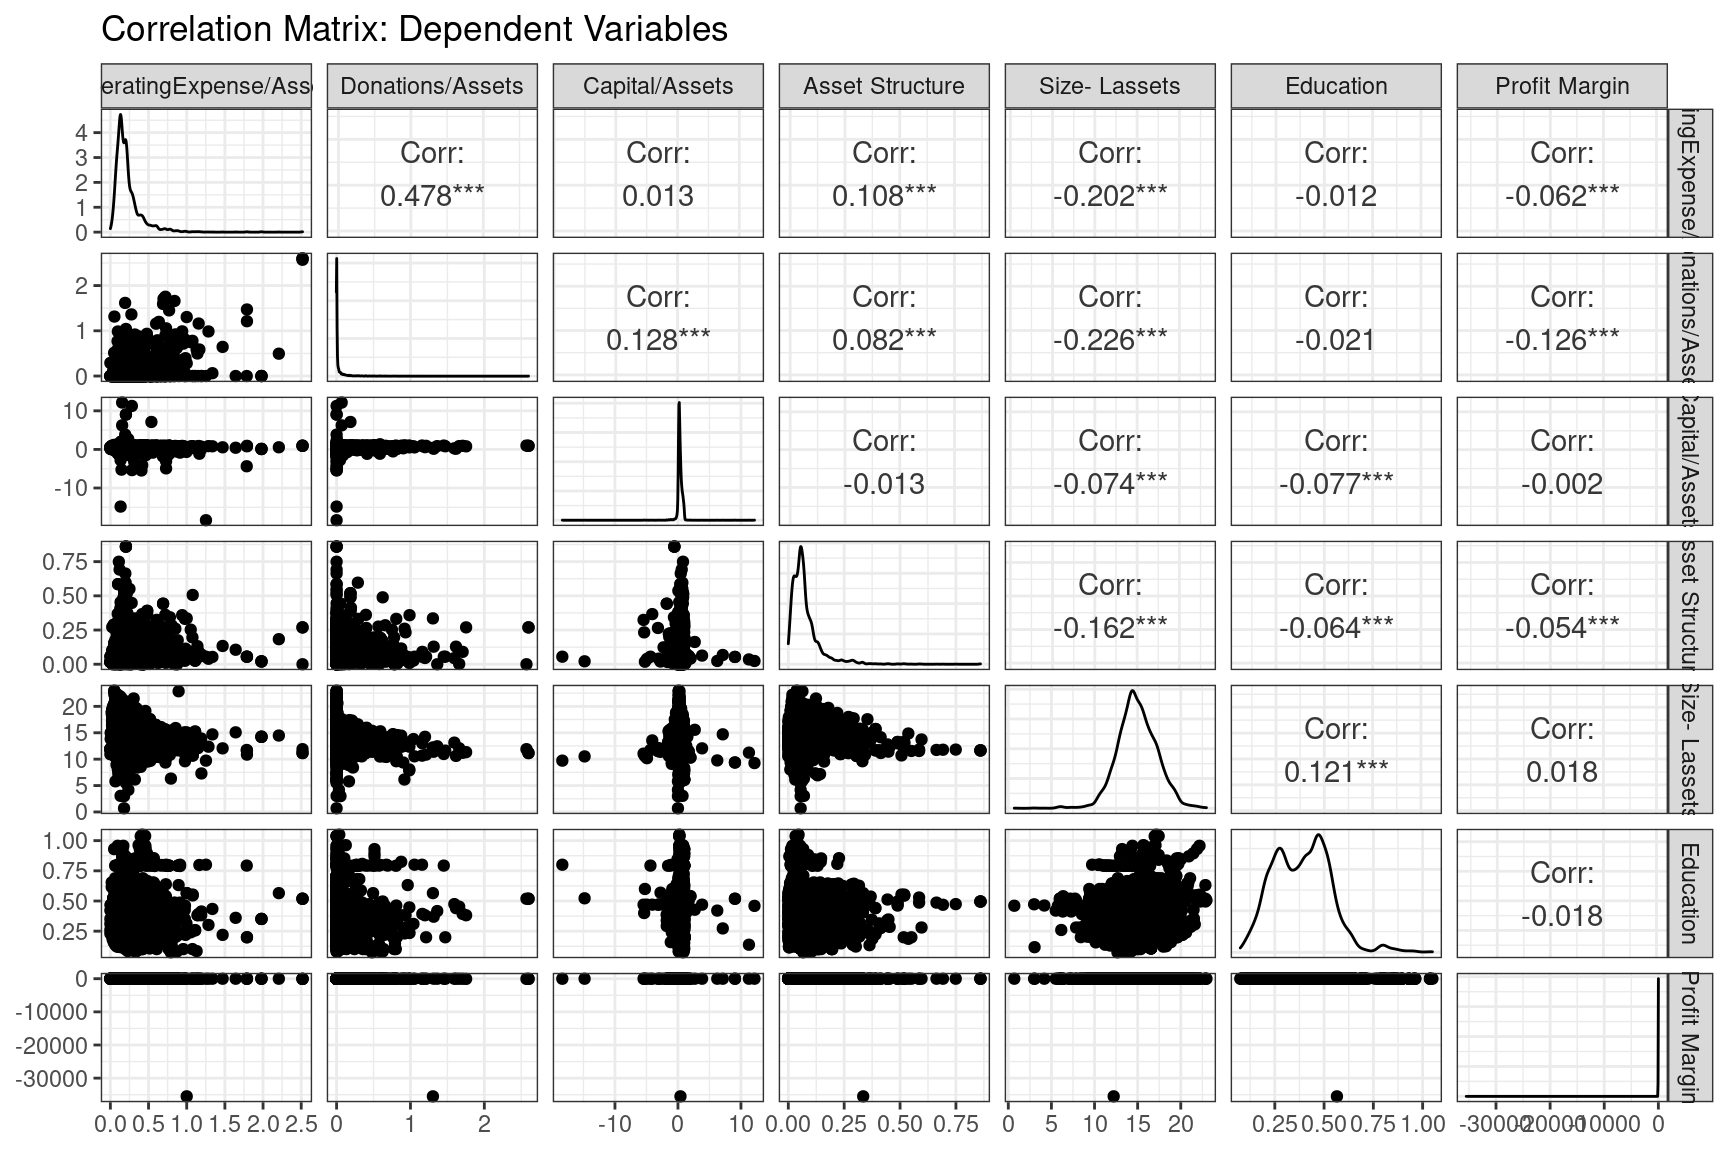
\includegraphics{04-tables_files/figure-latex/plots2-1.pdf}
\caption{\label{fig:plots2}Correlation Matrix for Independent Variables}
\end{figure}

\end{landscape}

Next, we visualise each of the numeric variables against the current legal forms (status) of MFIs. We use the median of the variables to stand for the variables. Figure 2 (Panel A) shows that mature MFIs form the bulk of MFIs in the sample. Among mature MFIs, NGOs and cooperatives are the majority, indicating their relatively longer operational cycle than NBFIs, banks, and rural banks. As expected, NGOs receive the highest share of donations, followed by credit unions and NBFIs, while commercial banks receive the least donations (Figure 2- Panel B). The result relating to NGOs is not surprising given they are rooted in the welfare model of microfinance. Most donors are likely to channel their funds to MFIs that place social performance over profits. When commercial capital almost entirely replaces donations, outreach to the poor may likely be affected \autocite{roberts2013profit}, given that managers may emphasise impressing shareholders and debt-holders in line with the agency theory. As noted by \textcite{d2013unsubsidized}, MFIs with little or no subsidies exhibit more significant mission drift. Hence, outreach to the poor would suffer even more where the capital providers do not have a sense of the hybrid nature of microfinance. Therefore, the rise of blended finance where commercial capital funds social causes may partly mitigate this scenario \autocite{attridge2019blended}.

Donations do not prevent NGOs and NBFIs from raising capital as they have the highest capital to assets ratio- which primarily reflects equity injections (Figure 2: Panel C). Commercial banks, credit unions and rural banks follow in that order. The observation is surprising given that NGOs and NBFIs still exhibit a high level of social performance even with a relatively high capital to assets feature. Therefore, it could imply that the profit vs social orientation of an MFI could be driven not just by the needs of the providers of funds but also by the internal governance, mission, and strategic direction of an MFI \autocite{campion1999institutional}. In this respect, an MFI's social mission could outweigh the needs of capital providers. Also, the equity capital NGOs may attract may be preferential in terms of expected returns, as with blended finance \autocite{rode2019blended}. In this case, donors could provide dedicated capital that does not pressure management to make high interest or dividends payments, allowing MFIs to remain predominantly on the social mission path \autocite{lopatta2016microfinance}. \footnote{Apart from credit unions/cooperatives and rural banks, we use acronyms for other legal forms of MFIs. NGO stands for non-governmental organisations, while NBFI connotes non-bank financial institutions. The term bank represents microfinance-oriented commercial banks.}

Appendix 10 and 11 show the visualisation for the debt to equity ratio and deposits to assets ratio. While NGOs attract more equity capital, rural banks, commercial banks, and credit unions rely more on debt, especially deposits form of debt, to finance their operations. The analysis shows that while all MFIs are raising capital, the sources are different for commercial MFIs vis-a-vis NGOs. While NGOs are inclined to using more equity, commercial MFIs appear to rely more on debt. Debt capital gives rise to fixed obligations that may exacerbate mission drift, and hence the conversion of NGOs to commercial entities could be harmful to social outreach. However, the relative inability to garner deposits maybe detrimental to NGOs' ability to access cheap, less restrictive capital.

Lastly, for asset structure (tangibility), the ratio of non-current assets to total assets, credit unions lead followed by commercial banks, NGOs, NBFIs, and rural banks. Asset structure captures the extent to which MFIs invest in physical infrastructure relative to the total asset base. Credit unions tend to serve a narrow geographic region and traditionally put up brick and mortar branches to serve their customers \autocite{mckillop2011credit}. Like credit unions, commercial banks tended to have more branches, having taken root before the advent of fintech, reducing the need for physical branches. NGOs, NBFIs, and rural banks have the lowest rates of asset tangibility, especially those of more recent origins, and using rural agents to meet customers rather than set up an expansive network of branches \autocite{kent2013bankers}.

Figure 3 (Panel A) shows that NGOs exhibit the highest median operating expense to assets ratio followed by NBFIs while credit unions trail. As we see later in the analysis, operating expenses positively relate to the depth of outreach- per cent of female borrowers and breadth of outreach in terms of gross loans to assets. Therefore, NGOs will do better in social outreach as they incur more costs to reach out to the financially excluded. Indeed, literature shows that outreach to the poor is expensive partly due to the dis-economies of scale in serving the poor, financially excluded clients \autocite{mia2017mission}. One of the efficiency enhancement opportunities from the transformation of MFIs to the for-profit approach to microfinance services delivery is that managers could trim operating expenses to increase profits hurting financial inclusion.

Turning to profitability in Figure 3 (Panel B), we find that rural and commercial banks post the highest median profits, while NBFIs and NGOs trail (Figure 3- Panel B). This result probably partially illustrates the emphasis on social performance over financial performance by the management. NGOs and NBFIs are more likely to favour the social goal. When we take this result together with the observation that NGOs tend to have more operating expenses, we conclude that the desire by managers of commercial banks and other for-profit MFIs to mitigate agency conflicts leads to less operating expenses, more profitability and, hence, lower outreach to the financially excluded \autocite{jensen1976theory}.

Overall, the pattern indicates that while NGOs spend the most in operating expenses to reach the financially excluded, these efforts come at the cost of profitability. In contrast, profit-oriented MFIs are keen to manage expenses that improve profitability, presumably at the expense of outreach to the financially excluded. It is worth noting that NGOs have a relatively low asset base and hold relatively fewer non-current assets to total assets. The observation could mean that NGOs do not invest heavily in brick and mortar branches or serve a relatively limited geographic range. Finally, NGOs have the highest capital (equity) to asset ratio despite the push towards commercial capital. Much could be from investors, who put forth dedicated equity capital because they are keen on social performance and not profits \autocite{mia2017mission}.

We now turn to Figure 4. The first graph (Figure 4- Panel A) shows that commercial banks have the most prominent asset size (total assets), while NGOs and cooperatives have the smallest in that order. Banks tend to have a much broader geographic presence and hence attract more clients, which means more assets accumulation. Again, capital adequacy requirements by central banks have implications on the assets that banks hold. Furthermore, commercial banks are generally dominant in many developing countries meaning that they have a long operating history which implies a bigger size \autocite{levine2002bank}. Figure 4 panel B shows that NGOs and NBFIs serve proportionately more women borrowers, indicating their outreach depth. Given that much of the donor funds accrues to NGOs, the conversion to the for-profit model would be detrimental to financial inclusion if coupled with a reduction in donor funding.

Commercial banks and credit unions have the highest average loan balance per borrower (depth of outreach), while NBFIs and NGOs come last in that order (Figure 4- Panel C). As an indicator of outreach to the poor, the average loan balance per borrower is better when lower, indicating that more impoverished people get access to financial services. Again, it appears that profit-orientation by commercial banks may cause MFIs to reach less financially excluded people in favour of making profits. For credit unions, the observation could arise due to the limited geographic range of operations where they serve people with a common interest like the type of occupation, meaning that their members may not be suffering from financial exclusion in the first place \autocite{armendariz2013subsidy}.

NGOs have the highest median gross loans to total assets ratio, surprising given their relatively smaller size. On the other hand, banks and rural banks, respectively, have the lowest gross loans to assets, meaning they are less efficient in converting their assets into credit (Figure 4- Panel D). Again, it shows, at least in the case of Africa, that the breadth and depth of financial outreach are not always mutually exclusive. In this case, NGOs can reach the most impoverished borrowers, going by the per cent of female borrowers and average loan balance per borrower, while at the same time seemingly reaching a broad customer base as indicated by the gross loans to assets. So far, the bulk of MFIs population leans towards the welfare orientation where profitability overtly seems incompatible with outreach to the financially excluded \autocite{lopatta2016microfinance}.

\newpage
\begin{landscape}

\begin{Shaded}
\begin{Highlighting}[]
\NormalTok{box1 }\OtherTok{\textless{}{-}}\NormalTok{ my\_data }\SpecialCharTok{\%\textgreater{}\%} \FunctionTok{ggplot}\NormalTok{(}\FunctionTok{aes}\NormalTok{(}\AttributeTok{x =}\NormalTok{ age, }\AttributeTok{fill =}\NormalTok{ currentlegalstatus)) }\SpecialCharTok{+} 
  
  \FunctionTok{geom\_bar}\NormalTok{() }\SpecialCharTok{+} \FunctionTok{labs}\NormalTok{(}\AttributeTok{x =} \StringTok{"Age"}\NormalTok{, }\AttributeTok{y =} \StringTok{"Count"}\NormalTok{)}


\NormalTok{box2 }\OtherTok{\textless{}{-}} \FunctionTok{second\_plotter}\NormalTok{(}\AttributeTok{data =}\NormalTok{ my\_data, }\AttributeTok{x =}\NormalTok{ currentlegalstatus, }
        \AttributeTok{z =}\NormalTok{ currentlegalstatus,}
        \AttributeTok{y =}\NormalTok{ donations\_assets\_ratio, }
        \AttributeTok{xlabel =} \StringTok{"Current Legal Status"}\NormalTok{, }
        \AttributeTok{ylabel =} \StringTok{"Donations/Assets Ratio (log Scale)"}\NormalTok{, }
        \AttributeTok{title =} \StringTok{"Panel B: Donations to Assets Ratio by MFIs Legal Status"}\NormalTok{)}
\end{Highlighting}
\end{Shaded}

\begin{verbatim}
## Warning: `guides(<scale> = FALSE)` is deprecated. Please use `guides(<scale> =
## "none")` instead.
\end{verbatim}

\begin{Shaded}
\begin{Highlighting}[]
\NormalTok{box3 }\OtherTok{\textless{}{-}} \FunctionTok{second\_plotter}\NormalTok{(}\AttributeTok{data =}\NormalTok{ my\_data, }\AttributeTok{x =}\NormalTok{ currentlegalstatus, }
        \AttributeTok{z =}\NormalTok{ currentlegalstatus,}
        \AttributeTok{y =}\NormalTok{ capital\_asset\_ratio, }
        \AttributeTok{xlabel =} \StringTok{"Current Legal Status"}\NormalTok{, }
        \AttributeTok{ylabel =} \StringTok{"Capital/Assets Ratio (log Scale)"}\NormalTok{, }
        \AttributeTok{title =} \StringTok{"Panel C: Capital to Assets Ratio by MFIs Legal Status"}\NormalTok{)}
\end{Highlighting}
\end{Shaded}

\begin{verbatim}
## Warning: `guides(<scale> = FALSE)` is deprecated. Please use `guides(<scale> =
## "none")` instead.
\end{verbatim}

\begin{Shaded}
\begin{Highlighting}[]
\NormalTok{box4 }\OtherTok{\textless{}{-}} \FunctionTok{second\_plotter}\NormalTok{(}\AttributeTok{data =}\NormalTok{ my\_data, }\AttributeTok{x =}\NormalTok{ currentlegalstatus, }
        \AttributeTok{z =}\NormalTok{ currentlegalstatus,}
        \AttributeTok{y =}\NormalTok{ asset\_structure, }
        \AttributeTok{xlabel =} \StringTok{"Current Legal Status"}\NormalTok{, }
        \AttributeTok{ylabel =} \StringTok{"Asset Structure (log Scale)"}\NormalTok{, }
        \AttributeTok{title =} \StringTok{"Panel D: Asset Structure of MFIs by MFI Legal Status"}\NormalTok{)}
\end{Highlighting}
\end{Shaded}

\begin{verbatim}
## Warning: `guides(<scale> = FALSE)` is deprecated. Please use `guides(<scale> =
## "none")` instead.
\end{verbatim}

\begin{Shaded}
\begin{Highlighting}[]
\FunctionTok{library}\NormalTok{(patchwork)}
\NormalTok{(box1 }\SpecialCharTok{+}\NormalTok{ box2) }\SpecialCharTok{/}\NormalTok{ (box3 }\SpecialCharTok{+}\NormalTok{ box4) }\SpecialCharTok{+} \FunctionTok{plot\_annotation}\NormalTok{(}\AttributeTok{title =} \StringTok{""}\NormalTok{, }\AttributeTok{caption =} \StringTok{"Source: Authors\textquotesingle{} construction from MIX Data. NB: The y{-}Axis is in log scale"}\NormalTok{)}
\end{Highlighting}
\end{Shaded}

\begin{verbatim}
## Warning in self$trans$transform(x): NaNs produced
\end{verbatim}

\begin{verbatim}
## Warning: Transformation introduced infinite values in continuous y-axis
\end{verbatim}

\begin{verbatim}
## Warning in self$trans$transform(x): NaNs produced
\end{verbatim}

\begin{verbatim}
## Warning: Transformation introduced infinite values in continuous y-axis
\end{verbatim}

\begin{verbatim}
## Warning in self$trans$transform(x): NaNs produced
\end{verbatim}

\begin{verbatim}
## Warning: Transformation introduced infinite values in continuous y-axis
\end{verbatim}

\begin{verbatim}
## Warning: Removed 2038 rows containing non-finite values (stat_ydensity).
\end{verbatim}

\begin{verbatim}
## Warning: Removed 2038 rows containing non-finite values (stat_boxplot).
\end{verbatim}

\begin{verbatim}
## Warning: Removed 2038 rows containing missing values (geom_point).
\end{verbatim}

\begin{verbatim}
## Warning in self$trans$transform(x): NaNs produced
\end{verbatim}

\begin{verbatim}
## Warning: Transformation introduced infinite values in continuous y-axis
\end{verbatim}

\begin{verbatim}
## Warning in self$trans$transform(x): NaNs produced
\end{verbatim}

\begin{verbatim}
## Warning: Transformation introduced infinite values in continuous y-axis
\end{verbatim}

\begin{verbatim}
## Warning in self$trans$transform(x): NaNs produced
\end{verbatim}

\begin{verbatim}
## Warning: Transformation introduced infinite values in continuous y-axis
\end{verbatim}

\begin{verbatim}
## Warning: Removed 252 rows containing non-finite values (stat_ydensity).
\end{verbatim}

\begin{verbatim}
## Warning: Removed 252 rows containing non-finite values (stat_boxplot).
\end{verbatim}

\begin{verbatim}
## Warning: Removed 252 rows containing missing values (geom_point).
\end{verbatim}

\begin{verbatim}
## Warning: Transformation introduced infinite values in continuous y-axis

## Warning: Transformation introduced infinite values in continuous y-axis

## Warning: Transformation introduced infinite values in continuous y-axis
\end{verbatim}

\begin{verbatim}
## Warning: Removed 21 rows containing non-finite values (stat_ydensity).
\end{verbatim}

\begin{verbatim}
## Warning: Removed 21 rows containing non-finite values (stat_boxplot).
\end{verbatim}

\begin{verbatim}
## Warning: Removed 21 rows containing missing values (geom_point).
\end{verbatim}

\begin{figure}
\centering
\includegraphics{04-tables_files/figure-latex/unnamed-chunk-13-1.pdf}
\caption{\label{fig:unnamed-chunk-13}Operating Expense, Donations, Capital and Asset Structure of MFIs by Legal Status}
\end{figure}

\newpage

\begin{Shaded}
\begin{Highlighting}[]
\NormalTok{box9 }\OtherTok{\textless{}{-}} \FunctionTok{second\_plotter}\NormalTok{(}\AttributeTok{data =}\NormalTok{ my\_data, }\AttributeTok{x =}\NormalTok{ currentlegalstatus, }
        \AttributeTok{z =}\NormalTok{ currentlegalstatus,}
        \AttributeTok{y =}\NormalTok{ my\_data}\SpecialCharTok{$}\NormalTok{operating\_expense\_assets, }
        \AttributeTok{xlabel =} \StringTok{"Current Legal Status"}\NormalTok{, }
        \AttributeTok{ylabel =} \StringTok{"Opareting Expense to Assets (log Scale)"}\NormalTok{, }
        \AttributeTok{title =} \StringTok{"Panel A: Operating Expense to Assets Ratio of MFIs by MFI Legal Status"}\NormalTok{)}
\end{Highlighting}
\end{Shaded}

\begin{verbatim}
## Warning: `guides(<scale> = FALSE)` is deprecated. Please use `guides(<scale> =
## "none")` instead.
\end{verbatim}

\begin{Shaded}
\begin{Highlighting}[]
\NormalTok{box10 }\OtherTok{\textless{}{-}} \FunctionTok{second\_plotter}\NormalTok{(}\AttributeTok{data =}\NormalTok{ my\_data, }\AttributeTok{x =}\NormalTok{ currentlegalstatus, }
        \AttributeTok{z =}\NormalTok{ currentlegalstatus,}
        \AttributeTok{y =}\NormalTok{ profit\_margin, }
        \AttributeTok{xlabel =} \StringTok{"Current Legal Status"}\NormalTok{, }
        \AttributeTok{ylabel =} \StringTok{"Profit Margin (log Scale)"}\NormalTok{, }
        \AttributeTok{title =} \StringTok{"Panel B: Profit Margin by MFIs Legal Status"}\NormalTok{)}
\end{Highlighting}
\end{Shaded}

\begin{verbatim}
## Warning: `guides(<scale> = FALSE)` is deprecated. Please use `guides(<scale> =
## "none")` instead.
\end{verbatim}

\begin{Shaded}
\begin{Highlighting}[]
\FunctionTok{library}\NormalTok{(patchwork)}

\NormalTok{(box9 }\SpecialCharTok{+}\NormalTok{ box10) }\SpecialCharTok{+} \FunctionTok{plot\_annotation}\NormalTok{(}\AttributeTok{title =} \StringTok{""}\NormalTok{, }\AttributeTok{caption =} \StringTok{"Source: Authors\textquotesingle{} construction from MIX Data }\SpecialCharTok{\textbackslash{}n}
\StringTok{                                                The y{-}Axis is in log scale"}\NormalTok{)}
\end{Highlighting}
\end{Shaded}

\begin{verbatim}
## Warning: Use of `my_data$operating_expense_assets` is discouraged. Use
## `operating_expense_assets` instead.
\end{verbatim}

\begin{verbatim}
## Warning: Use of `my_data$operating_expense_assets` is discouraged. Use
## `operating_expense_assets` instead.

## Warning: Use of `my_data$operating_expense_assets` is discouraged. Use
## `operating_expense_assets` instead.

## Warning: Use of `my_data$operating_expense_assets` is discouraged. Use
## `operating_expense_assets` instead.

## Warning: Use of `my_data$operating_expense_assets` is discouraged. Use
## `operating_expense_assets` instead.

## Warning: Use of `my_data$operating_expense_assets` is discouraged. Use
## `operating_expense_assets` instead.
\end{verbatim}

\begin{verbatim}
## Warning: Transformation introduced infinite values in continuous y-axis

## Warning: Transformation introduced infinite values in continuous y-axis

## Warning: Transformation introduced infinite values in continuous y-axis
\end{verbatim}

\begin{verbatim}
## Warning: Removed 5 rows containing non-finite values (stat_ydensity).
\end{verbatim}

\begin{verbatim}
## Warning: Removed 5 rows containing non-finite values (stat_boxplot).
\end{verbatim}

\begin{verbatim}
## Warning: Removed 5 rows containing missing values (geom_point).
\end{verbatim}

\begin{verbatim}
## Warning in self$trans$transform(x): NaNs produced
\end{verbatim}

\begin{verbatim}
## Warning: Transformation introduced infinite values in continuous y-axis
\end{verbatim}

\begin{verbatim}
## Warning in self$trans$transform(x): NaNs produced
\end{verbatim}

\begin{verbatim}
## Warning: Transformation introduced infinite values in continuous y-axis
\end{verbatim}

\begin{verbatim}
## Warning in self$trans$transform(x): NaNs produced
\end{verbatim}

\begin{verbatim}
## Warning: Transformation introduced infinite values in continuous y-axis
\end{verbatim}

\begin{verbatim}
## Warning: Removed 1794 rows containing non-finite values (stat_ydensity).
\end{verbatim}

\begin{verbatim}
## Warning: Removed 1794 rows containing non-finite values (stat_boxplot).
\end{verbatim}

\begin{verbatim}
## Warning: Removed 1794 rows containing missing values (geom_point).
\end{verbatim}

\begin{figure}
\centering
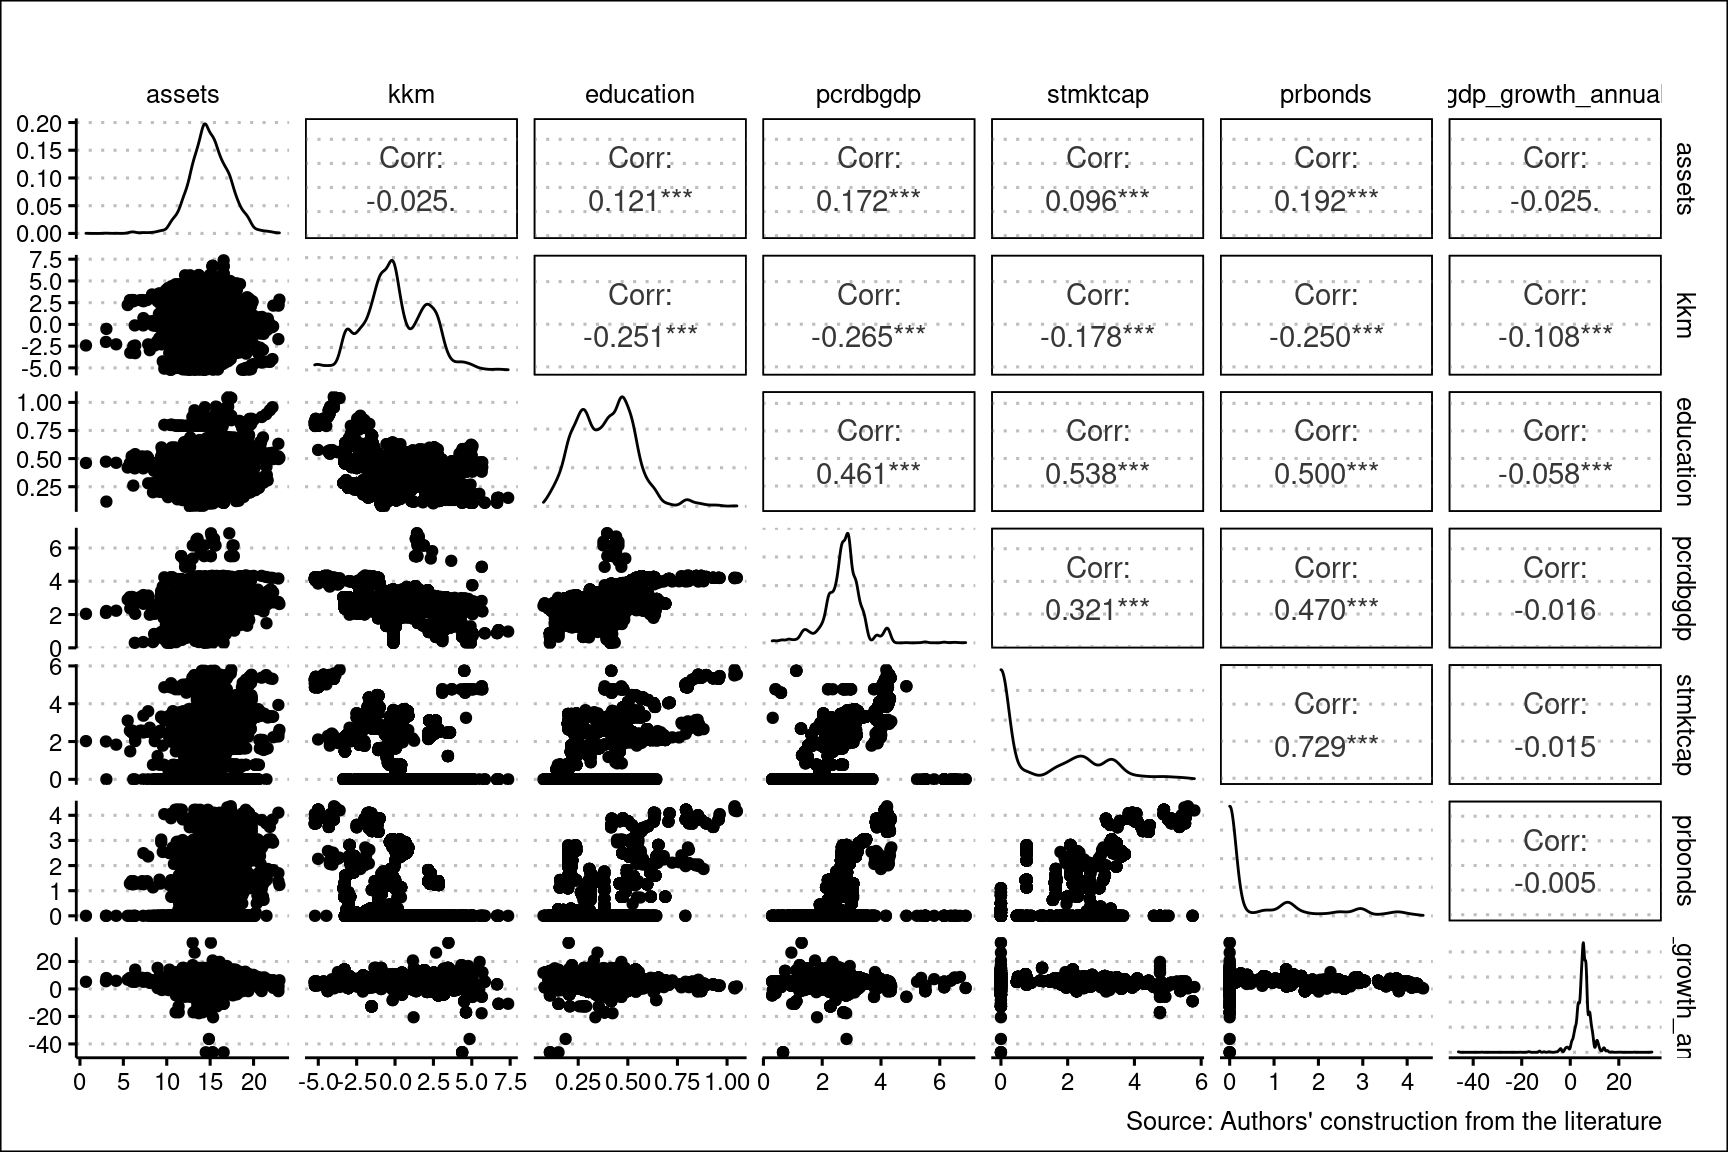
\includegraphics{04-tables_files/figure-latex/unnamed-chunk-14-1.pdf}
\caption{\label{fig:unnamed-chunk-14}Asset Structure, Profit Margin, Donations, Capital to Assets Ratio by Current Legal Status}
\end{figure}

\end{landscape}

\newpage
\begin{landscape}

\begin{Shaded}
\begin{Highlighting}[]
\NormalTok{box5 }\OtherTok{\textless{}{-}} \FunctionTok{second\_plotter}\NormalTok{(}\AttributeTok{data =}\NormalTok{ my\_data, }\AttributeTok{x =}\NormalTok{ currentlegalstatus, }
        \AttributeTok{z =}\NormalTok{ currentlegalstatus,}
        \AttributeTok{y =}\NormalTok{ assets, }
        \AttributeTok{xlabel =} \StringTok{"Current Legal Status"}\NormalTok{, }
        \AttributeTok{ylabel =} \StringTok{"Size {-} Log of Total Assets (log Scale)"}\NormalTok{, }
        \AttributeTok{title =} \StringTok{"Panel A: Relative Size of MFIs by MFI Legal Status"}\NormalTok{)}
\end{Highlighting}
\end{Shaded}

\begin{verbatim}
## Warning: `guides(<scale> = FALSE)` is deprecated. Please use `guides(<scale> =
## "none")` instead.
\end{verbatim}

\begin{Shaded}
\begin{Highlighting}[]
\NormalTok{box6 }\OtherTok{\textless{}{-}} \FunctionTok{second\_plotter}\NormalTok{(}\AttributeTok{data =}\NormalTok{ my\_data, }\AttributeTok{x =}\NormalTok{ currentlegalstatus, }
        \AttributeTok{z =}\NormalTok{ currentlegalstatus,}
        \AttributeTok{y =}\NormalTok{ percent\_of\_female\_borrowers, }
        \AttributeTok{xlabel =} \StringTok{"Current Legal Status"}\NormalTok{, }
        \AttributeTok{ylabel =} \StringTok{"Percent of Female Borrowers (log Scale)"}\NormalTok{, }
        \AttributeTok{title =} \StringTok{"Panel B: Percent of Female Borrowers by MFIs Legal Status"}\NormalTok{)}
\end{Highlighting}
\end{Shaded}

\begin{verbatim}
## Warning: `guides(<scale> = FALSE)` is deprecated. Please use `guides(<scale> =
## "none")` instead.
\end{verbatim}

\begin{Shaded}
\begin{Highlighting}[]
\NormalTok{box7 }\OtherTok{\textless{}{-}} \FunctionTok{second\_plotter}\NormalTok{(}\AttributeTok{data =}\NormalTok{ my\_data, }\AttributeTok{x =}\NormalTok{ currentlegalstatus, }
        \AttributeTok{z =}\NormalTok{ currentlegalstatus,}
        \AttributeTok{y =}\NormalTok{ average\_loan\_balance\_per\_borrower, }
        \AttributeTok{xlabel =} \StringTok{"Current Legal Status"}\NormalTok{, }
        \AttributeTok{ylabel =} \StringTok{"Loan Balance per Borrower (log Scale)"}\NormalTok{, }
        \AttributeTok{title =} \StringTok{"Panel C: Loan Balance per Borrower by MFIs Legal Status"}\NormalTok{)}
\end{Highlighting}
\end{Shaded}

\begin{verbatim}
## Warning: `guides(<scale> = FALSE)` is deprecated. Please use `guides(<scale> =
## "none")` instead.
\end{verbatim}

\begin{Shaded}
\begin{Highlighting}[]
\NormalTok{box8 }\OtherTok{\textless{}{-}} \FunctionTok{second\_plotter}\NormalTok{(}\AttributeTok{data =}\NormalTok{ my\_data, }\AttributeTok{x =}\NormalTok{ currentlegalstatus, }
        \AttributeTok{z =}\NormalTok{ currentlegalstatus,}
        \AttributeTok{y =}\NormalTok{ gross\_loan\_portfolio\_to\_total\_assets, }
        \AttributeTok{xlabel =} \StringTok{"Current Legal Status"}\NormalTok{, }
        \AttributeTok{ylabel =} \StringTok{"Gross Loans/ Assets (log Scale)"}\NormalTok{, }
        \AttributeTok{title =} \StringTok{"Panel D: Gross Loans to Assets by MFIs Legal Status"}\NormalTok{)}
\end{Highlighting}
\end{Shaded}

\begin{verbatim}
## Warning: `guides(<scale> = FALSE)` is deprecated. Please use `guides(<scale> =
## "none")` instead.
\end{verbatim}

\begin{Shaded}
\begin{Highlighting}[]
\FunctionTok{library}\NormalTok{(patchwork)}

\NormalTok{(box5 }\SpecialCharTok{+}\NormalTok{ box6)}\SpecialCharTok{/}\NormalTok{ (box7 }\SpecialCharTok{+}\NormalTok{ box8) }\SpecialCharTok{+} \FunctionTok{plot\_annotation}\NormalTok{(}\AttributeTok{title =} \StringTok{""}\NormalTok{, }\AttributeTok{caption =} \StringTok{"Source: Authors\textquotesingle{} construction from MIX Data }\SpecialCharTok{\textbackslash{}n}
\StringTok{                                                The y{-}Axis is in log scale"}\NormalTok{)}
\end{Highlighting}
\end{Shaded}

\begin{verbatim}
## Warning: Transformation introduced infinite values in continuous y-axis
\end{verbatim}

\begin{verbatim}
## Warning: Transformation introduced infinite values in continuous y-axis

## Warning: Transformation introduced infinite values in continuous y-axis
\end{verbatim}

\begin{verbatim}
## Warning: Removed 12 rows containing non-finite values (stat_ydensity).
\end{verbatim}

\begin{verbatim}
## Warning: Removed 12 rows containing non-finite values (stat_boxplot).
\end{verbatim}

\begin{verbatim}
## Warning: Removed 12 rows containing missing values (geom_point).
\end{verbatim}

\begin{verbatim}
## Warning: Transformation introduced infinite values in continuous y-axis

## Warning: Transformation introduced infinite values in continuous y-axis

## Warning: Transformation introduced infinite values in continuous y-axis
\end{verbatim}

\begin{verbatim}
## Warning: Removed 322 rows containing non-finite values (stat_ydensity).
\end{verbatim}

\begin{verbatim}
## Warning: Removed 322 rows containing non-finite values (stat_boxplot).
\end{verbatim}

\begin{verbatim}
## Warning: Removed 322 rows containing missing values (geom_point).
\end{verbatim}

\begin{verbatim}
## Warning: Transformation introduced infinite values in continuous y-axis

## Warning: Transformation introduced infinite values in continuous y-axis

## Warning: Transformation introduced infinite values in continuous y-axis
\end{verbatim}

\begin{verbatim}
## Warning: Removed 128 rows containing non-finite values (stat_ydensity).
\end{verbatim}

\begin{verbatim}
## Warning: Removed 128 rows containing non-finite values (stat_boxplot).
\end{verbatim}

\begin{verbatim}
## Warning: Removed 128 rows containing missing values (geom_point).
\end{verbatim}

\begin{figure}
\centering
\includegraphics{04-tables_files/figure-latex/unnamed-chunk-15-1.pdf}
\caption{\label{fig:unnamed-chunk-15}Size, Profit Margin, Average Loan Balance per Borrower and Gross of MFIs by Legal Status}
\end{figure}

\end{landscape}
\newpage

\hypertarget{trends-in-dependent-and-independent-variables}{%
\subsubsection{\texorpdfstring{\textbf{Trends in Dependent and Independent Variables}}{Trends in Dependent and Independent Variables}}\label{trends-in-dependent-and-independent-variables}}

Figure 4 below maps the trends, over time, for donations, capital, profits and operating expense to assets ratio, respectively. Figure 5 (\emph{Panel A}) shows that the median donations to assets ratio have been downward for 1999-2019. The observation confirms the neo-liberal shift in the MFI paradigm where donors expect MFIs to be more financially self-sustainable. The trend is expected in light of the abundance of literature on the conversion of MFIs from NGOs and subsequent drop in donor funding \autocite{d2017ngos}. As donations dry up, we expect the debt and equity capital components to fill the void.

Surprisingly, the capital to assets ratio, which captures the extent of the equity capital injection, is also on a downward trend despite the drive towards the commercialization of MFIs (\emph{Figure 5, Panel B}). The observation could be due to a rise in the total asset base of MFIs, as they scale up, with equity capital being a relatively smaller external capital component than debt. \emph{Appendix 8} shows a steady increase in the debt/equity ratio, which means that most MFIs, like commercial banks, use debt (including deposits) to finance their operations. In this respect, debt gives rise to fixed obligations which could hurt profitability during economic downturns.

MFI profitability in Figure 5 (\emph{Panel C}) shows that the median profitability for MFIs is meager and almost invariant over time, except *for a significant dip in mean profitability around 2008-2009 during the global financial crisis period. The result is consistent with the empirical regularity that shows microfinance as a low margin business, largely reflecting the primacy of social mission in microfinance \autocite{hartarska2012governance}. An important observation is that there are no distinctive profitability changes even as more MFIs adopt the commercial model. This observation means that either the commercialization was not very successful in generating profits or that the extent to which MFIs were able to make profits post-transformation is particularly peculiar to each MFI or to each of the legal forms of MFIs.

Lastly, for Figure 5 (\emph{Panel D}), the operating expenses to assets ratio remains approximately constant except for a dip in the 1999-2001 period. As the regressions show in a later section, the operating expense to assets ratio relates positively to outreach depth and breadth. In this case, the drop in the ratio between 1999 and 2001 could have worsened financial inclusion outcomes. However, the operating expenses to assets ratio have levelled off; thus, it could be indicating a sustained commitment to outreach even in the face of the desire to make profits.

Next, we turn to Figure 6, which shows a rise in MFI size, average loan balance per borrower, and gross loans to total assets, while the per cent of female borrowers is on a downward trend. The rise in the average loan's balance per borrower and the accompanying drop in the proportion of female borrowers indicates a consistent decline in the outreach of MFIs to the financially excluded, as MFIs rely less on donations and more on commercial capital. It further shows the effects of the neo-liberal, for-profit paradigm, which may be hurting the social performance of MFIs, precisely the depth of outreach. However, it appears the breadth of outreach is getting better with time as MFIs give more loans. Taken together, it implies that MFIs provide larger loans to less financially excluded people in a bid to make ample financial return to allow for financial sustainability and payment of dividends and interest to investors.

Appendices 12-14 show the breakdown, by legal forms of MFIs, of the trends for per cent of female borrowers, average loan balance per borrower and gross loans to assets. The movement is generally downwards for women borrowers except under the commercial banking legal forms, which have low outreach to women, but that is relatively constant after the initial spike in the early 2000s. The trends indicate a weakening depth of outreach. For average loan balance per borrower, NGOs and rural banks remain relatively constant. At the same time, other legal forms have rising average loan size trends, which indicates worsening outreach by banks, credit unions, and NBFIs. Lastly, gross loans are rising except for rural banks, showing a better breadth of outreach over time.

\begin{Shaded}
\begin{Highlighting}[]
\DocumentationTok{\#\# Percent of female borrowers {-} trends over time}
\NormalTok{female }\OtherTok{\textless{}{-}}\NormalTok{ my\_data }\SpecialCharTok{\%\textgreater{}\%} 
  
  \FunctionTok{group\_by}\NormalTok{(year) }\SpecialCharTok{\%\textgreater{}\%} 
  
  \FunctionTok{summarize}\NormalTok{(}\AttributeTok{mean\_female =} \FunctionTok{mean}\NormalTok{(percent\_of\_female\_borrowers, }\AttributeTok{na.rm =} \ConstantTok{TRUE}\NormalTok{), }
                               
  \AttributeTok{median\_female =} \FunctionTok{median}\NormalTok{(percent\_of\_female\_borrowers, }\AttributeTok{na.rm =} \ConstantTok{TRUE}\NormalTok{)) }\SpecialCharTok{\%\textgreater{}\%} 
  
  \FunctionTok{ggplot}\NormalTok{(}\AttributeTok{mapping =} \FunctionTok{aes}\NormalTok{(}\AttributeTok{x =}\NormalTok{ year, }\AttributeTok{y =}\NormalTok{ mean\_female), }\AttributeTok{color =} \StringTok{"skyblue"}\NormalTok{) }\SpecialCharTok{+} \FunctionTok{geom\_line}\NormalTok{() }\SpecialCharTok{+}
  
  \FunctionTok{geom\_line}\NormalTok{(}\AttributeTok{mapping =} \FunctionTok{aes}\NormalTok{(}\AttributeTok{x =}\NormalTok{ year, }\AttributeTok{y =}\NormalTok{ median\_female), }\AttributeTok{linetype =} \StringTok{"dashed"}\NormalTok{, }\AttributeTok{color =} \StringTok{"red"}\NormalTok{) }\SpecialCharTok{+}
  
  \FunctionTok{geom\_text}\NormalTok{(}\AttributeTok{x =} \DecValTok{2018}\NormalTok{, }\AttributeTok{y =} \FloatTok{0.55}\NormalTok{, }\AttributeTok{label =} \StringTok{"Median"}\NormalTok{) }\SpecialCharTok{+} 
  
  \FunctionTok{geom\_text}\NormalTok{(}\AttributeTok{x =} \DecValTok{2018}\NormalTok{, }\AttributeTok{y =} \FloatTok{0.57}\NormalTok{, }\AttributeTok{label =} \StringTok{"Mean"}\NormalTok{)}\SpecialCharTok{+}
  
  \FunctionTok{labs}\NormalTok{(}\AttributeTok{x =} \StringTok{"Year"}\NormalTok{, }\AttributeTok{y =} \StringTok{"Mean/Median Percent of Female Borrowers"}\NormalTok{, }\AttributeTok{title =} \StringTok{"Panel B: Trends in the Percent of Female Borrowers"}\NormalTok{) }\SpecialCharTok{+} 
  
\NormalTok{  ggthemes}\SpecialCharTok{::}\FunctionTok{theme\_clean}\NormalTok{()}

\DocumentationTok{\#\# Average loan Balance per borrower}
\NormalTok{avloan }\OtherTok{\textless{}{-}}\NormalTok{ my\_data }\SpecialCharTok{\%\textgreater{}\%} 
  
  \FunctionTok{group\_by}\NormalTok{(year) }\SpecialCharTok{\%\textgreater{}\%} 
  
  \FunctionTok{summarize}\NormalTok{(}\AttributeTok{mean\_average\_loan =} \FunctionTok{mean}\NormalTok{(average\_loan\_balance\_per\_borrower, }\AttributeTok{na.rm =} \ConstantTok{TRUE}\NormalTok{), }
                               
  \AttributeTok{median\_average\_loan =} \FunctionTok{median}\NormalTok{(average\_loan\_balance\_per\_borrower, }\AttributeTok{na.rm =} \ConstantTok{TRUE}\NormalTok{)) }\SpecialCharTok{\%\textgreater{}\%} 
  
  \FunctionTok{ggplot}\NormalTok{(}\AttributeTok{mapping =} \FunctionTok{aes}\NormalTok{(}\AttributeTok{x =}\NormalTok{ year, }\AttributeTok{y =}\NormalTok{ mean\_average\_loan), }\AttributeTok{color =} \StringTok{"skyblue"}\NormalTok{) }\SpecialCharTok{+} \FunctionTok{geom\_line}\NormalTok{() }\SpecialCharTok{+}
  
  \FunctionTok{geom\_line}\NormalTok{(}\AttributeTok{mapping =} \FunctionTok{aes}\NormalTok{(}\AttributeTok{x =}\NormalTok{ year, }\AttributeTok{y =}\NormalTok{ median\_average\_loan), }\AttributeTok{linetype =} \StringTok{"dashed"}\NormalTok{, }\AttributeTok{color =} \StringTok{"red"}\NormalTok{) }\SpecialCharTok{+}
  
  \FunctionTok{geom\_text}\NormalTok{(}\AttributeTok{x =} \DecValTok{2018}\NormalTok{, }\AttributeTok{y =} \DecValTok{500}\NormalTok{, }\AttributeTok{label =} \StringTok{"Median"}\NormalTok{) }\SpecialCharTok{+} 
  
  \FunctionTok{geom\_text}\NormalTok{(}\AttributeTok{x =} \DecValTok{2016}\NormalTok{, }\AttributeTok{y =} \DecValTok{1200}\NormalTok{, }\AttributeTok{label =} \StringTok{"Mean"}\NormalTok{)}\SpecialCharTok{+}
  
  \FunctionTok{labs}\NormalTok{(}\AttributeTok{x =} \StringTok{"Year"}\NormalTok{, }\AttributeTok{y =} \StringTok{"Mean/Median Average Loan Balance per Borrower"}\NormalTok{, }\AttributeTok{title =} \StringTok{"Panel C: Trends in Average Loan Balance per Borrower"}\NormalTok{) }\SpecialCharTok{+} 
  
\NormalTok{  ggthemes}\SpecialCharTok{::}\FunctionTok{theme\_clean}\NormalTok{()}


\DocumentationTok{\#\# Gross loan portfolio to assets }
\NormalTok{grossloan }\OtherTok{\textless{}{-}}\NormalTok{ my\_data }\SpecialCharTok{\%\textgreater{}\%} 
  
  \FunctionTok{group\_by}\NormalTok{(year) }\SpecialCharTok{\%\textgreater{}\%} 
  
  \FunctionTok{summarize}\NormalTok{(}\AttributeTok{mean\_gross\_loans =} \FunctionTok{mean}\NormalTok{(gross\_loan\_portfolio\_to\_total\_assets, }\AttributeTok{na.rm =} \ConstantTok{TRUE}\NormalTok{), }
                               
  \AttributeTok{median\_gross\_loans =} \FunctionTok{median}\NormalTok{(gross\_loan\_portfolio\_to\_total\_assets, }\AttributeTok{na.rm =} \ConstantTok{TRUE}\NormalTok{)) }\SpecialCharTok{\%\textgreater{}\%} 
  
  \FunctionTok{ggplot}\NormalTok{(}\AttributeTok{mapping =} \FunctionTok{aes}\NormalTok{(}\AttributeTok{x =}\NormalTok{ year, }\AttributeTok{y =}\NormalTok{ mean\_gross\_loans), }\AttributeTok{color =} \StringTok{"skyblue"}\NormalTok{) }\SpecialCharTok{+} \FunctionTok{geom\_line}\NormalTok{() }\SpecialCharTok{+}
  
  \FunctionTok{geom\_line}\NormalTok{(}\AttributeTok{mapping =} \FunctionTok{aes}\NormalTok{(}\AttributeTok{x =}\NormalTok{ year, }\AttributeTok{y =}\NormalTok{ median\_gross\_loans), }\AttributeTok{linetype =} \StringTok{"dashed"}\NormalTok{, }\AttributeTok{color =} \StringTok{"red"}\NormalTok{) }\SpecialCharTok{+}
  
  \FunctionTok{geom\_text}\NormalTok{(}\AttributeTok{x =} \DecValTok{2012}\NormalTok{, }\AttributeTok{y =} \FloatTok{0.64}\NormalTok{, }\AttributeTok{label =} \StringTok{"Median"}\NormalTok{) }\SpecialCharTok{+} 
  
  \FunctionTok{geom\_text}\NormalTok{(}\AttributeTok{x =} \DecValTok{2013}\NormalTok{, }\AttributeTok{y =} \FloatTok{0.7}\NormalTok{, }\AttributeTok{label =} \StringTok{"Mean"}\NormalTok{)}\SpecialCharTok{+}
  
  \FunctionTok{labs}\NormalTok{(}\AttributeTok{x =} \StringTok{"Year"}\NormalTok{, }\AttributeTok{y =} \StringTok{"Mean/Median Gross Loans to Assets"}\NormalTok{, }\AttributeTok{title =} \StringTok{"Panel D: Trends in Gross Loans to Assets Ratio"}\NormalTok{) }\SpecialCharTok{+} 
  
\NormalTok{  ggthemes}\SpecialCharTok{::}\FunctionTok{theme\_clean}\NormalTok{()}

\DocumentationTok{\#\# Capital assets ratio}
\NormalTok{capital }\OtherTok{\textless{}{-}}\NormalTok{ my\_data }\SpecialCharTok{\%\textgreater{}\%} 
  
  \FunctionTok{group\_by}\NormalTok{(year) }\SpecialCharTok{\%\textgreater{}\%} 
  
  \FunctionTok{summarize}\NormalTok{(}\AttributeTok{mean\_capital =} \FunctionTok{mean}\NormalTok{(capital\_asset\_ratio, }\AttributeTok{na.rm =} \ConstantTok{TRUE}\NormalTok{), }
                               
  \AttributeTok{median\_capital =} \FunctionTok{median}\NormalTok{(capital\_asset\_ratio, }\AttributeTok{na.rm =} \ConstantTok{TRUE}\NormalTok{)) }\SpecialCharTok{\%\textgreater{}\%} 
  
  \FunctionTok{ggplot}\NormalTok{(}\AttributeTok{mapping =} \FunctionTok{aes}\NormalTok{(}\AttributeTok{x =}\NormalTok{ year, }\AttributeTok{y =}\NormalTok{ mean\_capital), }\AttributeTok{color =} \StringTok{"skyblue"}\NormalTok{) }\SpecialCharTok{+} \FunctionTok{geom\_line}\NormalTok{() }\SpecialCharTok{+}
  
  \FunctionTok{geom\_line}\NormalTok{(}\AttributeTok{mapping =} \FunctionTok{aes}\NormalTok{(}\AttributeTok{x =}\NormalTok{ year, }\AttributeTok{y =}\NormalTok{ median\_capital), }\AttributeTok{linetype =} \StringTok{"dashed"}\NormalTok{, }\AttributeTok{color =} \StringTok{"red"}\NormalTok{) }\SpecialCharTok{+}
  
  \FunctionTok{geom\_text}\NormalTok{(}\AttributeTok{x =} \DecValTok{2017}\NormalTok{, }\AttributeTok{y =} \FloatTok{0.22}\NormalTok{, }\AttributeTok{label =} \StringTok{"Median"}\NormalTok{) }\SpecialCharTok{+} 
  
  \FunctionTok{geom\_text}\NormalTok{(}\AttributeTok{x =} \DecValTok{2017}\NormalTok{, }\AttributeTok{y =} \FloatTok{0.27}\NormalTok{, }\AttributeTok{label =} \StringTok{"Mean"}\NormalTok{)}\SpecialCharTok{+}
  
  \FunctionTok{labs}\NormalTok{(}\AttributeTok{x =} \StringTok{"Year"}\NormalTok{, }\AttributeTok{y =} \StringTok{"Mean/Median Capital/Assets Ratio"}\NormalTok{, }\AttributeTok{title =} \StringTok{"Panel B: Trends in Capital to Assets Ratio"}\NormalTok{) }\SpecialCharTok{+} 
  
\NormalTok{  ggthemes}\SpecialCharTok{::}\FunctionTok{theme\_clean}\NormalTok{()}

\DocumentationTok{\#\# Operating expense to assets ratio}
\NormalTok{expense }\OtherTok{\textless{}{-}}\NormalTok{ my\_data }\SpecialCharTok{\%\textgreater{}\%} 
  
  \FunctionTok{group\_by}\NormalTok{(year) }\SpecialCharTok{\%\textgreater{}\%} 
  
  \FunctionTok{summarize}\NormalTok{(}\AttributeTok{mean\_op =} \FunctionTok{mean}\NormalTok{(operating\_expense\_assets, }\AttributeTok{na.rm =} \ConstantTok{TRUE}\NormalTok{), }
                               
  \AttributeTok{median\_op =} \FunctionTok{median}\NormalTok{(operating\_expense\_assets, }\AttributeTok{na.rm =} \ConstantTok{TRUE}\NormalTok{)) }\SpecialCharTok{\%\textgreater{}\%} 
  
  \FunctionTok{ggplot}\NormalTok{(}\AttributeTok{mapping =} \FunctionTok{aes}\NormalTok{(}\AttributeTok{x =}\NormalTok{ year, }\AttributeTok{y =}\NormalTok{ mean\_op), }\AttributeTok{color =} \StringTok{"skyblue"}\NormalTok{) }\SpecialCharTok{+} \FunctionTok{geom\_line}\NormalTok{() }\SpecialCharTok{+}
  
  \FunctionTok{geom\_line}\NormalTok{(}\AttributeTok{mapping =} \FunctionTok{aes}\NormalTok{(}\AttributeTok{x =}\NormalTok{ year, }\AttributeTok{y =}\NormalTok{ median\_op), }\AttributeTok{linetype =} \StringTok{"dashed"}\NormalTok{, }\AttributeTok{color =} \StringTok{"red"}\NormalTok{) }\SpecialCharTok{+}
  
  \FunctionTok{geom\_text}\NormalTok{(}\AttributeTok{x =} \DecValTok{2010}\NormalTok{, }\AttributeTok{y =} \FloatTok{0.18}\NormalTok{, }\AttributeTok{label =} \StringTok{"Median"}\NormalTok{) }\SpecialCharTok{+} 
  
  \FunctionTok{geom\_text}\NormalTok{(}\AttributeTok{x =} \DecValTok{2015}\NormalTok{, }\AttributeTok{y =} \FloatTok{0.22}\NormalTok{, }\AttributeTok{label =} \StringTok{"Mean"}\NormalTok{) }\SpecialCharTok{+}
  
  \FunctionTok{labs}\NormalTok{(}\AttributeTok{x =} \StringTok{"Year"}\NormalTok{, }\AttributeTok{y =} \StringTok{"Mean/Median Operating Expense to Assets"}\NormalTok{, }\AttributeTok{title =} \StringTok{"Panel D: Trends in Operating Expense to Assets Ratio"}\NormalTok{) }\SpecialCharTok{+} 
  
\NormalTok{  ggthemes}\SpecialCharTok{::}\FunctionTok{theme\_clean}\NormalTok{()}

\DocumentationTok{\#\# Donations to assets ratio}
\NormalTok{donations }\OtherTok{\textless{}{-}}\NormalTok{ my\_data }\SpecialCharTok{\%\textgreater{}\%} 
  
  \FunctionTok{group\_by}\NormalTok{(year) }\SpecialCharTok{\%\textgreater{}\%} 
  
  \FunctionTok{summarize}\NormalTok{(}\AttributeTok{mean\_don =} \FunctionTok{mean}\NormalTok{(donations\_assets\_ratio, }\AttributeTok{na.rm =} \ConstantTok{TRUE}\NormalTok{), }
                               
  \AttributeTok{median\_don =} \FunctionTok{median}\NormalTok{(donations\_assets\_ratio, }\AttributeTok{na.rm =} \ConstantTok{TRUE}\NormalTok{)) }\SpecialCharTok{\%\textgreater{}\%} 
  
  \FunctionTok{ggplot}\NormalTok{(}\AttributeTok{mapping =} \FunctionTok{aes}\NormalTok{(}\AttributeTok{x =}\NormalTok{ year, }\AttributeTok{y =}\NormalTok{ mean\_don), }\AttributeTok{color =} \StringTok{"skyblue"}\NormalTok{) }\SpecialCharTok{+} \FunctionTok{geom\_line}\NormalTok{() }\SpecialCharTok{+}
  
  \FunctionTok{geom\_line}\NormalTok{(}\AttributeTok{mapping =} \FunctionTok{aes}\NormalTok{(}\AttributeTok{x =}\NormalTok{ year, }\AttributeTok{y =}\NormalTok{ median\_don), }\AttributeTok{linetype =} \StringTok{"dashed"}\NormalTok{, }\AttributeTok{color =} \StringTok{"red"}\NormalTok{) }\SpecialCharTok{+}
  
  \FunctionTok{geom\_text}\NormalTok{(}\AttributeTok{x =} \DecValTok{2010}\NormalTok{, }\AttributeTok{y =} \FloatTok{0.01}\NormalTok{, }\AttributeTok{label =} \StringTok{"Median"}\NormalTok{) }\SpecialCharTok{+} 
  
  \FunctionTok{geom\_text}\NormalTok{(}\AttributeTok{x =} \DecValTok{2010}\NormalTok{, }\AttributeTok{y =} \FloatTok{0.04}\NormalTok{, }\AttributeTok{label =} \StringTok{"Mean"}\NormalTok{)}\SpecialCharTok{+}
  
  \FunctionTok{labs}\NormalTok{(}\AttributeTok{x =} \StringTok{"Year"}\NormalTok{, }\AttributeTok{y =} \StringTok{"Mean/Median Donations/Assets Ratio"}\NormalTok{, }\AttributeTok{title =} \StringTok{"Panel A: Trends in Donations to Assets Ratio"}\NormalTok{) }\SpecialCharTok{+} 
  
\NormalTok{  ggthemes}\SpecialCharTok{::}\FunctionTok{theme\_clean}\NormalTok{()}

\DocumentationTok{\#\# Profit Margin}
\NormalTok{profit }\OtherTok{\textless{}{-}}\NormalTok{ my\_data }\SpecialCharTok{\%\textgreater{}\%} 
  
  \FunctionTok{group\_by}\NormalTok{(year) }\SpecialCharTok{\%\textgreater{}\%} 
  
  \FunctionTok{summarize}\NormalTok{(}\AttributeTok{mean\_profit =} \FunctionTok{mean}\NormalTok{(profit\_margin, }\AttributeTok{na.rm =} \ConstantTok{TRUE}\NormalTok{), }
                               
  \AttributeTok{median\_profit =} \FunctionTok{median}\NormalTok{(profit\_margin, }\AttributeTok{na.rm =} \ConstantTok{TRUE}\NormalTok{)) }\SpecialCharTok{\%\textgreater{}\%} 
  
  \FunctionTok{ggplot}\NormalTok{(}\AttributeTok{mapping =} \FunctionTok{aes}\NormalTok{(}\AttributeTok{x =}\NormalTok{ year, }\AttributeTok{y =}\NormalTok{ mean\_profit), }\AttributeTok{color =} \StringTok{"skyblue"}\NormalTok{) }\SpecialCharTok{+} \FunctionTok{geom\_line}\NormalTok{() }\SpecialCharTok{+}
  
  \FunctionTok{geom\_line}\NormalTok{(}\AttributeTok{mapping =} \FunctionTok{aes}\NormalTok{(}\AttributeTok{x =}\NormalTok{ year, }\AttributeTok{y =}\NormalTok{ median\_profit), }\AttributeTok{linetype =} \StringTok{"dashed"}\NormalTok{, }\AttributeTok{color =} \StringTok{"red"}\NormalTok{) }\SpecialCharTok{+}
  
  \FunctionTok{geom\_text}\NormalTok{(}\AttributeTok{x =} \DecValTok{2009}\NormalTok{, }\AttributeTok{y =} \FloatTok{0.01}\NormalTok{, }\AttributeTok{label =} \StringTok{"Median"}\NormalTok{) }\SpecialCharTok{+} 
  
  \FunctionTok{geom\_text}\NormalTok{(}\AttributeTok{x =} \DecValTok{2010}\NormalTok{, }\AttributeTok{y =} \SpecialCharTok{{-}}\DecValTok{5}\NormalTok{, }\AttributeTok{label =} \StringTok{"Mean"}\NormalTok{)}\SpecialCharTok{+}
  
  \FunctionTok{labs}\NormalTok{(}\AttributeTok{x =} \StringTok{"Year"}\NormalTok{, }\AttributeTok{y =} \StringTok{"Mean/Median Profit Margin"}\NormalTok{, }\AttributeTok{title =} \StringTok{"panel C: Trends in Profitability"}\NormalTok{) }\SpecialCharTok{+} 
  
\NormalTok{  ggthemes}\SpecialCharTok{::}\FunctionTok{theme\_clean}\NormalTok{()}

\DocumentationTok{\#\# Size {-} Log of assets}
\NormalTok{size }\OtherTok{\textless{}{-}}\NormalTok{ my\_data }\SpecialCharTok{\%\textgreater{}\%} 
  
  \FunctionTok{group\_by}\NormalTok{(year) }\SpecialCharTok{\%\textgreater{}\%} 
  
  \FunctionTok{summarize}\NormalTok{(}\AttributeTok{mean\_size =} \FunctionTok{mean}\NormalTok{(assets, }\AttributeTok{na.rm =} \ConstantTok{TRUE}\NormalTok{), }
                               
  \AttributeTok{median\_size =} \FunctionTok{median}\NormalTok{(assets, }\AttributeTok{na.rm =} \ConstantTok{TRUE}\NormalTok{)) }\SpecialCharTok{\%\textgreater{}\%} 
  
  \FunctionTok{ggplot}\NormalTok{(}\AttributeTok{mapping =} \FunctionTok{aes}\NormalTok{(}\AttributeTok{x =}\NormalTok{ year, }\AttributeTok{y =}\NormalTok{ mean\_size), }\AttributeTok{color =} \StringTok{"skyblue"}\NormalTok{) }\SpecialCharTok{+} \FunctionTok{geom\_line}\NormalTok{() }\SpecialCharTok{+}
  
  \FunctionTok{geom\_line}\NormalTok{(}\AttributeTok{mapping =} \FunctionTok{aes}\NormalTok{(}\AttributeTok{x =}\NormalTok{ year, }\AttributeTok{y =}\NormalTok{ median\_size), }\AttributeTok{linetype =} \StringTok{"dashed"}\NormalTok{, }\AttributeTok{color =} \StringTok{"red"}\NormalTok{) }\SpecialCharTok{+}
  
  \FunctionTok{geom\_text}\NormalTok{(}\AttributeTok{x =} \DecValTok{2000}\NormalTok{, }\AttributeTok{y =} \FloatTok{6.05}\NormalTok{, }\AttributeTok{label =} \StringTok{"Median"}\NormalTok{) }\SpecialCharTok{+} 
  
  \FunctionTok{geom\_text}\NormalTok{(}\AttributeTok{x =} \DecValTok{2000}\NormalTok{, }\AttributeTok{y =} \FloatTok{5.99}\NormalTok{, }\AttributeTok{label =} \StringTok{"Mean"}\NormalTok{)}\SpecialCharTok{+}
  
  \FunctionTok{labs}\NormalTok{(}\AttributeTok{x =} \StringTok{"Year"}\NormalTok{, }\AttributeTok{y =} \StringTok{"Mean/Median Size (Log of Assets)"}\NormalTok{, }\AttributeTok{title =} \StringTok{"Panel A: Trends in MFI Size"}\NormalTok{) }\SpecialCharTok{+} 
  
\NormalTok{  ggthemes}\SpecialCharTok{::}\FunctionTok{theme\_clean}\NormalTok{()}
\end{Highlighting}
\end{Shaded}

\begin{landscape}
\newpage

\hypertarget{descriptive-statistics-trends-over-2000-2020}{%
\subsection{\texorpdfstring{\textbf{Descriptive Statistics: Trends Over 2000-2020}}{Descriptive Statistics: Trends Over 2000-2020}}\label{descriptive-statistics-trends-over-2000-2020}}

\begin{Shaded}
\begin{Highlighting}[]
\NormalTok{(donations }\SpecialCharTok{+}\NormalTok{ capital) }\SpecialCharTok{/}\NormalTok{(profit }\SpecialCharTok{+}\NormalTok{ expense) }\SpecialCharTok{+} \FunctionTok{plot\_annotation}\NormalTok{(}\AttributeTok{title =} \StringTok{""}\NormalTok{, }\AttributeTok{caption =} \StringTok{"Source: Authors\textquotesingle{} construction from MIX data"}\NormalTok{)}
\end{Highlighting}
\end{Shaded}

\includegraphics{04-tables_files/figure-latex/unnamed-chunk-17-1.pdf}

\newpage

\begin{Shaded}
\begin{Highlighting}[]
\NormalTok{(size }\SpecialCharTok{+}\NormalTok{ female) }\SpecialCharTok{/}\NormalTok{ (avloan }\SpecialCharTok{+}\NormalTok{ grossloan) }\SpecialCharTok{+} \FunctionTok{plot\_annotation}\NormalTok{(}\AttributeTok{title =} \StringTok{""}\NormalTok{, }\AttributeTok{caption =} \StringTok{"Source: Authors\textquotesingle{} construction from MIX data"}\NormalTok{)}
\end{Highlighting}
\end{Shaded}

\begin{figure}
\centering
\includegraphics{04-tables_files/figure-latex/unnamed-chunk-18-1.pdf}
\caption{\label{fig:unnamed-chunk-18}Trends in MFI Size, Female Borrowers, Average Loan Balances, and Gross Loans}
\end{figure}

\end{landscape}

\hypertarget{summary-statistics}{%
\subsection{Summary Statistics}\label{summary-statistics}}

Tables 2 and 3 show the summary statistics of the variables applied in the regression analysis later on. The summary indicates that there is not a wide variation in the composition of the legal forms of MFIs, with banks (619) and rural banks (138) having the least number of entities in the sample dataset. Turning to age, mature MFIs dominate in the sample dataset, followed by new MFIs (0-4 years) and young MFIs (4-8 years). Table 3 shows a summary of the three dependent variables. We have visualized and discussed the breakdown of these variables by MFI legal status in figure 4.

\begin{Shaded}
\begin{Highlighting}[]
\FunctionTok{tribble}\NormalTok{(}\SpecialCharTok{\textasciitilde{}}\NormalTok{ Variable, }\SpecialCharTok{\textasciitilde{}}\NormalTok{ Counts,}
          \StringTok{"Current Legal Status"}\NormalTok{, }\StringTok{"Credit Unions: 1427, NBFI: 1315, NGO: 1250, Bank: 619"}\NormalTok{,}
          \StringTok{"Age"}\NormalTok{, }\StringTok{"Mature: 2558, New: 1200, Young: 1024"}\NormalTok{) }\SpecialCharTok{\%\textgreater{}\%} 
  
  \FunctionTok{kbl}\NormalTok{(., }\AttributeTok{caption =} \StringTok{"Summary Statistics for Categrical Independent Variables"}\NormalTok{, }
      
      \AttributeTok{booktabs =} \ConstantTok{TRUE}\NormalTok{) }\SpecialCharTok{\%\textgreater{}\%} 
  
  \FunctionTok{kable\_paper}\NormalTok{(}\AttributeTok{full\_width =} \ConstantTok{TRUE}\NormalTok{, }\AttributeTok{font\_size =} \DecValTok{10}\NormalTok{) }\SpecialCharTok{\%\textgreater{}\%} 
  
  \FunctionTok{footnote}\NormalTok{(}\AttributeTok{general =} \StringTok{"Authors\textquotesingle{} construction from the MIX data"}\NormalTok{,}
           
           \AttributeTok{general\_title =} \StringTok{"Source: "}\NormalTok{,}
           
           \AttributeTok{number =} \FunctionTok{c}\NormalTok{(}\StringTok{"Legal status include NGO, Non{-}Bank Financial Institutions (NBFIs), Credit Unions, and Banks"}\NormalTok{, }\StringTok{"Age has mature MFIs older than 8 years, young ones (4 {-} 8 years), and new ones that are 4 years or less"}\NormalTok{),}
           \AttributeTok{number\_title =} \StringTok{"Note: "}\NormalTok{)}
\end{Highlighting}
\end{Shaded}

\begin{table}

\caption{\label{tab:unnamed-chunk-19}Summary Statistics for Categrical Independent Variables}
\centering
\fontsize{10}{12}\selectfont
\begin{tabu} to \linewidth {>{\raggedright}X>{\raggedright}X}
\toprule
Variable & Counts\\
\midrule
Current Legal Status & Credit Unions: 1427, NBFI: 1315, NGO: 1250, Bank: 619\\
Age & Mature: 2558, New: 1200, Young: 1024\\
\bottomrule
\multicolumn{2}{l}{\rule{0pt}{1em}\textit{Source: }}\\
\multicolumn{2}{l}{\rule{0pt}{1em}Authors' construction from the MIX data}\\
\multicolumn{2}{l}{\rule{0pt}{1em}\textit{Note: }}\\
\multicolumn{2}{l}{\rule{0pt}{1em}\textsuperscript{1} Legal status include NGO, Non-Bank Financial Institutions (NBFIs), Credit Unions, and Banks}\\
\multicolumn{2}{l}{\rule{0pt}{1em}\textsuperscript{2} Age has mature MFIs older than 8 years, young ones (4 - 8 years), and new ones that are 4 years or less}\\
\end{tabu}
\end{table}

\begin{Shaded}
\begin{Highlighting}[]
\DocumentationTok{\#\#\#\#\#\#\#\#\#\#\#\#\#\#\#\#\#\#\#\#\#\#\#\#\#\#\#\#\#\#\#\#\#\#\#\#\#\#\#\#\#\#\#\#\#\#\#}
\end{Highlighting}
\end{Shaded}

\begin{Shaded}
\begin{Highlighting}[]
\NormalTok{my\_data }\SpecialCharTok{\%\textgreater{}\%} 
  
  \FunctionTok{select}\NormalTok{(percent\_of\_female\_borrowers,}
                                                 
\NormalTok{  average\_loan\_balance\_per\_borrower, gross\_loan\_portfolio\_to\_total\_assets) }\SpecialCharTok{\%\textgreater{}\%} 
  
\NormalTok{  skimr}\SpecialCharTok{::}\FunctionTok{skim}\NormalTok{() }\SpecialCharTok{\%\textgreater{}\%} 
  
  \FunctionTok{select}\NormalTok{(}\SpecialCharTok{{-}}\NormalTok{n\_missing, }\SpecialCharTok{{-}}\NormalTok{numeric.hist, }\SpecialCharTok{{-}}\NormalTok{skim\_type) }\SpecialCharTok{\%\textgreater{}\%} 
  
  \FunctionTok{rename}\NormalTok{(}\AttributeTok{Variable =}\NormalTok{ skim\_variable, }\AttributeTok{Completeness =}\NormalTok{ complete\_rate, }\AttributeTok{Mean =}\NormalTok{ numeric.mean, }
         
         \AttributeTok{SD =}\NormalTok{ numeric.sd, }\AttributeTok{Min =}\NormalTok{ numeric.p0, }\AttributeTok{Q1 =}\NormalTok{ numeric.p25, }\AttributeTok{Median =}\NormalTok{ numeric.p50, }
         
         \AttributeTok{Q3 =}\NormalTok{ numeric.p75, }\AttributeTok{Max =}\NormalTok{ numeric.p100) }\SpecialCharTok{\%\textgreater{}\%} 
  
  \FunctionTok{select}\NormalTok{(}\SpecialCharTok{{-}}\NormalTok{Completeness, }\SpecialCharTok{{-}}\NormalTok{Min, }\SpecialCharTok{{-}}\NormalTok{Max) }\SpecialCharTok{\%\textgreater{}\%} 
  
  \FunctionTok{kbl}\NormalTok{(., }\AttributeTok{caption =} \StringTok{"Summary Statistics for Numeric Dependent Variables"}\NormalTok{, }
      
      \AttributeTok{booktabs =} \ConstantTok{TRUE}\NormalTok{) }\SpecialCharTok{\%\textgreater{}\%} 
  
  \FunctionTok{kable\_paper}\NormalTok{(}\AttributeTok{full\_width =} \ConstantTok{FALSE}\NormalTok{, }\AttributeTok{font\_size =} \DecValTok{10}\NormalTok{) }\SpecialCharTok{\%\textgreater{}\%} 
  
  \FunctionTok{footnote}\NormalTok{(}\AttributeTok{general =} \StringTok{"Authors\textquotesingle{} construction from the MIX data"}\NormalTok{,}
           
           \AttributeTok{general\_title =} \StringTok{"Source: "}\NormalTok{,}
           
           \AttributeTok{number =} \FunctionTok{c}\NormalTok{(}\StringTok{"The summary statistics are disaggregated by MFI legal status"}\NormalTok{),}
           \AttributeTok{number\_title =} \StringTok{"Note: "}\NormalTok{)}
\end{Highlighting}
\end{Shaded}

\begin{table}

\caption{\label{tab:unnamed-chunk-20}Summary Statistics for Numeric Dependent Variables}
\centering
\fontsize{10}{12}\selectfont
\begin{tabular}[t]{lrrrrr}
\toprule
Variable & Mean & SD & Q1 & Median & Q3\\
\midrule
percent\_of\_female\_borrowers & 0.569 & 0.237 & 0.421 & 0.550 & 0.748\\
average\_loan\_balance\_per\_borrower & 895.001 & 7332.114 & 142.000 & 335.000 & 776.500\\
gross\_loan\_portfolio\_to\_total\_assets & 0.655 & 0.712 & 0.504 & 0.654 & 0.777\\
\bottomrule
\multicolumn{6}{l}{\rule{0pt}{1em}\textit{Source: }}\\
\multicolumn{6}{l}{\rule{0pt}{1em}Authors' construction from the MIX data}\\
\multicolumn{6}{l}{\rule{0pt}{1em}\textit{Note: }}\\
\multicolumn{6}{l}{\rule{0pt}{1em}\textsuperscript{1} The summary statistics are disaggregated by MFI legal status}\\
\end{tabular}
\end{table}

\begin{Shaded}
\begin{Highlighting}[]
\DocumentationTok{\#\#\#\#\#\#\#\#\#\#\#\#\#\#\#\#\#\#\#\#\#\#\#\#\#\#\#\#\#\#\#\#\#\#\#\#\#\#\#\#\#\#\#\#\#\#\#\#\#\#\#\#\#\#\#\#\#\#\#\#\#\#\#\#}
\end{Highlighting}
\end{Shaded}

\begin{Shaded}
\begin{Highlighting}[]
\NormalTok{my\_data }\SpecialCharTok{\%\textgreater{}\%}
  
  \FunctionTok{select}\NormalTok{(operating\_expense\_assets, }
\NormalTok{          donations\_assets\_ratio, }
\NormalTok{          capital\_asset\_ratio,}
\NormalTok{          asset\_structure, assets, }
\NormalTok{          education, profit\_margin) }\SpecialCharTok{\%\textgreater{}\%} 
  
  \FunctionTok{skim}\NormalTok{() }\SpecialCharTok{\%\textgreater{}\%} 
  
  \FunctionTok{select}\NormalTok{(}\SpecialCharTok{{-}}\NormalTok{n\_missing, }\SpecialCharTok{{-}}\NormalTok{numeric.hist, }\SpecialCharTok{{-}}\NormalTok{skim\_type) }\SpecialCharTok{\%\textgreater{}\%} 
  
  \FunctionTok{rename}\NormalTok{(}\AttributeTok{Variable =}\NormalTok{ skim\_variable, }\AttributeTok{Completeness =}\NormalTok{ complete\_rate, }\AttributeTok{Mean =}\NormalTok{ numeric.mean, }
         
         \AttributeTok{SD =}\NormalTok{ numeric.sd, }\AttributeTok{Min =}\NormalTok{ numeric.p0, }\AttributeTok{Q1 =}\NormalTok{ numeric.p25, }\AttributeTok{Median =}\NormalTok{ numeric.p50, }
         
         \AttributeTok{Q3 =}\NormalTok{ numeric.p75, }\AttributeTok{Max =}\NormalTok{ numeric.p100) }\SpecialCharTok{\%\textgreater{}\%} 
  
  \FunctionTok{select}\NormalTok{(}\SpecialCharTok{{-}}\NormalTok{Completeness) }\SpecialCharTok{\%\textgreater{}\%} 
  
  \FunctionTok{kbl}\NormalTok{(., }\AttributeTok{caption =} \StringTok{"Summary Statistics for Continous Independent Variables"}\NormalTok{, }
      
      \AttributeTok{booktabs =} \ConstantTok{TRUE}\NormalTok{) }\SpecialCharTok{\%\textgreater{}\%} 
  
  \FunctionTok{kable\_paper}\NormalTok{(}\AttributeTok{full\_width =} \ConstantTok{FALSE}\NormalTok{, }\AttributeTok{font\_size =} \DecValTok{10}\NormalTok{) }\SpecialCharTok{\%\textgreater{}\%} 
  
  \FunctionTok{footnote}\NormalTok{(}\AttributeTok{general =} \StringTok{"Authors\textquotesingle{} construction from the MIX data"}\NormalTok{,}
           
           \AttributeTok{general\_title =} \StringTok{"Source: "}\NormalTok{,}
           
           \AttributeTok{number =} \FunctionTok{c}\NormalTok{(}\StringTok{"The summary statistics are disaggregated by MFI legal status"}\NormalTok{),}
           \AttributeTok{number\_title =} \StringTok{"Note: "}\NormalTok{)}
\end{Highlighting}
\end{Shaded}

\begin{table}

\caption{\label{tab:unnamed-chunk-21}Summary Statistics for Continous Independent Variables}
\centering
\fontsize{10}{12}\selectfont
\begin{tabular}[t]{lrrrrrrr}
\toprule
Variable & Mean & SD & Min & Q1 & Median & Q3 & Max\\
\midrule
operating\_expense\_assets & 0.227 & 0.185 & 0.00e+00 & 0.124 & 0.181 & 0.269 & 2.52\\
donations\_assets\_ratio & 0.043 & 0.147 & -3.00e-03 & 0.000 & 0.001 & 0.019 & 2.60\\
capital\_asset\_ratio & 0.321 & 0.602 & -1.84e+01 & 0.153 & 0.273 & 0.478 & 12.15\\
asset\_structure & 0.076 & 0.069 & 0.00e+00 & 0.035 & 0.060 & 0.092 & 0.86\\
assets & 14.946 & 2.262 & 6.93e-01 & 13.540 & 14.858 & 16.416 & 22.98\\
\addlinespace
education & 0.387 & 0.144 & 7.50e-02 & 0.273 & 0.386 & 0.487 & 1.05\\
profit\_margin & -7.739 & 513.299 & -3.55e+04 & -0.181 & 0.048 & 0.189 & 6.20\\
\bottomrule
\multicolumn{8}{l}{\rule{0pt}{1em}\textit{Source: }}\\
\multicolumn{8}{l}{\rule{0pt}{1em}Authors' construction from the MIX data}\\
\multicolumn{8}{l}{\rule{0pt}{1em}\textit{Note: }}\\
\multicolumn{8}{l}{\rule{0pt}{1em}\textsuperscript{1} The summary statistics are disaggregated by MFI legal status}\\
\end{tabular}
\end{table}

\begin{Shaded}
\begin{Highlighting}[]
\DocumentationTok{\#\#\#\#\#\#\#\#\#\#\#\#\#\#\#\#\#\#\#\#\#\#\#\#\#\#\#\#\#\#\#\#\#\#\#\#\#\#\#\#\#\#\#\#\#\#\#\#\#\#\#\#\#\#\#\#\#\#\#\#\#\#\#\#\#\#\#\#\#\#\#\#\#}
\end{Highlighting}
\end{Shaded}

\newpage

\hypertarget{regression-analysis}{%
\subsection{\texorpdfstring{\textbf{Regression Analysis}}{Regression Analysis}}\label{regression-analysis}}

This section describes the results of the deeper data analysis, that is, regression models in Table 5 and 6, and Appendix 1 taken alongside the results of the exploratory data analysis. Table 5 shows the output for the fixed effects model (see results of the Hausmann test in Appendix 2) \footnote{Further, Appendix 3 and 4 show significant fixed effects. Hence, in all models, we favour the fixed-effects model. Also, both the fixed and random-effects models take precedence over the pooled OLS. We run both the fixed and random effects model to interpret the results from the dummy variables that drop out in the fixed-effects model.}. Table 6 presents the results of the random effects and the pooled OLS models. We describe the impact of transformation on each dependent variable: the MFI outreach proxies of per cent of women borrowers, average loan balance per borrower, and gross loans to assets. We are working with an unbalanced panel dataset; we run three regressions for each outcome variable. First, we run the regression using the entire dataset, then rerun the regression using data for MFIs with at least three years (panels) of data. Lastly, we run another regression for MFIs with at least five years of data \footnote{when interpreting these results, note that a smaller average loan balance per borrower indicates a better depth of outreach. Therefore, variables that have a negative coefficient have a positive influence on the depth of outreach.}. Table 5 shows the results of the fixed-effects model, while Table 6 presents the random effects and pooled OLS models. The discussion that follows mainly draws from the fixed and random-effects models.

\hypertarget{percent-of-women-borrowers}{%
\subsubsection{\texorpdfstring{\textbf{\emph{Percent of Women Borrowers}}}{Percent of Women Borrowers}}\label{percent-of-women-borrowers}}

The legal status of an MFI is a significant driver of outreach to women, with NGOs faring better (see Table 6). Note that NGOs are the base outcome in current legal status, while banks, NBFIs, cooperatives/credit unions, and rural banks are the alternative outcomes. The basis for picking NGOs as the base outcome stems from the trend of NGOs converting to the commercial model, the core of this article. Other positive outreach drivers include education, operating expenses to assets ratio, profit margin, and capital-to-assets ratio. North Africa fares worse in MFI outreach than Sub-Sahara Africa despite being represented entirely by NGOs in the sample, showing the importance of considering regional disparities. Table 6 of the random effects and pooled OLS model shows that NGOs outperform other legal forms of MFIs in reaching out to women. The result implies that the transformation of MFIs can negatively impact financial inclusion efforts as commercial MFIs are less keen to reach the financially excluded, which contradicts some previous research \autocite{ledgerwood1998microfinance,ledgerwood2006transforming,hartarska2012governance,bos2015practice}. Again, the results highlight the potential regional disparities even within Africa, which may question the inferences made using global datasets.

The results gain more credence when examining the operating expenses to assets ratio (Table 5 and 6). There is a positive and significant relationship between operating expense to assets ratio on the one hand and per cent of women borrowers on the other. It means that an MFI has to spend more to reach financially excluded clients, which means lesser profits at a given level of revenue. As expected, the conversion of MFIs from NGOs to the commercial model could reduce operating expenses in the quest for profits in line with the profit incentive arising from the agency theory \autocite{eisenhardt1989agency}. Hence, it arguably follows that pursuit of profit is bad for financial inclusion by causing mission drift in line with prior research \autocite{wagenaar2012institutional,roberts2013profit,lopatta2016microfinance,mia2017mission}. Except in the unlikely scenario where MFIs generate profits by raising revenue without lowering costs, Africa's MFIs and regulators should rethink the case for the transformation of MFIs into the commercial model.

Indeed, profitability has a positive relationship, albeit insignificant on women borrowers' per cent (see Table 5 and 6). With this hindsight, it would appear like the viable explanation for the profitability-operating expense-financial inclusion issue is that for commercial MFIs, it is to reduce operating expenses in the short run if that translates into higher profits. Higher profitability allows the MFIs to reach more financially excluded clients while cross-subsidising them in the medium to long term. \textcite{d2017ngos} note that for transformed MFIs, profits tend to drop in the short term but not necessarily in the long term. The drop in profitability is driven by transformed MFIs charging lower interest rates, a contentious issue in micro-finance. Therefore, it would be worth examining the dynamics between profitability, operating expense, and financial inclusion for MFIs over a more extended period.

The significant control variables are education (table 5 and 6) and region (table 6). Education varies positively with outreach to women, as does region. MFIs in Northern Africa have lower outreach to women than an otherwise similar MFI in Sub-Saharan Africa. These results could be due to religious beliefs or practices that discount financial inclusion outcomes for women or a conscious shift to the Islamic model against charging interest on capital \autocite{hassan2018religious}. This observation is despite North Africa being represented only by NGOs in the sample. Our previous findings show that NGOs have higher outreach to women than other legal forms of MFIs. The implication is that cultural and religious inclinations play a more significant role in driving financial inclusion than the operating model of MFIs in North Africa. Education also appears to play a key role in financial inclusion by empowering women to join the formal labour market and equipping women with financial literacy that allows for better financial decision making \autocite{zins2016determinants,chikalipah2017determines}.

These observed relationships hold even when we winsorise the data (see \emph{Appendix 1}). The only exception is the capital to assets ratio and profit margin, which have a significant positive relationship with outreach to women. These results suggest that larger firms are more likely to experience mission drift after conversion. However, even after winsorising the data, NGOs still do better at financing women in line with research from the welfare approach to microfinance \autocite{kodongo2013individual}. To sum this up, MFIs would best achieve the quest to improve outreach to women by targeting NGOs with capital funding, especially with the rise of blended finance, commercial capital for social projects, ceteris paribus. Some other variables in the model are not significant but are worth mentioning. For instance, older firms have lower levels of outreach to women, which could imply that firms lose focus on financial inclusion as they mature and get financially independent. Next, we examine the effects on another measure of the depth of outreach, the average loan balance per borrower.

\hypertarget{average-loan-balance-per-borrower}{%
\subsubsection{\texorpdfstring{\textbf{\emph{Average Loan Balance per Borrower}}}{Average Loan Balance per Borrower}}\label{average-loan-balance-per-borrower}}

Like the per cent of female borrowers, the average loan balance per borrower captures how deep an MFI goes to reach the financially excluded, who typically would demand smaller denominations of loans. Thus, the smaller the average loan balance, the deeper the outreach. The major criticism of the average loan balance per borrower as an indicator of financial inclusion is that a larger average loan balance could result from progressive lending or arise as clients become better off \autocite{abeysekera2014sustainability}. Again, researchers could be wrongly proclaiming mission drift for MFIs operating in countries that have relatively fewer indigent clients \autocite{armendariz2013subsidy}. Notably, the presence of a few vast loans granted to some clients could tilt the average loan balance upwards \autocite{market2014global}. Despite these shortcomings, the metric of average loan size is helpful because it is easily quantifiable, and the relevant data inputs are readily available. \footnote{when interpreting these results, note that a smaller average loan balance per borrower indicates a better depth of outreach. Therefore, variables that have a negative coefficient have a positive influence on the depth of outreach.}.

The key observation in the description of this result is that NGOs consistently offer smaller average loan sizes than other legal forms of MFIs. However, the effect is only significant for credit unions/ cooperatives. Consistent with the outreach to women, the observation would suggest that NGOs reach the financially excluded better than do commercial MFIs. It would then imply that the conversion of MFIs from NGOs to other legal forms is harmful to financial inclusion, as the welfare school argues. In fact, \textcite{d2017ngos} and \textcite{mia2017mission}, using a global dataset of MFIs, find that average loan balances go up after transformation, which is consistent with our finding. Accordingly, \textcite{peck2001commercialization} argue that commercial logic has, over time, displaced the welfare approach in addressing financial exclusion.

Furthermore, older MFIs have a lower average loan balance per borrower relative to newer ones. The relationship could hold as older firms tend to reach out to more financially excluded clients given their stable financial base, operational experience, and linkage to donors who emphasise social performance \autocite{bos2015practice}. However, the larger the MFI's asset base, the higher the average loan balance, meaning that it is older but relatively smaller firms that better focus on their mission. Overall, it would imply that the growth of an MFI's asset size comes at the expense of outreach to the financially excluded \autocite{armendariz2013subsidy}.

Moreover, the capital to asset ratio has a positive relationship with the average loan balance, while profit margin relates negatively with the average loan size. For capital, the observation would imply that entry of commercial capital negatively influences the extent of financial inclusion, given that poorer people tend to demand smaller loans \autocite{mersland2010microfinance}. As noted, however, some forms of commercial (dedicated) capital could allow MFIs to reach more financially excluded customers. It appears that the nature of capital injection - pure commercial versus preferential commercial capital may have a bearing on the extent to which an MFI focuses on profit generation relative to social outreach \autocite{d2013unsubsidized}.

As noted in the case of female borrowers, profitability is good for financial inclusion. While short-run profitability may hurt financial inclusion, it appears profitability helps extend financial inclusion in the medium to long term \autocite{louis2013financial,quayes2012depth}, which is in line with the win-win school of microfinance \autocite{kodongo2013individual}. Hence, it would be helpful to examine the inter-temporal dynamics between capital and profitability and the breadth and depth of outreach of microfinance institutions in Africa.

The insignificant drivers of average loan balance per borrower include region, operating expense to assets ratio, donations to assets ratio, asset structure, and education. That said, the relationship between operating expense ratio, donations to assets ratio and average loan size is positive, pointing to a negative but insignificant effect of these factors on financial inclusion \autocite{d2017ngos}. For education, the sign is negative, meaning that education has a positive but insignificant impact on financial inclusion, an observation consistent with education's impact on the per cent of female borrowers in section 4.4.1. Asset structure exhibits mixed results. These results here remain robust even after removing extreme values (see \emph{Appendix 1}). The next section examines the breadth of outreach captured by using gross loans to assets ratio.

\begin{Shaded}
\begin{Highlighting}[]
\DocumentationTok{\#\# Filtering data for \textgreater{}= 3 years and \textgreater{}= 5 years}
\NormalTok{data3 }\OtherTok{\textless{}{-}}\NormalTok{ my\_data }\SpecialCharTok{\%\textgreater{}\%} \FunctionTok{group\_by}\NormalTok{(mfiid) }\SpecialCharTok{\%\textgreater{}\%} \FunctionTok{filter}\NormalTok{(}\FunctionTok{n}\NormalTok{() }\SpecialCharTok{\textgreater{}=} \DecValTok{3}\NormalTok{)}

\NormalTok{data5 }\OtherTok{\textless{}{-}}\NormalTok{ my\_data }\SpecialCharTok{\%\textgreater{}\%} \FunctionTok{group\_by}\NormalTok{(mfiid) }\SpecialCharTok{\%\textgreater{}\%} \FunctionTok{filter}\NormalTok{(}\FunctionTok{n}\NormalTok{() }\SpecialCharTok{\textgreater{}=} \DecValTok{5}\NormalTok{)}
\end{Highlighting}
\end{Shaded}

\begin{Shaded}
\begin{Highlighting}[]
\DocumentationTok{\#\# Coefficients output for the fixed effects models at full, \textgreater{}= 3 years, and \textgreater{}= 5 years of data.}

\NormalTok{model1 }\OtherTok{\textless{}{-}} \FunctionTok{modelling}\NormalTok{(}\AttributeTok{data =}\NormalTok{ my\_data, }\AttributeTok{depvar =}\NormalTok{ my\_data}\SpecialCharTok{$}\NormalTok{percent\_of\_female\_borrowers, }\AttributeTok{model =} \StringTok{"within"}\NormalTok{)}

\NormalTok{model2 }\OtherTok{\textless{}{-}} \FunctionTok{modelling}\NormalTok{(}\AttributeTok{data =}\NormalTok{ data3, }\AttributeTok{depvar =}\NormalTok{ data3}\SpecialCharTok{$}\NormalTok{percent\_of\_female\_borrowers, }\AttributeTok{model =} \StringTok{"within"}\NormalTok{)}

\NormalTok{model3 }\OtherTok{\textless{}{-}} \FunctionTok{modelling}\NormalTok{(}\AttributeTok{data =}\NormalTok{ data5, }\AttributeTok{depvar =}\NormalTok{ data5}\SpecialCharTok{$}\NormalTok{percent\_of\_female\_borrowers, }\AttributeTok{model =} \StringTok{"within"}\NormalTok{)}

\NormalTok{model4 }\OtherTok{\textless{}{-}} \FunctionTok{modelling}\NormalTok{(}\AttributeTok{data =}\NormalTok{ my\_data, }\AttributeTok{depvar =}\NormalTok{ my\_data}\SpecialCharTok{$}\NormalTok{average\_loan\_balance\_per\_borrower, }\AttributeTok{model =} \StringTok{"within"}\NormalTok{)}

\NormalTok{model5 }\OtherTok{\textless{}{-}} \FunctionTok{modelling}\NormalTok{(}\AttributeTok{data =}\NormalTok{ data3, }\AttributeTok{depvar =}\NormalTok{ data3}\SpecialCharTok{$}\NormalTok{average\_loan\_balance\_per\_borrower, }\AttributeTok{model =} \StringTok{"within"}\NormalTok{)}

\NormalTok{model6 }\OtherTok{\textless{}{-}} \FunctionTok{modelling}\NormalTok{(}\AttributeTok{data =}\NormalTok{ data5, }\AttributeTok{depvar =}\NormalTok{ data5}\SpecialCharTok{$}\NormalTok{average\_loan\_balance\_per\_borrower, }\AttributeTok{model =} \StringTok{"within"}\NormalTok{)}

\NormalTok{model7 }\OtherTok{\textless{}{-}} \FunctionTok{modelling}\NormalTok{(}\AttributeTok{data =}\NormalTok{ my\_data, }\AttributeTok{depvar =}\NormalTok{ my\_data}\SpecialCharTok{$}\NormalTok{gross\_loan\_portfolio\_to\_total\_assets, }\AttributeTok{model =} \StringTok{"within"}\NormalTok{)}

\NormalTok{model8 }\OtherTok{\textless{}{-}} \FunctionTok{modelling}\NormalTok{(}\AttributeTok{data =}\NormalTok{ data3, }\AttributeTok{depvar =}\NormalTok{ data3}\SpecialCharTok{$}\NormalTok{gross\_loan\_portfolio\_to\_total\_assets, }\AttributeTok{model =} \StringTok{"within"}\NormalTok{)}

\NormalTok{model9 }\OtherTok{\textless{}{-}} \FunctionTok{modelling}\NormalTok{(}\AttributeTok{data =}\NormalTok{ data5, }\AttributeTok{depvar =}\NormalTok{ data5}\SpecialCharTok{$}\NormalTok{gross\_loan\_portfolio\_to\_total\_assets, }\AttributeTok{model =} \StringTok{"within"}\NormalTok{)}

\DocumentationTok{\#\#\#\#\#\#\#\#\#\#\#\#\#\#\#\#\#\#\#\#\#\#\#\#\#\#\#\#\#\#\#\#\#\#\#\#\#\#\#\#\#\#\#\#\#\#\#\#\#\#\#\#\#\#\#\#\#\#\#\#\#\#\#\#\#\#\#\#\#\#\#\#}
\end{Highlighting}
\end{Shaded}

\begin{Shaded}
\begin{Highlighting}[]
\NormalTok{inference\_m1 }\OtherTok{\textless{}{-}} \FunctionTok{coeftest}\NormalTok{(model1, }\AttributeTok{vcov =} \FunctionTok{vcovBK}\NormalTok{(model1, }\AttributeTok{method =} \StringTok{"arellano"}\NormalTok{, }\AttributeTok{type=}\StringTok{"HC1"}\NormalTok{, }\AttributeTok{cluster =} \StringTok{"group"}\NormalTok{))}

\NormalTok{inference\_m2 }\OtherTok{\textless{}{-}} \FunctionTok{coeftest}\NormalTok{(model2, }\AttributeTok{vcov =} \FunctionTok{vcovBK}\NormalTok{(model2, }\AttributeTok{method =} \StringTok{"arellano"}\NormalTok{, }\AttributeTok{type=}\StringTok{"HC1"}\NormalTok{, }\AttributeTok{cluster =} \StringTok{"group"}\NormalTok{))}

\NormalTok{inference\_m3 }\OtherTok{\textless{}{-}} \FunctionTok{coeftest}\NormalTok{(model3, }\AttributeTok{vcov =} \FunctionTok{vcovBK}\NormalTok{(model3, }\AttributeTok{method =} \StringTok{"arellano"}\NormalTok{, }\AttributeTok{type=}\StringTok{"HC1"}\NormalTok{, }\AttributeTok{cluster =} \StringTok{"group"}\NormalTok{))}

\NormalTok{inference\_m4 }\OtherTok{\textless{}{-}} \FunctionTok{coeftest}\NormalTok{(model4, }\AttributeTok{vcov =} \FunctionTok{vcovBK}\NormalTok{(model4, }\AttributeTok{method =} \StringTok{"arellano"}\NormalTok{, }\AttributeTok{type=}\StringTok{"HC1"}\NormalTok{, }\AttributeTok{cluster =} \StringTok{"group"}\NormalTok{))}

\NormalTok{inference\_m5 }\OtherTok{\textless{}{-}} \FunctionTok{coeftest}\NormalTok{(model5, }\AttributeTok{vcov =} \FunctionTok{vcovBK}\NormalTok{(model5, }\AttributeTok{method =} \StringTok{"arellano"}\NormalTok{, }\AttributeTok{type=}\StringTok{"HC1"}\NormalTok{, }\AttributeTok{cluster =} \StringTok{"group"}\NormalTok{))}

\NormalTok{inference\_m6 }\OtherTok{\textless{}{-}} \FunctionTok{coeftest}\NormalTok{(model6, }\AttributeTok{vcov =} \FunctionTok{vcovBK}\NormalTok{(model6, }\AttributeTok{method =} \StringTok{"arellano"}\NormalTok{, }\AttributeTok{type=}\StringTok{"HC1"}\NormalTok{, }\AttributeTok{cluster =} \StringTok{"group"}\NormalTok{))}

\NormalTok{inference\_m7 }\OtherTok{\textless{}{-}} \FunctionTok{coeftest}\NormalTok{(model7, }\AttributeTok{vcov =} \FunctionTok{vcovBK}\NormalTok{(model7, }\AttributeTok{method =} \StringTok{"arellano"}\NormalTok{, }\AttributeTok{type=}\StringTok{"HC1"}\NormalTok{, }\AttributeTok{cluster =} \StringTok{"group"}\NormalTok{))}

\NormalTok{inference\_m8 }\OtherTok{\textless{}{-}} \FunctionTok{coeftest}\NormalTok{(model8, }\AttributeTok{vcov =} \FunctionTok{vcovBK}\NormalTok{(model8, }\AttributeTok{method =} \StringTok{"arellano"}\NormalTok{, }\AttributeTok{type=}\StringTok{"HC1"}\NormalTok{, }\AttributeTok{cluster =} \StringTok{"group"}\NormalTok{))}

\NormalTok{inference\_m9 }\OtherTok{\textless{}{-}} \FunctionTok{coeftest}\NormalTok{(model9, }\AttributeTok{vcov =} \FunctionTok{vcovBK}\NormalTok{(model9, }\AttributeTok{method =} \StringTok{"arellano"}\NormalTok{, }\AttributeTok{type=}\StringTok{"HC1"}\NormalTok{, }\AttributeTok{cluster =} \StringTok{"group"}\NormalTok{))}
\end{Highlighting}
\end{Shaded}

\begin{landscape}

\begin{Shaded}
\begin{Highlighting}[]
\FunctionTok{stargazer}\NormalTok{(model1, model2, model3, model4, model5, }
          
\NormalTok{          model6, model7, model8, model9, }
          
          \AttributeTok{header =} \ConstantTok{FALSE}\NormalTok{, }\AttributeTok{type =} \StringTok{"latex"}\NormalTok{,}
          
          \AttributeTok{title =} \StringTok{"Output of Fixed Effects Model of MFI Outreach"}\NormalTok{, }
          
\AttributeTok{font.size =} \StringTok{"footnotesize"}\NormalTok{, }\AttributeTok{omit =} \FunctionTok{c}\NormalTok{(}\StringTok{"\^{}year."}\NormalTok{, }\StringTok{"\^{}current."}\NormalTok{),}

\AttributeTok{se =} \FunctionTok{list}\NormalTok{(inference\_m1[,}\DecValTok{2}\NormalTok{], inference\_m2[,}\DecValTok{2}\NormalTok{], inference\_m3[,}\DecValTok{2}\NormalTok{], }
          
\NormalTok{          inference\_m4[,}\DecValTok{2}\NormalTok{], inference\_m5[,}\DecValTok{2}\NormalTok{], inference\_m6[,}\DecValTok{2}\NormalTok{],}
          
\NormalTok{          inference\_m7[,}\DecValTok{2}\NormalTok{], inference\_m8[,}\DecValTok{2}\NormalTok{], inference\_m9[,}\DecValTok{2}\NormalTok{]),}

\AttributeTok{column.labels =} \FunctionTok{c}\NormalTok{(}\StringTok{"FemaleClients"}\NormalTok{, }\StringTok{"FemaleClients"}\NormalTok{, }\StringTok{"FemaleClients"}\NormalTok{, }
                  
                  \StringTok{"AverageLoan"}\NormalTok{, }\StringTok{"AverageLoan"}\NormalTok{, }\StringTok{"AverageLoan"}\NormalTok{, }
                  
                  \StringTok{"GrossLoans"}\NormalTok{, }\StringTok{"GrossLoans"}\NormalTok{, }\StringTok{"GrossLoans"}\NormalTok{), }

\AttributeTok{keep.stat =} \FunctionTok{c}\NormalTok{(}\StringTok{"n"}\NormalTok{, }\StringTok{"rsq"}\NormalTok{, }\StringTok{"adj.rsq"}\NormalTok{),}


\AttributeTok{add.lines =} \FunctionTok{list}\NormalTok{(}\FunctionTok{c}\NormalTok{(}\StringTok{"F"}\NormalTok{, }\StringTok{"4.230***"}\NormalTok{, }\StringTok{"4.210***"}\NormalTok{, }\StringTok{"4.130***"}\NormalTok{, }\StringTok{"8.200***"}\NormalTok{, }
                   
                   \StringTok{"7.980***"}\NormalTok{, }\StringTok{"7.840***"}\NormalTok{, }\StringTok{"108.395***"}\NormalTok{, }\StringTok{"106.966***"}\NormalTok{, }
                   
                   \StringTok{"101.779***"}\NormalTok{), }\FunctionTok{c}\NormalTok{(}\StringTok{"DF"}\NormalTok{, }\StringTok{"3240"}\NormalTok{, }\StringTok{"3210"}\NormalTok{, }\StringTok{"2950"}\NormalTok{, }\StringTok{"3380"}\NormalTok{, }\StringTok{"3340"}\NormalTok{, }
                                    
                                    \StringTok{"3030"}\NormalTok{, }\StringTok{"3497"}\NormalTok{, }\StringTok{"3405"}\NormalTok{, }\StringTok{"3056"}\NormalTok{),}
                 \FunctionTok{c}\NormalTok{(}\StringTok{"Data"}\NormalTok{, }\StringTok{"Full"}\NormalTok{, }\StringTok{"\textgreater{}=3 Years"}\NormalTok{, }\StringTok{"\textgreater{}=5 Years"}\NormalTok{, }
                   
                   \StringTok{"Full"}\NormalTok{, }\StringTok{"\textgreater{}=3 Years"}\NormalTok{, }\StringTok{"\textgreater{}=5 Years"}\NormalTok{, }
                   
                   \StringTok{"Full"}\NormalTok{, }\StringTok{"\textgreater{}=3 Years"}\NormalTok{, }\StringTok{"\textgreater{}=5 Years"}\NormalTok{)),}

\AttributeTok{covariate.labels =} \FunctionTok{c}\NormalTok{(}\StringTok{"Age: Young"}\NormalTok{, }\StringTok{"Age: Mature"}\NormalTok{, }\StringTok{"Operating Expense"}\NormalTok{, }
                     
                     \StringTok{"Donations/Assets"}\NormalTok{, }\StringTok{"Capital/Assets"}\NormalTok{, }\StringTok{"Asset Structure"}\NormalTok{, }
                     
                     \StringTok{"Size(Lassets)"}\NormalTok{, }\StringTok{"Education"}\NormalTok{, }\StringTok{"Profit Margin"}\NormalTok{), }

\AttributeTok{dep.var.caption  =} \StringTok{"Dependent Variables"}\NormalTok{,}

  \AttributeTok{dep.var.labels   =} \StringTok{"Social Performance"}
\NormalTok{)}
\end{Highlighting}
\end{Shaded}

\begin{table}[!htbp] \centering 
  \caption{Output of Fixed Effects Model of MFI Outreach} 
  \label{} 
\footnotesize 
\begin{tabular}{@{\extracolsep{5pt}}lccccccccc} 
\\[-1.8ex]\hline 
\hline \\[-1.8ex] 
 & \multicolumn{9}{c}{Dependent Variables} \\ 
\cline{2-10} 
\\[-1.8ex] & \multicolumn{9}{c}{Social Performance} \\ 
 & FemaleClients & FemaleClients & FemaleClients & AverageLoan & AverageLoan & AverageLoan & GrossLoans & GrossLoans & GrossLoans \\ 
\\[-1.8ex] & (1) & (2) & (3) & (4) & (5) & (6) & (7) & (8) & (9)\\ 
\hline \\[-1.8ex] 
 Age: Young & $-$0.00001 & $-$0.001 & $-$0.007 & $-$147.000 & $-$159.000 & $-$1,163.000$^{***}$ & 0.134$^{***}$ & 0.138$^{***}$ & 0.128$^{***}$ \\ 
  & (0.009) & (0.010) & (0.011) & (384.000) & (399.000) & (313.000) & (0.024) & (0.025) & (0.028) \\ 
  & & & & & & & & & \\ 
 Age: Mature & $-$0.002 & $-$0.003 & $-$0.009 & $-$755.000 & $-$780.000 & $-$1,607.000$^{***}$ & 0.168$^{***}$ & 0.172$^{***}$ & 0.174$^{***}$ \\ 
  & (0.015) & (0.015) & (0.017) & (586.000) & (606.000) & (530.000) & (0.031) & (0.032) & (0.039) \\ 
  & & & & & & & & & \\ 
 Operating Expense & 0.045$^{*}$ & 0.045$^{*}$ & 0.074$^{**}$ & 584.000 & 605.000 & 1,395.000 & 0.282$^{***}$ & 0.283$^{***}$ & 0.304$^{***}$ \\ 
  & (0.026) & (0.027) & (0.032) & (1,560.000) & (1,606.000) & (1,680.000) & (0.078) & (0.081) & (0.089) \\ 
  & & & & & & & & & \\ 
 Donations/Assets & $-$0.009 & $-$0.008 & 0.0005 & 1,706.000 & 1,731.000 & 1,507.000 & $-$0.290$^{***}$ & $-$0.296$^{***}$ & $-$0.313$^{***}$ \\ 
  & (0.024) & (0.025) & (0.030) & (1,144.000) & (1,185.000) & (1,102.000) & (0.085) & (0.089) & (0.088) \\ 
  & & & & & & & & & \\ 
 Capital/Assets & 0.001 & 0.001 & 0.001 & 203.000 & 202.000 & 952.000$^{***}$ & 0.652$^{***}$ & 0.654$^{***}$ & 1.170$^{***}$ \\ 
  & (0.005) & (0.005) & (0.009) & (163.000) & (170.000) & (300.000) & (0.030) & (0.031) & (0.044) \\ 
  & & & & & & & & & \\ 
 Asset Structure & 0.028 & 0.036 & 0.069 & $-$1,028.000 & $-$1,119.000 & $-$2,649.000 & $-$0.507$^{***}$ & $-$0.516$^{**}$ & $-$0.921$^{***}$ \\ 
  & (0.060) & (0.064) & (0.081) & (4,101.000) & (4,384.000) & (4,229.000) & (0.197) & (0.209) & (0.245) \\ 
  & & & & & & & & & \\ 
 Size(Lassets) & $-$0.066 & $-$0.057 & 0.154$^{*}$ & 21,753.000$^{***}$ & 22,088.000$^{***}$ & 37,681.000$^{***}$ & $-$0.825$^{***}$ & $-$0.865$^{***}$ & $-$0.345 \\ 
  & (0.053) & (0.054) & (0.083) & (2,824.000) & (2,927.000) & (4,565.000) & (0.143) & (0.149) & (0.212) \\ 
  & & & & & & & & & \\ 
 Education & 0.161$^{**}$ & 0.164$^{**}$ & 0.180$^{**}$ & $-$4,894.000 & $-$4,791.000 & $-$2,566.000 & $-$0.096 & $-$0.096 & $-$0.024 \\ 
  & (0.078) & (0.079) & (0.087) & (3,353.000) & (3,459.000) & (3,237.000) & (0.140) & (0.146) & (0.196) \\ 
  & & & & & & & & & \\ 
 Profit Margin & 0.00000 & 0.00000 & 0.002 & $-$0.092 & $-$0.094 & $-$113.000$^{***}$ & $-$0.00001 & $-$0.00001 & 0.011$^{***}$ \\ 
  & (0.00000) & (0.00000) & (0.001) & (0.124) & (0.131) & (33.500) & (0.00001) & (0.00001) & (0.003) \\ 
  & & & & & & & & & \\ 
\hline \\[-1.8ex] 
F & 4.230*** & 4.210*** & 4.130*** & 8.200*** & 7.980*** & 7.840*** & 108.395*** & 106.966*** & 101.779*** \\ 
DF & 3240 & 3210 & 2950 & 3380 & 3340 & 3030 & 3497 & 3405 & 3056 \\ 
Data & Full & >=3 Years & >=5 Years & Full & >=3 Years & >=5 Years & Full & >=3 Years & >=5 Years \\ 
Observations & 4,782 & 4,335 & 3,460 & 4,476 & 4,172 & 3,399 & 4,678 & 4,277 & 3,434 \\ 
R$^{2}$ & 0.035 & 0.035 & 0.041 & 0.030 & 0.031 & 0.055 & 0.310 & 0.312 & 0.489 \\ 
Adjusted R$^{2}$ & $-$0.195 & $-$0.132 & $-$0.078 & $-$0.177 & $-$0.133 & $-$0.061 & 0.152 & 0.194 & 0.426 \\ 
\hline 
\hline \\[-1.8ex] 
\textit{Note:}  & \multicolumn{9}{r}{$^{*}$p$<$0.1; $^{**}$p$<$0.05; $^{***}$p$<$0.01} \\ 
\end{tabular} 
\end{table}

\end{landscape}

\begin{Shaded}
\begin{Highlighting}[]
\DocumentationTok{\#\# Pooled OLS and random effects using full dataset}
\NormalTok{model10 }\OtherTok{\textless{}{-}} \FunctionTok{modelling}\NormalTok{(}\AttributeTok{data =}\NormalTok{ my\_data, }\AttributeTok{depvar =}\NormalTok{ my\_data}\SpecialCharTok{$}\NormalTok{percent\_of\_female\_borrowers, }\AttributeTok{model =} \StringTok{"random"}\NormalTok{)}

\NormalTok{model11 }\OtherTok{\textless{}{-}} \FunctionTok{modelling}\NormalTok{(}\AttributeTok{data =}\NormalTok{ my\_data, }\AttributeTok{depvar =}\NormalTok{ my\_data}\SpecialCharTok{$}\NormalTok{percent\_of\_female\_borrowers, }\AttributeTok{model =} \StringTok{"pooling"}\NormalTok{)}

\NormalTok{model12 }\OtherTok{\textless{}{-}} \FunctionTok{modelling}\NormalTok{(}\AttributeTok{data =}\NormalTok{ my\_data, }\AttributeTok{depvar =}\NormalTok{ my\_data}\SpecialCharTok{$}\NormalTok{average\_loan\_balance\_per\_borrower, }\AttributeTok{model =} \StringTok{"random"}\NormalTok{)}

\NormalTok{model13 }\OtherTok{\textless{}{-}} \FunctionTok{modelling}\NormalTok{(}\AttributeTok{data =}\NormalTok{ my\_data, }\AttributeTok{depvar =}\NormalTok{ my\_data}\SpecialCharTok{$}\NormalTok{average\_loan\_balance\_per\_borrower, }\AttributeTok{model =} \StringTok{"pooling"}\NormalTok{)}

\NormalTok{model14 }\OtherTok{\textless{}{-}} \FunctionTok{modelling}\NormalTok{(}\AttributeTok{data =}\NormalTok{ my\_data, }\AttributeTok{depvar =}\NormalTok{ my\_data}\SpecialCharTok{$}\NormalTok{gross\_loan\_portfolio\_to\_total\_assets, }\AttributeTok{model =} \StringTok{"random"}\NormalTok{)}

\NormalTok{model15 }\OtherTok{\textless{}{-}} \FunctionTok{modelling}\NormalTok{(}\AttributeTok{data =}\NormalTok{ my\_data, }\AttributeTok{depvar =}\NormalTok{ my\_data}\SpecialCharTok{$}\NormalTok{gross\_loan\_portfolio\_to\_total\_assets, }\AttributeTok{model =} \StringTok{"pooling"}\NormalTok{)}
\DocumentationTok{\#\#\#\#\#\#\#\#\#\#\#\#\#\#\#\#\#\#\#\#\#\#\#\#\#\#\#\#\#\#\#\#\#\#\#\#\#\#\#\#\#\#\#\#\#\#\#\#\#\#\#\#\#\#\#\#\#\#\#\#}
\end{Highlighting}
\end{Shaded}

\begin{Shaded}
\begin{Highlighting}[]
\NormalTok{inference\_m10 }\OtherTok{\textless{}{-}} \FunctionTok{coeftest}\NormalTok{(model10, }\AttributeTok{vcov =} \FunctionTok{vcovBK}\NormalTok{(model10, }\AttributeTok{method =} \StringTok{"arellano"}\NormalTok{, }\AttributeTok{type=}\StringTok{"HC1"}\NormalTok{, }\AttributeTok{cluster =} \StringTok{"group"}\NormalTok{))}

\NormalTok{inference\_m11 }\OtherTok{\textless{}{-}} \FunctionTok{coeftest}\NormalTok{(model11, }\AttributeTok{vcov =} \FunctionTok{vcovBK}\NormalTok{(model11, }\AttributeTok{method =} \StringTok{"arellano"}\NormalTok{, }\AttributeTok{type=}\StringTok{"HC1"}\NormalTok{, }\AttributeTok{cluster =} \StringTok{"group"}\NormalTok{))}

\NormalTok{inference\_m12 }\OtherTok{\textless{}{-}} \FunctionTok{coeftest}\NormalTok{(model12, }\AttributeTok{vcov =} \FunctionTok{vcovBK}\NormalTok{(model12, }\AttributeTok{method =} \StringTok{"arellano"}\NormalTok{, }\AttributeTok{type=}\StringTok{"HC1"}\NormalTok{, }\AttributeTok{cluster =} \StringTok{"group"}\NormalTok{))}

\NormalTok{inference\_m13 }\OtherTok{\textless{}{-}} \FunctionTok{coeftest}\NormalTok{(model13, }\AttributeTok{vcov =} \FunctionTok{vcovBK}\NormalTok{(model13, }\AttributeTok{method =} \StringTok{"arellano"}\NormalTok{, }\AttributeTok{type=}\StringTok{"HC1"}\NormalTok{, }\AttributeTok{cluster =} \StringTok{"group"}\NormalTok{))}

\NormalTok{inference\_m14 }\OtherTok{\textless{}{-}} \FunctionTok{coeftest}\NormalTok{(model14, }\AttributeTok{vcov =} \FunctionTok{vcovBK}\NormalTok{(model14, }\AttributeTok{method =} \StringTok{"arellano"}\NormalTok{, }\AttributeTok{type=}\StringTok{"HC1"}\NormalTok{, }\AttributeTok{cluster =} \StringTok{"group"}\NormalTok{))}

\NormalTok{inference\_m15 }\OtherTok{\textless{}{-}} \FunctionTok{coeftest}\NormalTok{(model15, }\AttributeTok{vcov =} \FunctionTok{vcovBK}\NormalTok{(model15, }\AttributeTok{method =} \StringTok{"arellano"}\NormalTok{, }\AttributeTok{type=}\StringTok{"HC1"}\NormalTok{, }\AttributeTok{cluster =} \StringTok{"group"}\NormalTok{))}
\end{Highlighting}
\end{Shaded}

\begin{landscape}

\begin{Shaded}
\begin{Highlighting}[]
\FunctionTok{stargazer}\NormalTok{(model10, model11, model12, model13, model14, model15, }
          
          \AttributeTok{header =} \ConstantTok{FALSE}\NormalTok{, }\AttributeTok{type =} \StringTok{"latex"}\NormalTok{,}
          
          \AttributeTok{title =} \StringTok{"Output of Random Effects and Pooled OLS Models of MFI Outreach"}\NormalTok{, }
          
\AttributeTok{font.size =} \StringTok{"footnotesize"}\NormalTok{, }\AttributeTok{omit =} \FunctionTok{c}\NormalTok{(}\StringTok{"\^{}year."}\NormalTok{, }\StringTok{"\^{}Constant"}\NormalTok{),}

\AttributeTok{se =} \FunctionTok{list}\NormalTok{(inference\_m10[,}\DecValTok{2}\NormalTok{], inference\_m11[,}\DecValTok{2}\NormalTok{], inference\_m12[,}\DecValTok{2}\NormalTok{], }
          
\NormalTok{          inference\_m13[,}\DecValTok{2}\NormalTok{], inference\_m14[,}\DecValTok{2}\NormalTok{], inference\_m15[,}\DecValTok{2}\NormalTok{]),}

\AttributeTok{column.labels =} \FunctionTok{c}\NormalTok{(}\StringTok{"FemaleClients{-}Random"}\NormalTok{, }\StringTok{"FemaleClients{-}Pooled"}\NormalTok{, }
                  
                  \StringTok{"AverageLoan{-} Random"}\NormalTok{, }\StringTok{"AverageLoan{-} Pooled"}\NormalTok{, }
                  
                  \StringTok{"GrossLoans{-} Random"}\NormalTok{, }\StringTok{"GrossLoans{-} Pooled"}\NormalTok{), }

\AttributeTok{keep.stat =} \FunctionTok{c}\NormalTok{(}\StringTok{"n"}\NormalTok{, }\StringTok{"rsq"}\NormalTok{, }\StringTok{"adj.rsq"}\NormalTok{),}


\AttributeTok{add.lines =} \FunctionTok{list}\NormalTok{(}\FunctionTok{c}\NormalTok{(}\StringTok{"F"}\NormalTok{, }\StringTok{"27.3***"}\NormalTok{, }\StringTok{"38.1***"}\NormalTok{, }\StringTok{"89.4***"}\NormalTok{, }\StringTok{"2.63***"}\NormalTok{, }
                   
                   \StringTok{"3017***"}\NormalTok{, }\StringTok{"71.5***"}\NormalTok{), }
                 
                 \FunctionTok{c}\NormalTok{(}\StringTok{"Data"}\NormalTok{, }\StringTok{"Full"}\NormalTok{, }\StringTok{"Full"}\NormalTok{, }\StringTok{"\textgreater{}=3 Years"}\NormalTok{, }
                   
                   \StringTok{"\textgreater{}=3 Years"}\NormalTok{, }\StringTok{"\textgreater{}=5 Years"}\NormalTok{, }\StringTok{"\textgreater{}=5 Years"}\NormalTok{)),}

\AttributeTok{covariate.labels =} \FunctionTok{c}\NormalTok{(}\StringTok{"Legal: Bank"}\NormalTok{, }\StringTok{"Legal: NBFI"}\NormalTok{, }\StringTok{"Legal: Coop"}\NormalTok{, }
                     
                     \StringTok{"Legal: Rural Bank"}\NormalTok{, }\StringTok{"Age: Young"}\NormalTok{, }\StringTok{"Age: Mature"}\NormalTok{, }
                     
                     \StringTok{"Region: SSA"}\NormalTok{, }\StringTok{"Operating Expense"}\NormalTok{, }
                     
                     \StringTok{"Donations/Assets"}\NormalTok{, }\StringTok{"Capital/Assets"}\NormalTok{, }\StringTok{"Asset Structure"}\NormalTok{, }
                     
                     \StringTok{"Size(Lassets)"}\NormalTok{, }\StringTok{"Education"}\NormalTok{, }\StringTok{"Profit Margin"}\NormalTok{), }

\AttributeTok{dep.var.caption  =} \StringTok{"Dependent Variables"}\NormalTok{,}

  \AttributeTok{dep.var.labels   =} \StringTok{"Social Performance"}
\NormalTok{)}
\end{Highlighting}
\end{Shaded}

\begin{table}[!htbp] \centering 
  \caption{Output of Random Effects and Pooled OLS Models of MFI Outreach} 
  \label{} 
\footnotesize 
\begin{tabular}{@{\extracolsep{5pt}}lcccccc} 
\\[-1.8ex]\hline 
\hline \\[-1.8ex] 
 & \multicolumn{6}{c}{Dependent Variables} \\ 
\cline{2-7} 
\\[-1.8ex] & \multicolumn{6}{c}{Social Performance} \\ 
 & FemaleClients-Random & FemaleClients-Pooled & AverageLoan- Random & AverageLoan- Pooled & GrossLoans- Random & GrossLoans- Pooled \\ 
\\[-1.8ex] & (1) & (2) & (3) & (4) & (5) & (6)\\ 
\hline \\[-1.8ex] 
 Legal: Bank & $-$0.216$^{***}$ & $-$0.201$^{***}$ & 891.000$^{*}$ & 891.000$^{*}$ & $-$0.039 & $-$0.072 \\ 
  & (0.027) & (0.029) & (468.000) & (468.000) & (0.066) & (0.046) \\ 
  & & & & & & \\ 
 Legal: NBFI & $-$0.162$^{***}$ & $-$0.171$^{***}$ & 271.000 & 271.000 & 0.096$^{*}$ & 0.003 \\ 
  & (0.023) & (0.023) & (339.000) & (339.000) & (0.058) & (0.038) \\ 
  & & & & & & \\ 
 Legal: Coop & $-$0.264$^{***}$ & $-$0.246$^{***}$ & 999.000$^{***}$ & 999.000$^{***}$ & 0.066 & 0.034 \\ 
  & (0.021) & (0.022) & (339.000) & (339.000) & (0.057) & (0.039) \\ 
  & & & & & & \\ 
 Legal: Rural Bank & $-$0.212$^{***}$ & $-$0.215$^{***}$ & 109.000 & 109.000 & $-$0.151 & $-$0.215$^{***}$ \\ 
  & (0.042) & (0.039) & (482.000) & (482.000) & (0.106) & (0.072) \\ 
  & & & & & & \\ 
 Age: Young & $-$0.001 & $-$0.0004 & 192.000 & 192.000 & 0.104$^{***}$ & 0.067$^{**}$ \\ 
  & (0.009) & (0.012) & (293.000) & (293.000) & (0.025) & (0.032) \\ 
  & & & & & & \\ 
 Age: Mature & $-$0.004 & $-$0.015 & $-$253.000 & $-$253.000 & 0.126$^{***}$ & 0.063$^{*}$ \\ 
  & (0.012) & (0.016) & (299.000) & (299.000) & (0.030) & (0.032) \\ 
  & & & & & & \\ 
 Region: SSA & 0.092$^{***}$ & 0.085 & 218.000 & 218.000 & $-$0.081 & $-$0.032 \\ 
  & (0.029) & (0.056) & (646.000) & (646.000) & (0.108) & (0.082) \\ 
  & & & & & & \\ 
 Operating Expense & 0.074$^{***}$ & 0.211$^{***}$ & 224.000 & 224.000 & 0.291$^{***}$ & 0.239$^{***}$ \\ 
  & (0.024) & (0.039) & (909.000) & (909.000) & (0.069) & (0.070) \\ 
  & & & & & & \\ 
 Donations/Assets & $-$0.005 & $-$0.007 & $-$157.000 & $-$157.000 & $-$0.369$^{***}$ & $-$0.550$^{***}$ \\ 
  & (0.024) & (0.038) & (570.000) & (570.000) & (0.082) & (0.085) \\ 
  & & & & & & \\ 
 Capital/Assets & 0.006 & 0.034$^{***}$ & $-$92.400 & $-$92.400 & 0.621$^{***}$ & 0.579$^{***}$ \\ 
  & (0.004) & (0.007) & (148.000) & (148.000) & (0.026) & (0.026) \\ 
  & & & & & & \\ 
 Asset Structure & 0.011 & $-$0.079 & $-$398.000 & $-$398.000 & $-$0.661$^{***}$ & $-$0.763$^{***}$ \\ 
  & (0.054) & (0.090) & (1,961.000) & (1,961.000) & (0.174) & (0.172) \\ 
  & & & & & & \\ 
 Size(Lassets) & $-$0.062$^{*}$ & $-$0.074 & 2,460.000$^{***}$ & 2,460.000$^{***}$ & $-$0.571$^{***}$ & $-$0.250$^{***}$ \\ 
  & (0.037) & (0.047) & (662.000) & (662.000) & (0.090) & (0.083) \\ 
  & & & & & & \\ 
 Education & 0.122$^{**}$ & 0.105$^{*}$ & 265.000 & 265.000 & 0.251$^{**}$ & 0.284$^{***}$ \\ 
  & (0.051) & (0.057) & (880.000) & (880.000) & (0.118) & (0.100) \\ 
  & & & & & & \\ 
 Profit Margin & $-$0.00000 & $-$0.00000 & 0.011 & 0.011 & $-$0.00001 & $-$0.00002$^{*}$ \\ 
  & (0.00000) & (0.00001) & (0.037) & (0.037) & (0.00001) & (0.00001) \\ 
  & & & & & & \\ 
\hline \\[-1.8ex] 
F & 27.3*** & 38.1*** & 89.4*** & 2.63*** & 3017*** & 71.5*** \\ 
Data & Full & Full & >=3 Years & >=3 Years & >=5 Years & >=5 Years \\ 
Observations & 4,782 & 4,782 & 4,476 & 4,476 & 4,678 & 4,678 \\ 
R$^{2}$ & 0.208 & 0.268 & 0.017 & 0.017 & 0.294 & 0.256 \\ 
Adjusted R$^{2}$ & 0.202 & 0.263 & 0.009 & 0.009 & 0.289 & 0.251 \\ 
\hline 
\hline \\[-1.8ex] 
\textit{Note:}  & \multicolumn{6}{r}{$^{*}$p$<$0.1; $^{**}$p$<$0.05; $^{***}$p$<$0.01} \\ 
\end{tabular} 
\end{table}

\end{landscape}

\hypertarget{gross-loans-to-assets-ratio}{%
\subsubsection{\texorpdfstring{\textbf{\emph{Gross Loans to Assets Ratio}}}{Gross Loans to Assets Ratio}}\label{gross-loans-to-assets-ratio}}

Gross loans capture the breadth of outreach, the number of people reached and the volume of credit that an MFI disburses. While MFIs should enhance their depth of outreach by reaching female borrowers and micro-borrowers, the sheer scale of such lending also matters \autocite{d2013unsubsidized}. In the best-case scenario, we should have an MFI that reaches the most financially excluded borrowers and offers a higher gross volume of loans, meaning that it reaches more of the financially excluded. The gross loans to assets ratio exhibit a stronger relationship with the independent variables, with a coefficient of determination (adjusted R-Squared) of 0.467. The significant variables are MFI legal form, age, operating expenses to assets, donations to assets, capital-asset ratio, asset structure, size, and profit margin.

Although the legal form of an MFI is marginally significant in driving gross loans, NGOs have the greatest gross loans portfolios than all other legal forms except credit unions/ cooperatives and NBFIs. Hence, although NGOs exhibit more depth, it is not at the expense of breadth. Cooperatives have the highest gross loans, which may reflect their closed nature of serving a limited geographic region or people with common interests who opt to pool savings for their use \autocite{mckillop2011credit}. NBFIs, unlike NGOs, have the advantage of having access to commercial equity and other capital, which, as we see later, positively drives the breadth of outreach in terms of gross loans.

As expected, older firms have more gross loans to assets given their long presence in the market, implying a more significant market share. Size is weakly negatively related to gross loans. These results mean that larger firms have weaker intermediation. The operating expenses to assets ratio positively relate to gross loans. MFIs with a higher spending capacity give out more loans, probably due to their greater market share \autocite{gutierrez2007microfinance}. Capital to assets ratio and profit margin also positively relate to gross loans. In this respect, it appears that MFIs would best achieve broader outreach through commercial organizations that aim to maximize profits. Also, to broaden outreach, equity capital plays a positive role, meaning that commercialization could aid the expansion of gross loans to support the win-win approach to microfinance \autocite{kodongo2013individual}.

On the other hand, there is an inverse relationship between donations and gross loans to assets. In this case, it appears that donors may not be keen on breadth but rather emphasize depth, which research shows is best done through not-for-profit MFIs like NGOs \autocite{d2017ngos,bos2015practice}. MFIs that are more dependent on donations are most likely to be small and young and, hence, the low gross loans to assets. Again, asset structure has a significant negative relationship with gross loans. In this case, MFIs that tie a lot of their resources in physical assets have less breadth of outreach, which is a case for the adoption of information technology in place of brick and mortar branches \autocite{d2017aid}.

A final important aspect of this section is how gross loans to assets relate to measures of depth of outreach. Appendix 6 captures the relationship. While gross loans correlate negatively but weakly with the average loan balance per borrower, there is a substantial positive correlation between gross loans and female borrowers. But examining the scatter plots shows that outliers drive the little correlation between these variables. The positive correlation between per cent of women borrowers and the average loan balance per borrower support the claim that smaller loans indicate deeper outreach \autocite{ayyagari2013financing}. Hence MFIs can pursue both financial inclusion depth and breadth without trade-offs. However, it is not clear at what point the breadth of outreach may negatively affect the depth of outreach, especially in Africa.

\begin{Shaded}
\begin{Highlighting}[]
\DocumentationTok{\#\#\#\#\#\#\#\#\#\#\#\#\#\#\#\#\#\#\#\#\#\#\#\#\#\#\#\#\#\#\#\#\#\#\#\#\#\#\#\#\#\#\#\#\#\#\#\#\#\#\#\#\#\#\#}
\NormalTok{diff }\OtherTok{\textless{}{-}}\NormalTok{ my\_data }\SpecialCharTok{\%\textgreater{}\%} \FunctionTok{select}\NormalTok{(mfiid, year, currentlegalstatus, }
\NormalTok{                       age, region, }
\NormalTok{                       gross\_loan\_portfolio\_to\_total\_assets, }
\NormalTok{                       percent\_of\_female\_borrowers, }
\NormalTok{                       average\_loan\_balance\_per\_borrower, }
\NormalTok{                             operating\_expense\_assets, }
\NormalTok{                             donations\_assets\_ratio, }
\NormalTok{                             capital\_asset\_ratio, }
\NormalTok{                             asset\_structure, lassets, }
\NormalTok{                             education, profit\_margin) }\SpecialCharTok{\%\textgreater{}\%} 
  
  \FunctionTok{mutate}\NormalTok{(}\AttributeTok{lag\_gross\_loans =}\NormalTok{ gross\_loan\_portfolio\_to\_total\_assets }\SpecialCharTok{{-}} 
\NormalTok{           dplyr}\SpecialCharTok{::}\FunctionTok{lag}\NormalTok{(gross\_loan\_portfolio\_to\_total\_assets), }
         \AttributeTok{lag\_women =}\NormalTok{ percent\_of\_female\_borrowers }\SpecialCharTok{{-}} 
\NormalTok{           dplyr}\SpecialCharTok{::}\FunctionTok{lag}\NormalTok{(percent\_of\_female\_borrowers), }
         \AttributeTok{lag\_average\_loans =}\NormalTok{ average\_loan\_balance\_per\_borrower }\SpecialCharTok{{-}}\NormalTok{ dplyr}\SpecialCharTok{::}\FunctionTok{lag}\NormalTok{(average\_loan\_balance\_per\_borrower), }
         \AttributeTok{lag\_operating\_exp =}\NormalTok{ operating\_expense\_assets }\SpecialCharTok{{-}} 
\NormalTok{           dplyr}\SpecialCharTok{::}\FunctionTok{lag}\NormalTok{(operating\_expense\_assets), }
         \AttributeTok{lag\_donations =}\NormalTok{ donations\_assets\_ratio }\SpecialCharTok{{-}} 
\NormalTok{           dplyr}\SpecialCharTok{::}\FunctionTok{lag}\NormalTok{(donations\_assets\_ratio), }
         \AttributeTok{lag\_capital\_asset =}\NormalTok{ capital\_asset\_ratio }\SpecialCharTok{{-}} 
\NormalTok{           dplyr}\SpecialCharTok{::}\FunctionTok{lag}\NormalTok{(capital\_asset\_ratio), }
         \AttributeTok{lag\_asset\_str =}\NormalTok{ asset\_structure }\SpecialCharTok{{-}} 
\NormalTok{           dplyr}\SpecialCharTok{::}\FunctionTok{lag}\NormalTok{(asset\_structure), }
         \AttributeTok{lag\_lassets =}\NormalTok{ lassets }\SpecialCharTok{{-}}\NormalTok{ dplyr}\SpecialCharTok{::}\FunctionTok{lag}\NormalTok{(lassets), }
         \AttributeTok{lag\_education =}\NormalTok{ education }\SpecialCharTok{{-}}\NormalTok{ dplyr}\SpecialCharTok{::}\FunctionTok{lag}\NormalTok{(education), }
         \AttributeTok{lag\_profit\_margin =}\NormalTok{ profit\_margin }\SpecialCharTok{{-}}\NormalTok{ dplyr}\SpecialCharTok{::}\FunctionTok{lag}\NormalTok{(profit\_margin))}

\DocumentationTok{\#\#\#\#\#\#\#\#\#\#\#\#\#\#\#\#\#\#\#\#\#\#\#\#\#\#\#\#\#\#\#\#\#\#\#\#\#\#\#\#\#\#\#\#\#\#\#\#\#\#\#\#\#\#\#\#\#\#\#\#}
\NormalTok{ols }\OtherTok{\textless{}{-}} \FunctionTok{lm}\NormalTok{(lag\_gross\_loans }\SpecialCharTok{\textasciitilde{}}\NormalTok{ lag\_operating\_exp }\SpecialCharTok{+} 
            
\NormalTok{            lag\_donations }\SpecialCharTok{+}\NormalTok{ lag\_capital\_asset }\SpecialCharTok{+} 
            
\NormalTok{            lag\_asset\_str }\SpecialCharTok{+}\NormalTok{ lag\_lassets }\SpecialCharTok{+} 
            
\NormalTok{            lag\_education }\SpecialCharTok{+}\NormalTok{ lag\_profit\_margin, }\AttributeTok{data =}\NormalTok{ diff)}

\DocumentationTok{\#\#\#\#\#\#\#\#\#\#\#\#\#\#\#\#\#\#\#\#\#\#\#\#\#\#\#\#\#\#\#\#\#\#\#\#\#\#\#\#\#\#\#\#\#\#\#\#\#\#\#\#\#\#\#\#\#\#\#}
\FunctionTok{summary}\NormalTok{(ols)}

\DocumentationTok{\#\#\#\#\#\#\#\#\#\#\#\#\#\#\#\#\#\#\#\#\#\#\#\#\#\#\#\#\#\#\#\#\#\#\#\#\#\#\#\#\#\#\#\#\#\#\#\#\#\#\#\#\#\#\#\#\#\#\#}
\NormalTok{ols1 }\OtherTok{\textless{}{-}} \FunctionTok{lm}\NormalTok{(lag\_women }\SpecialCharTok{\textasciitilde{}}\NormalTok{ lag\_operating\_exp }\SpecialCharTok{+} 
            
\NormalTok{            lag\_donations }\SpecialCharTok{+}\NormalTok{ lag\_capital\_asset }\SpecialCharTok{+} 
            
\NormalTok{            lag\_asset\_str }\SpecialCharTok{+}\NormalTok{ lag\_lassets }\SpecialCharTok{+} 
            
\NormalTok{            lag\_education }\SpecialCharTok{+}\NormalTok{ lag\_profit\_margin, }\AttributeTok{data =}\NormalTok{ diff)}

\DocumentationTok{\#\#\#\#\#\#\#\#\#\#\#\#\#\#\#\#\#\#\#\#\#\#\#\#\#\#\#\#\#\#\#\#\#\#\#\#\#\#\#\#\#\#\#\#\#\#\#\#\#\#\#\#\#\#\#\#\#\#\#}
\FunctionTok{summary}\NormalTok{(ols1)}

\DocumentationTok{\#\#\#\#\#\#\#\#\#\#\#\#\#\#\#\#\#\#\#\#\#\#\#\#\#\#\#\#\#\#\#\#\#\#\#\#\#\#\#\#\#\#\#\#\#\#\#\#\#\#\#\#\#\#\#\#\#\#\#}
\NormalTok{ols2 }\OtherTok{\textless{}{-}} \FunctionTok{lm}\NormalTok{(lag\_average\_loans }\SpecialCharTok{\textasciitilde{}}\NormalTok{ lag\_operating\_exp }\SpecialCharTok{+} 
            
\NormalTok{            lag\_donations }\SpecialCharTok{+}\NormalTok{ lag\_capital\_asset }\SpecialCharTok{+} 
            
\NormalTok{            lag\_asset\_str }\SpecialCharTok{+}\NormalTok{ lag\_lassets }\SpecialCharTok{+} 
            
\NormalTok{            lag\_education }\SpecialCharTok{+}\NormalTok{ lag\_profit\_margin }\SpecialCharTok{+} \FunctionTok{factor}\NormalTok{(year), }\AttributeTok{data =}\NormalTok{ diff)}

\DocumentationTok{\#\#\#\#\#\#\#\#\#\#\#\#\#\#\#\#\#\#\#\#\#\#\#\#\#\#\#\#\#\#\#\#\#\#\#\#\#\#\#\#\#\#\#\#\#\#\#\#\#\#\#\#\#\#\#\#\#\#\#\#}
\FunctionTok{summary}\NormalTok{(ols2)}

\DocumentationTok{\#\#\#\#\#\#\#\#\#\#\#\#\#\#\#\#\#\#\#\#\#\#\#\#\#\#\#\#\#\#\#\#\#\#\#\#\#\#\#\#\#\#\#\#\#\#\#\#\#\#\#\#\#\#\#\#\#\#\#\#}
\FunctionTok{stargazer}\NormalTok{(ols, ols1, ols2, }
          
          \AttributeTok{type =} \StringTok{"html"}\NormalTok{, }\AttributeTok{out =} \StringTok{"full\_fd.html"}\NormalTok{ , }\AttributeTok{header =} \ConstantTok{FALSE}\NormalTok{, }\AttributeTok{title =} \StringTok{"First Difference }
\StringTok{          }
\StringTok{          Estimates"}\NormalTok{)}
\DocumentationTok{\#\#\#\#\#\#\#\#\#\#\#\#\#\#\#\#\#\#\#\#\#\#\#\#\#\#\#\#\#\#\#\#\#\#\#\#\#\#\#\#\#\#\#\#\#\#\#\#\#\#\#\#\#\#\#\#\#\#\#\#}
\end{Highlighting}
\end{Shaded}

\hypertarget{robustness-checks}{%
\subsubsection{\texorpdfstring{\textbf{\emph{Robustness Checks}}}{Robustness Checks}}\label{robustness-checks}}

Our robustness checks encompass three matters. First, the study employs three financial metrics to capture financial inclusion - per cent of women borrowers, average loan balance per borrower, and gross loans to assets ratio. The use of multiple metrics allows for triangulation, given that measuring the extent of financial inclusion is contested with different scholars favouring different metrics. The second aspect relates to outliers which could affect the regression estimates. To control for outliers, we run regressions using winsorized data. Precisely, we remove the top 10\% and the bottom 10\% of the data and run the random effects, fixed effects and pooled OLS. Outliers can bias results when there are extremely large or small values of variables than the typical observation. Overall, the results remain robust to extreme values. Lastly, we correct the standard errors by presenting panel corrected standard errors (PCSE) to cater to serial correlation and cross-sectional dependence, which is a common issue in panel data (see Appendix 5). Under cross-sectional dependence and serial correlation, the observed standard errors are different from the actual standard errors, thereby overestimating or underestimating the model's precision \autocite{pesaran2021general}.

\begin{Shaded}
\begin{Highlighting}[]
\CommentTok{\# Winsorizing the data}
\DocumentationTok{\#\# Winsorizing function}
\NormalTok{remove\_outliers }\OtherTok{\textless{}{-}} \ControlFlowTok{function}\NormalTok{(x, }\AttributeTok{na.rm =} \ConstantTok{TRUE}\NormalTok{, ...) \{}
\NormalTok{  qnt }\OtherTok{\textless{}{-}} \FunctionTok{quantile}\NormalTok{(x, }\AttributeTok{probs=}\FunctionTok{c}\NormalTok{(.}\DecValTok{10}\NormalTok{, .}\DecValTok{90}\NormalTok{), }\AttributeTok{na.rm =}\NormalTok{ na.rm, ...)}
\NormalTok{  H }\OtherTok{\textless{}{-}} \FloatTok{1.5} \SpecialCharTok{*} \FunctionTok{IQR}\NormalTok{(x, }\AttributeTok{na.rm =}\NormalTok{ na.rm)}
\NormalTok{  y }\OtherTok{\textless{}{-}}\NormalTok{ x}
\NormalTok{  y[x }\SpecialCharTok{\textless{}}\NormalTok{ (qnt[}\DecValTok{1}\NormalTok{] }\SpecialCharTok{{-}}\NormalTok{ H)] }\OtherTok{\textless{}{-}} \ConstantTok{NA}
\NormalTok{  y[x }\SpecialCharTok{\textgreater{}}\NormalTok{ (qnt[}\DecValTok{2}\NormalTok{] }\SpecialCharTok{+}\NormalTok{ H)] }\OtherTok{\textless{}{-}} \ConstantTok{NA}
\NormalTok{  y}
\NormalTok{\}}

\DocumentationTok{\#\#\#\#\#\#\#\#\#\#\#\#\#\#\#\#\#\#\#\#\#\#\#\#\#\#\#\#\#\#\#\#\#\#\#\#\#\#\#\#\#\#\#\#\#\#\#\#\#\#\#\#\#}
\NormalTok{data\_wins }\OtherTok{\textless{}{-}}\NormalTok{ my\_data }\SpecialCharTok{\%\textgreater{}\%} \FunctionTok{select}\NormalTok{(operating\_expense\_assets, }
\NormalTok{                             donations\_assets\_ratio, }
\NormalTok{                             capital\_asset\_ratio, }
\NormalTok{                             asset\_structure, assets, }
\NormalTok{                             education, profit\_margin,}
\NormalTok{                             percent\_of\_female\_borrowers,}
\NormalTok{                             average\_loan\_balance\_per\_borrower,}
\NormalTok{                             gross\_loan\_portfolio\_to\_total\_assets)}

\DocumentationTok{\#\#\#\#\#\#\#\#\#\#\#\#\#\#\#\#\#\#\#\#\#\#\#\#\#\#\#\#\#\#\#\#\#\#\#\#\#\#\#\#\#\#\#\#\#\#\#\#\#\#\#\#}
\NormalTok{data\_wins }\OtherTok{\textless{}{-}} \FunctionTok{sapply}\NormalTok{(data\_wins, remove\_outliers) }\SpecialCharTok{\%\textgreater{}\%} \FunctionTok{data.frame}\NormalTok{()}

\DocumentationTok{\#\#\#\#\#\#\#\#\#\#\#\#\#\#\#\#\#\#\#\#\#\#\#\#\#\#\#\#\#\#\#\#\#\#\#\#\#\#\#\#\#\#\#\#\#\#\#\#\#\#\#\#}
\NormalTok{data\_wins }\OtherTok{\textless{}{-}}\NormalTok{ my\_data }\SpecialCharTok{\%\textgreater{}\%} 
  
  \FunctionTok{select}\NormalTok{(mfiid, year, currentlegalstatus, age, region) }\SpecialCharTok{\%\textgreater{}\%} 
  
  \FunctionTok{bind\_cols}\NormalTok{(data\_wins)}

\DocumentationTok{\#\#\#\#\#\#\#\#\#\#\#\#\#\#\#\#\#\#\#\#\#\#\#\#\#\#\#\#\#\#\#\#\#\#\#\#\#\#\#\#\#\#\#\#\#\#\#\#\#\#\#\#}
\end{Highlighting}
\end{Shaded}

\begin{Shaded}
\begin{Highlighting}[]
\DocumentationTok{\#\# Run the winsorized regressions}
\DocumentationTok{\#\# Model for coefficients}
\NormalTok{model16 }\OtherTok{\textless{}{-}} \FunctionTok{modelling}\NormalTok{(}\AttributeTok{data =}\NormalTok{ data\_wins, }\AttributeTok{depvar =}\NormalTok{ data\_wins}\SpecialCharTok{$}\NormalTok{percent\_of\_female\_borrowers, }\AttributeTok{model =} \StringTok{"random"}\NormalTok{)}

\NormalTok{model17 }\OtherTok{\textless{}{-}} \FunctionTok{modelling}\NormalTok{(}\AttributeTok{data =}\NormalTok{ data\_wins, }\AttributeTok{depvar =}\NormalTok{ data\_wins}\SpecialCharTok{$}\NormalTok{percent\_of\_female\_borrowers, }\AttributeTok{model =} \StringTok{"within"}\NormalTok{)}

\NormalTok{model18 }\OtherTok{\textless{}{-}} \FunctionTok{modelling}\NormalTok{(}\AttributeTok{data =}\NormalTok{ data\_wins, }\AttributeTok{depvar =}\NormalTok{ data\_wins}\SpecialCharTok{$}\NormalTok{percent\_of\_female\_borrowers, }\AttributeTok{model =} \StringTok{"pooling"}\NormalTok{)}

\NormalTok{model19 }\OtherTok{\textless{}{-}} \FunctionTok{modelling}\NormalTok{(}\AttributeTok{data =}\NormalTok{ data\_wins, }\AttributeTok{depvar =}\NormalTok{ data\_wins}\SpecialCharTok{$}\NormalTok{average\_loan\_balance\_per\_borrower, }\AttributeTok{model =} \StringTok{"random"}\NormalTok{)}

\NormalTok{model20 }\OtherTok{\textless{}{-}} \FunctionTok{modelling}\NormalTok{(}\AttributeTok{data =}\NormalTok{ data\_wins, }\AttributeTok{depvar =}\NormalTok{ data\_wins}\SpecialCharTok{$}\NormalTok{average\_loan\_balance\_per\_borrower, }\AttributeTok{model =} \StringTok{"within"}\NormalTok{)}

\NormalTok{model21 }\OtherTok{\textless{}{-}} \FunctionTok{modelling}\NormalTok{(}\AttributeTok{data =}\NormalTok{ data\_wins, }\AttributeTok{depvar =}\NormalTok{ data\_wins}\SpecialCharTok{$}\NormalTok{average\_loan\_balance\_per\_borrower, }\AttributeTok{model =} \StringTok{"pooling"}\NormalTok{)}

\NormalTok{model22 }\OtherTok{\textless{}{-}} \FunctionTok{modelling}\NormalTok{(}\AttributeTok{data =}\NormalTok{ data\_wins, }\AttributeTok{depvar =}\NormalTok{ data\_wins}\SpecialCharTok{$}\NormalTok{gross\_loan\_portfolio\_to\_total\_assets, }\AttributeTok{model =} \StringTok{"random"}\NormalTok{)}

\NormalTok{model23 }\OtherTok{\textless{}{-}} \FunctionTok{modelling}\NormalTok{(}\AttributeTok{data =}\NormalTok{ data\_wins, }\AttributeTok{depvar =}\NormalTok{ data\_wins}\SpecialCharTok{$}\NormalTok{gross\_loan\_portfolio\_to\_total\_assets, }\AttributeTok{model =} \StringTok{"within"}\NormalTok{)}

\NormalTok{model24 }\OtherTok{\textless{}{-}} \FunctionTok{modelling}\NormalTok{(}\AttributeTok{data =}\NormalTok{ data\_wins, }\AttributeTok{depvar =}\NormalTok{ data\_wins}\SpecialCharTok{$}\NormalTok{gross\_loan\_portfolio\_to\_total\_assets, }\AttributeTok{model =} \StringTok{"pooling"}\NormalTok{)}
\end{Highlighting}
\end{Shaded}

\begin{Shaded}
\begin{Highlighting}[]
\NormalTok{inference\_m16 }\OtherTok{\textless{}{-}} \FunctionTok{coeftest}\NormalTok{(model16, }\AttributeTok{vcov =} \FunctionTok{vcovBK}\NormalTok{(model16, }\AttributeTok{method =} \StringTok{"arellano"}\NormalTok{, }\AttributeTok{type=}\StringTok{"HC1"}\NormalTok{, }\AttributeTok{cluster =} \StringTok{"group"}\NormalTok{))}

\NormalTok{inference\_m17 }\OtherTok{\textless{}{-}} \FunctionTok{coeftest}\NormalTok{(model17, }\AttributeTok{vcov =} \FunctionTok{vcovBK}\NormalTok{(model17, }\AttributeTok{method =} \StringTok{"arellano"}\NormalTok{, }\AttributeTok{type=}\StringTok{"HC1"}\NormalTok{, }\AttributeTok{cluster =} \StringTok{"group"}\NormalTok{))}

\NormalTok{inference\_m18 }\OtherTok{\textless{}{-}} \FunctionTok{coeftest}\NormalTok{(model18, }\AttributeTok{vcov =} \FunctionTok{vcovBK}\NormalTok{(model18, }\AttributeTok{method =} \StringTok{"arellano"}\NormalTok{, }\AttributeTok{type=}\StringTok{"HC1"}\NormalTok{, }\AttributeTok{cluster =} \StringTok{"group"}\NormalTok{))}

\NormalTok{inference\_m19 }\OtherTok{\textless{}{-}} \FunctionTok{coeftest}\NormalTok{(model19, }\AttributeTok{vcov =} \FunctionTok{vcovBK}\NormalTok{(model19, }\AttributeTok{method =} \StringTok{"arellano"}\NormalTok{, }\AttributeTok{type=}\StringTok{"HC1"}\NormalTok{, }\AttributeTok{cluster =} \StringTok{"group"}\NormalTok{))}

\NormalTok{inference\_m20 }\OtherTok{\textless{}{-}} \FunctionTok{coeftest}\NormalTok{(model20, }\AttributeTok{vcov =} \FunctionTok{vcovBK}\NormalTok{(model20, }\AttributeTok{method =} \StringTok{"arellano"}\NormalTok{, }\AttributeTok{type=}\StringTok{"HC1"}\NormalTok{, }\AttributeTok{cluster =} \StringTok{"group"}\NormalTok{))}

\NormalTok{inference\_m21 }\OtherTok{\textless{}{-}} \FunctionTok{coeftest}\NormalTok{(model21, }\AttributeTok{vcov =} \FunctionTok{vcovBK}\NormalTok{(model21, }\AttributeTok{method =} \StringTok{"arellano"}\NormalTok{, }\AttributeTok{type=}\StringTok{"HC1"}\NormalTok{, }\AttributeTok{cluster =} \StringTok{"group"}\NormalTok{))}

\NormalTok{inference\_m22 }\OtherTok{\textless{}{-}} \FunctionTok{coeftest}\NormalTok{(model22, }\AttributeTok{vcov =} \FunctionTok{vcovBK}\NormalTok{(model22, }\AttributeTok{method =} \StringTok{"arellano"}\NormalTok{, }\AttributeTok{type=}\StringTok{"HC1"}\NormalTok{, }\AttributeTok{cluster =} \StringTok{"group"}\NormalTok{))}

\NormalTok{inference\_m23 }\OtherTok{\textless{}{-}} \FunctionTok{coeftest}\NormalTok{(model23, }\AttributeTok{vcov =} \FunctionTok{vcovBK}\NormalTok{(model23, }\AttributeTok{method =} \StringTok{"arellano"}\NormalTok{, }\AttributeTok{type=}\StringTok{"HC1"}\NormalTok{, }\AttributeTok{cluster =} \StringTok{"group"}\NormalTok{))}

\NormalTok{inference\_m24 }\OtherTok{\textless{}{-}} \FunctionTok{coeftest}\NormalTok{(model24, }\AttributeTok{vcov =} \FunctionTok{vcovBK}\NormalTok{(model24, }\AttributeTok{method =} \StringTok{"arellano"}\NormalTok{, }\AttributeTok{type=}\StringTok{"HC1"}\NormalTok{, }\AttributeTok{cluster =} \StringTok{"group"}\NormalTok{))}
\end{Highlighting}
\end{Shaded}

\hypertarget{conclusion}{%
\section{\texorpdfstring{\textbf{Conclusion}}{Conclusion}}\label{conclusion}}

MFI provides financial services to the financially excluded, including women, rural dwellers, people living in remote locations, and the poor. A paradigm shift from the NGO not-for-profit model of microfinance to the commercial, for-profit model stresses financial sustainability over and above outreach to the financially excluded. In this article, we have examined microfinance institutions' transformation in Africa and its potential effects on financial inclusion. We found that NGOs perform best in measures of financial depth, represented by the per cent of women borrowers and average loan balance per borrower. Surprisingly, NGOs do well in financial breadth, exhibiting higher median gross loans to assets ratio than other legal forms, including commercial banks. These results suggest that transformation could adversely affect financial inclusion in Africa if allowed to occur without appropriate guides and support.

Furthermore, the capital to assets ratio positively drives all aspects of financial inclusion but is only statistically significant for gross loans. Hence, microfinance institutions, including those not NGOs, could fare well in financial inclusion if affordable and dedicated external capital is available. Interestingly, profitability is positively related to gross loans, although MFI does not need to transform. Operating expenses also positively drive depth and breadth of outreach. Therefore, targeted tax breaks could, for instance, allow MFIs to incur costs of reaching the financially excluded clients without a severe dent in profitability. Donations negatively impact the breadth of outreach while education and regional location are only important in terms of depth, that is, the per cent of female borrowers. Asset structure, donations, and size of an MFI negatively relate to gross loans. Therefore, the transformation of MFIs in Africa needs an appropriate framework to mitigate possible mission drift.

\hypertarget{references}{%
\section{\texorpdfstring{\textbf{References}}{References}}\label{references}}

\hypertarget{refs}{}
\begin{CSLReferences}{0}{0}
\end{CSLReferences}

\begin{landscape}
\newpage

\begin{Shaded}
\begin{Highlighting}[]
\FunctionTok{stargazer}\NormalTok{(model16, model17, model18, model19, model20, }
          
\NormalTok{          model21, model22, model23, model24, }
          
          \AttributeTok{header =} \ConstantTok{FALSE}\NormalTok{, }\AttributeTok{type =} \StringTok{"latex"}\NormalTok{,}
          
          \AttributeTok{title =} \StringTok{"Regression Models Using Winsorized Data"}\NormalTok{, }
          
\AttributeTok{font.size =} \StringTok{"footnotesize"}\NormalTok{, }\AttributeTok{omit =} \FunctionTok{c}\NormalTok{(}\StringTok{"\^{}year."}\NormalTok{, }\StringTok{"\^{}Constant"}\NormalTok{),}

\AttributeTok{se =} \FunctionTok{list}\NormalTok{(inference\_m16[,}\DecValTok{2}\NormalTok{], inference\_m17[,}\DecValTok{2}\NormalTok{], inference\_m18[,}\DecValTok{2}\NormalTok{], }
          
\NormalTok{          inference\_m19[,}\DecValTok{2}\NormalTok{], inference\_m20[,}\DecValTok{2}\NormalTok{], inference\_m21[,}\DecValTok{2}\NormalTok{],}
          
\NormalTok{          inference\_m22[,}\DecValTok{2}\NormalTok{], inference\_m23[,}\DecValTok{2}\NormalTok{], inference\_m24[,}\DecValTok{2}\NormalTok{]),}

\AttributeTok{column.labels =} \FunctionTok{c}\NormalTok{(}\StringTok{"FemaleClients"}\NormalTok{, }\StringTok{"FemaleClients"}\NormalTok{, }\StringTok{"FemaleClients"}\NormalTok{, }
                  
                  \StringTok{"AverageLoan"}\NormalTok{, }\StringTok{"AverageLoan"}\NormalTok{, }\StringTok{"AverageLoan"}\NormalTok{, }
                  
                  \StringTok{"GrossLoans"}\NormalTok{, }\StringTok{"GrossLoans"}\NormalTok{, }\StringTok{"GrossLoans"}\NormalTok{), }

\AttributeTok{keep.stat =} \FunctionTok{c}\NormalTok{(}\StringTok{"n"}\NormalTok{, }\StringTok{"rsq"}\NormalTok{, }\StringTok{"adj.rsq"}\NormalTok{),}


\AttributeTok{add.lines =} \FunctionTok{list}\NormalTok{(}\FunctionTok{c}\NormalTok{(}\StringTok{"F"}\NormalTok{, }\StringTok{"4.230***"}\NormalTok{, }\StringTok{"4.210***"}\NormalTok{, }\StringTok{"4.130***"}\NormalTok{, }\StringTok{"8.200***"}\NormalTok{, }
                   
                   \StringTok{"7.980***"}\NormalTok{, }\StringTok{"7.840***"}\NormalTok{, }\StringTok{"108.395***"}\NormalTok{, }\StringTok{"106.966***"}\NormalTok{, }
                   
                   \StringTok{"101.779***"}\NormalTok{), }\FunctionTok{c}\NormalTok{(}\StringTok{"Model"}\NormalTok{, }\StringTok{"Random"}\NormalTok{, }\StringTok{"Fixed"}\NormalTok{, }\StringTok{"Pooled"}\NormalTok{, }
                   
                   \StringTok{"Random"}\NormalTok{, }\StringTok{"Fixed"}\NormalTok{, }\StringTok{"Pooled"}\NormalTok{, }
                   
                   \StringTok{"Random"}\NormalTok{, }\StringTok{"Fixed"}\NormalTok{, }\StringTok{"Pooled"}\NormalTok{)),}

\AttributeTok{covariate.labels =} \FunctionTok{c}\NormalTok{(}\StringTok{"Legal: Bank"}\NormalTok{, }\StringTok{"Legal: NBFI"}\NormalTok{, }\StringTok{"Legal: Coop"}\NormalTok{, }
                     
                     \StringTok{"Legal: Rural Bank"}\NormalTok{, }\StringTok{"Age: Young"}\NormalTok{, }\StringTok{"Age: Mature"}\NormalTok{, }
                     
                     \StringTok{"Region: SSA"}\NormalTok{, }\StringTok{"Operating Expense"}\NormalTok{, }
                     
                     \StringTok{"Donations/Assets"}\NormalTok{, }\StringTok{"Capital/Assets"}\NormalTok{, }\StringTok{"Asset Structure"}\NormalTok{, }
                     
                     \StringTok{"Size(Lassets)"}\NormalTok{, }\StringTok{"Education"}\NormalTok{, }\StringTok{"Profit Margin"}\NormalTok{), }

\AttributeTok{dep.var.caption  =} \StringTok{"Dependent Variables"}\NormalTok{,}

  \AttributeTok{dep.var.labels   =} \StringTok{"Social Performance"}
\NormalTok{)}
\end{Highlighting}
\end{Shaded}

\begin{table}[!htbp] \centering 
  \caption{Regression Models Using Winsorized Data} 
  \label{} 
\footnotesize 
\begin{tabular}{@{\extracolsep{5pt}}lccccccccc} 
\\[-1.8ex]\hline 
\hline \\[-1.8ex] 
 & \multicolumn{9}{c}{Dependent Variables} \\ 
\cline{2-10} 
\\[-1.8ex] & \multicolumn{9}{c}{Social Performance} \\ 
 & FemaleClients & FemaleClients & FemaleClients & AverageLoan & AverageLoan & AverageLoan & GrossLoans & GrossLoans & GrossLoans \\ 
\\[-1.8ex] & (1) & (2) & (3) & (4) & (5) & (6) & (7) & (8) & (9)\\ 
\hline \\[-1.8ex] 
 Legal: Bank & $-$0.223$^{***}$ &  & $-$0.192$^{***}$ & 368.000$^{***}$ &  & 337.000$^{***}$ & $-$0.129$^{***}$ &  & $-$0.129$^{***}$ \\ 
  & (0.028) &  & (0.032) & (72.600) &  & (77.200) & (0.024) &  & (0.024) \\ 
  & & & & & & & & & \\ 
 Legal: NBFI & $-$0.176$^{***}$ &  & $-$0.175$^{***}$ & 233.000$^{***}$ &  & 173.000$^{***}$ & $-$0.007 &  & $-$0.018 \\ 
  & (0.024) &  & (0.026) & (58.300) &  & (59.500) & (0.020) &  & (0.019) \\ 
  & & & & & & & & & \\ 
 Legal: Coop & $-$0.254$^{***}$ & 0.090 & $-$0.219$^{***}$ & 338.000$^{***}$ & $-$99.800 & 333.000$^{***}$ & $-$0.070$^{***}$ & 0.084 & $-$0.063$^{***}$ \\ 
  & (0.022) & (0.088) & (0.026) & (56.400) & (261.000) & (60.900) & (0.019) & (0.093) & (0.020) \\ 
  & & & & & & & & & \\ 
 Legal: Rural Bank & $-$0.202$^{***}$ &  & $-$0.193$^{***}$ & 10.700 &  & $-$3.250 & $-$0.320$^{***}$ &  & $-$0.315$^{***}$ \\ 
  & (0.044) &  & (0.042) & (92.400) &  & (92.100) & (0.034) &  & (0.032) \\ 
  & & & & & & & & & \\ 
 Age: Young & $-$0.008 & $-$0.009 & $-$0.002 & $-$23.400 & $-$16.700 & $-$37.000 & 0.038$^{***}$ & 0.042$^{***}$ & 0.046$^{***}$ \\ 
  & (0.010) & (0.010) & (0.014) & (24.900) & (26.800) & (34.800) & (0.010) & (0.011) & (0.012) \\ 
  & & & & & & & & & \\ 
 Age: Mature & $-$0.010 & $-$0.010 & $-$0.013 & $-$54.500 & $-$46.800 & $-$74.200$^{*}$ & 0.032$^{***}$ & 0.037$^{**}$ & 0.027$^{*}$ \\ 
  & (0.013) & (0.015) & (0.017) & (34.700) & (41.600) & (42.200) & (0.012) & (0.015) & (0.014) \\ 
  & & & & & & & & & \\ 
 Region: SSA & 0.102$^{***}$ &  & 0.088 & 65.200 &  & 26.100 & $-$0.103$^{***}$ &  & $-$0.087$^{**}$ \\ 
  & (0.035) &  & (0.058) & (79.300) &  & (128.000) & (0.036) &  & (0.043) \\ 
  & & & & & & & & & \\ 
 Operating Expense & 0.171$^{***}$ & 0.098$^{*}$ & 0.369$^{***}$ & $-$359.000$^{***}$ & $-$320.000$^{**}$ & $-$324.000$^{*}$ & 0.219$^{***}$ & 0.280$^{***}$ & 0.177$^{***}$ \\ 
  & (0.047) & (0.053) & (0.073) & (121.000) & (145.000) & (168.000) & (0.044) & (0.054) & (0.056) \\ 
  & & & & & & & & & \\ 
 Donations/Assets & 0.392$^{***}$ & 0.433$^{***}$ & 0.525$^{**}$ & 35.100 & 319.000 & $-$2,161.000$^{***}$ & 0.103 & 0.078 & 0.111 \\ 
  & (0.145) & (0.147) & (0.253) & (347.000) & (353.000) & (557.000) & (0.141) & (0.143) & (0.204) \\ 
  & & & & & & & & & \\ 
 Capital/Assets & 0.041$^{**}$ & 0.042$^{**}$ & 0.059$^{*}$ & $-$54.100 & $-$21.200 & $-$153.000$^{**}$ & $-$0.062$^{***}$ & $-$0.088$^{***}$ & 0.012 \\ 
  & (0.020) & (0.022) & (0.032) & (51.600) & (56.200) & (75.600) & (0.019) & (0.022) & (0.025) \\ 
  & & & & & & & & & \\ 
 Asset Structure & 0.030 & 0.149 & $-$0.284$^{*}$ & $-$98.700 & $-$172.000 & 104.000 & $-$0.425$^{***}$ & $-$0.318$^{***}$ & $-$0.607$^{***}$ \\ 
  & (0.090) & (0.098) & (0.162) & (241.000) & (265.000) & (388.000) & (0.089) & (0.101) & (0.125) \\ 
  & & & & & & & & & \\ 
 Size(Lassets) & 0.016 & 0.121 & $-$0.084 & 934.000$^{***}$ & 630.000$^{***}$ & 1,117.000$^{***}$ & 0.027 & 0.098 & $-$0.009 \\ 
  & (0.057) & (0.089) & (0.069) & (146.000) & (241.000) & (166.000) & (0.049) & (0.089) & (0.054) \\ 
  & & & & & & & & & \\ 
 Education & 0.096$^{*}$ & 0.077 & 0.121$^{*}$ & 303.000$^{*}$ & 293.000 & 143.000 & $-$0.030 & $-$0.056 & $-$0.002 \\ 
  & (0.057) & (0.083) & (0.065) & (155.000) & (225.000) & (163.000) & (0.049) & (0.080) & (0.050) \\ 
  & & & & & & & & & \\ 
 Profit Margin & 0.014 & 0.013 & 0.027 & 27.800 & 38.700 & 15.100 & 0.073$^{***}$ & 0.068$^{***}$ & 0.094$^{***}$ \\ 
  & (0.010) & (0.010) & (0.018) & (27.200) & (28.300) & (43.800) & (0.010) & (0.011) & (0.015) \\ 
  & & & & & & & & & \\ 
\hline \\[-1.8ex] 
F & 4.230*** & 4.210*** & 4.130*** & 8.200*** & 7.980*** & 7.840*** & 108.395*** & 106.966*** & 101.779*** \\ 
Model & Random & Fixed & Pooled & Random & Fixed & Pooled & Random & Fixed & Pooled \\ 
Observations & 3,925 & 3,925 & 3,925 & 3,466 & 3,466 & 3,466 & 3,804 & 3,804 & 3,804 \\ 
R$^{2}$ & 0.238 & 0.036 & 0.247 & 0.220 & 0.189 & 0.253 & 0.278 & 0.106 & 0.211 \\ 
Adjusted R$^{2}$ & 0.231 & $-$0.220 & 0.240 & 0.213 & $-$0.010 & 0.246 & 0.272 & $-$0.122 & 0.204 \\ 
\hline 
\hline \\[-1.8ex] 
\textit{Note:}  & \multicolumn{9}{r}{$^{*}$p$<$0.1; $^{**}$p$<$0.05; $^{***}$p$<$0.01} \\ 
\end{tabular} 
\end{table}

\end{landscape}
\newpage

\hypertarget{appendix-2-the-hausmann-test}{%
\subsection{Appendix 2: The Hausmann Test}\label{appendix-2-the-hausmann-test}}

In this section, we run the Hausmann test to choose between fixed effects and the random-effects model. Also, we check for the choice between pooled OLS and random-effects models. Finally, we present the output from the regression analysis. Appendix 2 shows the results of the Hausmann test. The test favours the fixed effects model, given that the null hypothesis is the random effects.

\begin{Shaded}
\begin{Highlighting}[]
\DocumentationTok{\#\# The Hausmann test}
\FunctionTok{rbind}\NormalTok{(}
\FunctionTok{hausmann\_test}\NormalTok{(}\AttributeTok{data =}\NormalTok{ my\_data, }\AttributeTok{depvar =}\NormalTok{ my\_data}\SpecialCharTok{$}\NormalTok{percent\_of\_female\_borrowers),}
\FunctionTok{hausmann\_test}\NormalTok{(}\AttributeTok{data =}\NormalTok{ my\_data, }\AttributeTok{depvar =}\NormalTok{ my\_data}\SpecialCharTok{$}\NormalTok{average\_loan\_balance\_per\_borrower),}
\FunctionTok{hausmann\_test}\NormalTok{(}\AttributeTok{data =}\NormalTok{ my\_data, }\AttributeTok{depvar =}\NormalTok{ my\_data}\SpecialCharTok{$}\NormalTok{gross\_loan\_portfolio\_to\_total\_assets)) }\SpecialCharTok{\%\textgreater{}\%} 
  
  \FunctionTok{mutate}\NormalTok{(}\AttributeTok{Dependent\_Variable =} \FunctionTok{c}\NormalTok{(}\StringTok{"Percent of Female Borrowers"}\NormalTok{, }\StringTok{"Average Loan Balance per Borrower"}\NormalTok{, }
                      
                      \StringTok{"Gross Loan Portfolio to Total Assets"}\NormalTok{)) }\SpecialCharTok{\%\textgreater{}\%} 
  
  \FunctionTok{relocate}\NormalTok{(Dependent\_Variable, }\AttributeTok{.before =}\NormalTok{ statistic) }\SpecialCharTok{\%\textgreater{}\%}  \FunctionTok{select}\NormalTok{(}\SpecialCharTok{{-}}\NormalTok{method) }\SpecialCharTok{\%\textgreater{}\%} 
  
  \FunctionTok{set\_names}\NormalTok{(}\FunctionTok{names}\NormalTok{(.) }\SpecialCharTok{\%\textgreater{}\%} \FunctionTok{str\_to\_sentence}\NormalTok{()) }\SpecialCharTok{\%\textgreater{}\%} 
  
\NormalTok{  kableExtra}\SpecialCharTok{::}\FunctionTok{kbl}\NormalTok{(., }\AttributeTok{caption =} \StringTok{"Results of the Hausmann Test for Fixed versus Random Effects"}\NormalTok{, }
      
  \AttributeTok{booktabs =} \ConstantTok{TRUE}\NormalTok{) }\SpecialCharTok{\%\textgreater{}\%} 
  
  \FunctionTok{kable\_paper}\NormalTok{(}\AttributeTok{full\_width =} \ConstantTok{FALSE}\NormalTok{) }\SpecialCharTok{\%\textgreater{}\%} 
  
  \FunctionTok{footnote}\NormalTok{(}\AttributeTok{general =} \StringTok{"Source: Authors\textquotesingle{} construction"}\NormalTok{,}
           
  \AttributeTok{general\_title =} \StringTok{""}\NormalTok{,}
  
  \AttributeTok{number =} \StringTok{"The test favours the fixed effects model"}\NormalTok{,}
  
  \AttributeTok{number\_title =} \StringTok{"Notes: "}\NormalTok{)}
\end{Highlighting}
\end{Shaded}

\begin{table}

\caption{\label{tab:unnamed-chunk-34}Results of the Hausmann Test for Fixed versus Random Effects}
\centering
\begin{tabular}[t]{lrrrl}
\toprule
Dependent\_variable & Statistic & P.value & Parameter & Alternative\\
\midrule
Percent of Female Borrowers & 37.5 & 0 & 10 & one model is inconsistent\\
Average Loan Balance per Borrower & 62.7 & 0 & 10 & one model is inconsistent\\
Gross Loan Portfolio to Total Assets & 116.0 & 0 & 10 & one model is inconsistent\\
\bottomrule
\multicolumn{5}{l}{\rule{0pt}{1em}Source: Authors' construction}\\
\multicolumn{5}{l}{\rule{0pt}{1em}\textit{Notes: }}\\
\multicolumn{5}{l}{\rule{0pt}{1em}\textsuperscript{1} The test favours the fixed effects model}\\
\end{tabular}
\end{table}

\begin{Shaded}
\begin{Highlighting}[]
\DocumentationTok{\#\#\#\#\#\#\#\#\#\#\#\#\#\#\#\#\#\#\#\#\#\#\#\#\#\#\#\#\#\#\#\#\#\#\#\#\#\#\#\#\#\#\#\#\#\#\#\#\#\#\#\#\#\#\#\#\#\#\#\#\#\#\#\#\#\#\#\#\#\#\#\#\#\#}
\end{Highlighting}
\end{Shaded}

\newpage

\hypertarget{appendix-3-fixed-effects-vs-pooled-ols}{%
\subsection{Appendix 3: Fixed Effects vs Pooled OLS}\label{appendix-3-fixed-effects-vs-pooled-ols}}

The table below shows significant effects, and the test favours the fixed-effects model over the pooled OLS.

\begin{Shaded}
\begin{Highlighting}[]
\NormalTok{fixed\_ols }\OtherTok{\textless{}{-}} \ControlFlowTok{function}\NormalTok{(depvar)\{}
\NormalTok{fixed }\OtherTok{\textless{}{-}} \FunctionTok{plm}\NormalTok{(depvar }\SpecialCharTok{\textasciitilde{}}\NormalTok{ currentlegalstatus }\SpecialCharTok{+}\NormalTok{ age }\SpecialCharTok{+}\NormalTok{ region }\SpecialCharTok{+}
\SpecialCharTok{+}\NormalTok{           operating\_expense\_assets }\SpecialCharTok{+} 
\SpecialCharTok{+}\NormalTok{           donations\_assets\_ratio }\SpecialCharTok{+} 
\SpecialCharTok{+}\NormalTok{           capital\_asset\_ratio }\SpecialCharTok{+}
\SpecialCharTok{+}\NormalTok{           asset\_structure }\SpecialCharTok{+} \FunctionTok{log}\NormalTok{(assets) }\SpecialCharTok{+} 
\SpecialCharTok{+}\NormalTok{           education }\SpecialCharTok{+}\NormalTok{ profit\_margin }\SpecialCharTok{+}\NormalTok{ year, }
               \AttributeTok{data =}\NormalTok{ my\_data, }\AttributeTok{effect =} \StringTok{"individual"}\NormalTok{, }\AttributeTok{model =} \StringTok{"within"}\NormalTok{, }
      \AttributeTok{index =} \FunctionTok{c}\NormalTok{(}\StringTok{"mfiid"}\NormalTok{, }\StringTok{"year"}\NormalTok{)) }
  
\NormalTok{pooling }\OtherTok{\textless{}{-}} \FunctionTok{plm}\NormalTok{(depvar }\SpecialCharTok{\textasciitilde{}}\NormalTok{ currentlegalstatus }\SpecialCharTok{+}\NormalTok{ age }\SpecialCharTok{+}\NormalTok{ region }\SpecialCharTok{+}
\SpecialCharTok{+}\NormalTok{           operating\_expense\_assets }\SpecialCharTok{+} 
\SpecialCharTok{+}\NormalTok{           donations\_assets\_ratio }\SpecialCharTok{+} 
\SpecialCharTok{+}\NormalTok{           capital\_asset\_ratio }\SpecialCharTok{+}
\SpecialCharTok{+}\NormalTok{           asset\_structure }\SpecialCharTok{+} \FunctionTok{log}\NormalTok{(assets) }\SpecialCharTok{+} 
\SpecialCharTok{+}\NormalTok{           education }\SpecialCharTok{+}\NormalTok{ profit\_margin }\SpecialCharTok{+}\NormalTok{ year, }
          \AttributeTok{data =}\NormalTok{ my\_data, }\AttributeTok{effect =} \StringTok{"individual"}\NormalTok{, }\AttributeTok{model =} \StringTok{"pooling"}\NormalTok{, }
      \AttributeTok{index =} \FunctionTok{c}\NormalTok{(}\StringTok{"mfiid"}\NormalTok{, }\StringTok{"year"}\NormalTok{))}

\FunctionTok{pFtest}\NormalTok{(fixed, pooling)}
\NormalTok{\}}

\NormalTok{women }\OtherTok{\textless{}{-}} \FunctionTok{fixed\_ols}\NormalTok{(my\_data}\SpecialCharTok{$}\NormalTok{percent\_of\_female\_borrowers)}
\NormalTok{average\_loan }\OtherTok{\textless{}{-}} \FunctionTok{fixed\_ols}\NormalTok{(my\_data}\SpecialCharTok{$}\NormalTok{average\_loan\_balance\_per\_borrower)}
\NormalTok{gross\_loans }\OtherTok{\textless{}{-}} \FunctionTok{fixed\_ols}\NormalTok{(my\_data}\SpecialCharTok{$}\NormalTok{gross\_loan\_portfolio\_to\_total\_assets)}

\FunctionTok{library}\NormalTok{(tibble)}
\FunctionTok{tribble}\NormalTok{(}\SpecialCharTok{\textasciitilde{}}\NormalTok{ Dependent\_variable, }\SpecialCharTok{\textasciitilde{}}\NormalTok{ statistic, }\SpecialCharTok{\textasciitilde{}}\NormalTok{ Method, }\SpecialCharTok{\textasciitilde{}}\NormalTok{ Alternative,}
        \StringTok{"Percent of women borrowers"}\NormalTok{, }\StringTok{"23.0000***"}\NormalTok{, }\StringTok{"F test for individual effects"}\NormalTok{, }\StringTok{"Significant effects"}\NormalTok{,}\StringTok{"Average Loan Balance per Borrower"}\NormalTok{, }\StringTok{"1.0000***"}\NormalTok{, }\StringTok{"F test for individual effects"}\NormalTok{, }\StringTok{"Significant effects"}\NormalTok{, }\StringTok{"Gross Loans to Total Assets"}\NormalTok{, }\StringTok{"5.0000***"}\NormalTok{, }\StringTok{"F test for individual effects"}\NormalTok{, }\StringTok{"Significant effects"}\NormalTok{) }\SpecialCharTok{\%\textgreater{}\%} 
  
\NormalTok{kableExtra}\SpecialCharTok{::}\FunctionTok{kbl}\NormalTok{(., }\AttributeTok{caption =} \StringTok{"Results of the F test for individual effects for Fixed Effects versus Pooled OLS"}\NormalTok{, }
      
  \AttributeTok{booktabs =} \ConstantTok{TRUE}\NormalTok{) }\SpecialCharTok{\%\textgreater{}\%} 
  
  \FunctionTok{kable\_paper}\NormalTok{(}\AttributeTok{full\_width =} \ConstantTok{FALSE}\NormalTok{) }\SpecialCharTok{\%\textgreater{}\%} 
  
  \FunctionTok{footnote}\NormalTok{(}\AttributeTok{general =} \StringTok{"Source: Authors\textquotesingle{} construction"}\NormalTok{,}
           
  \AttributeTok{general\_title =} \StringTok{""}\NormalTok{,}
  
  \AttributeTok{number =} \StringTok{"The test favours the fixed effects model over pooled OLS"}\NormalTok{,}
  
  \AttributeTok{number\_title =} \StringTok{"Notes: "}\NormalTok{) }
\end{Highlighting}
\end{Shaded}

\begin{table}

\caption{\label{tab:unnamed-chunk-35}Results of the F test for individual effects for Fixed Effects versus Pooled OLS}
\centering
\begin{tabular}[t]{llll}
\toprule
Dependent\_variable & statistic & Method & Alternative\\
\midrule
Percent of women borrowers & 23.0000*** & F test for individual effects & Significant effects\\
Average Loan Balance per Borrower & 1.0000*** & F test for individual effects & Significant effects\\
Gross Loans to Total Assets & 5.0000*** & F test for individual effects & Significant effects\\
\bottomrule
\multicolumn{4}{l}{\rule{0pt}{1em}Source: Authors' construction}\\
\multicolumn{4}{l}{\rule{0pt}{1em}\textit{Notes: }}\\
\multicolumn{4}{l}{\rule{0pt}{1em}\textsuperscript{1} The test favours the fixed effects model over pooled OLS}\\
\end{tabular}
\end{table}

\newpage

\hypertarget{appendix-4-random-effects-vs-pooled-ols}{%
\subsection{Appendix 4: Random Effects vs Pooled OLS}\label{appendix-4-random-effects-vs-pooled-ols}}

Again, the table below shows the Langrage multiplier test results that favour the random effects model over the pooled OLS.

\begin{Shaded}
\begin{Highlighting}[]
\NormalTok{random\_ols }\OtherTok{\textless{}{-}} \ControlFlowTok{function}\NormalTok{(depvar)\{}
\NormalTok{random }\OtherTok{\textless{}{-}} \FunctionTok{plm}\NormalTok{(depvar }\SpecialCharTok{\textasciitilde{}}\NormalTok{ currentlegalstatus }\SpecialCharTok{+}\NormalTok{ age }\SpecialCharTok{+}\NormalTok{ region }\SpecialCharTok{+}
\SpecialCharTok{+}\NormalTok{           operating\_expense\_assets }\SpecialCharTok{+} 
\SpecialCharTok{+}\NormalTok{           donations\_assets\_ratio }\SpecialCharTok{+} 
\SpecialCharTok{+}\NormalTok{           capital\_asset\_ratio }\SpecialCharTok{+}
\SpecialCharTok{+}\NormalTok{           asset\_structure }\SpecialCharTok{+} \FunctionTok{log}\NormalTok{(assets) }\SpecialCharTok{+} 
\SpecialCharTok{+}\NormalTok{           education }\SpecialCharTok{+}\NormalTok{ profit\_margin }\SpecialCharTok{+}\NormalTok{ year, }
               \AttributeTok{data =}\NormalTok{ my\_data, }\AttributeTok{effect =} \StringTok{"individual"}\NormalTok{, }\AttributeTok{model =} \StringTok{"random"}\NormalTok{, }
      \AttributeTok{index =} \FunctionTok{c}\NormalTok{(}\StringTok{"mfiid"}\NormalTok{, }\StringTok{"year"}\NormalTok{)) }
  
\NormalTok{pooling }\OtherTok{\textless{}{-}} \FunctionTok{plm}\NormalTok{(depvar }\SpecialCharTok{\textasciitilde{}}\NormalTok{ currentlegalstatus }\SpecialCharTok{+}\NormalTok{ age }\SpecialCharTok{+}\NormalTok{ region }\SpecialCharTok{+}
\SpecialCharTok{+}\NormalTok{           operating\_expense\_assets }\SpecialCharTok{+} 
\SpecialCharTok{+}\NormalTok{           donations\_assets\_ratio }\SpecialCharTok{+} 
\SpecialCharTok{+}\NormalTok{           capital\_asset\_ratio }\SpecialCharTok{+}
\SpecialCharTok{+}\NormalTok{           asset\_structure }\SpecialCharTok{+} \FunctionTok{log}\NormalTok{(assets) }\SpecialCharTok{+} 
\SpecialCharTok{+}\NormalTok{           education }\SpecialCharTok{+}\NormalTok{ profit\_margin }\SpecialCharTok{+}\NormalTok{ year, }
          \AttributeTok{data =}\NormalTok{ my\_data, }\AttributeTok{effect =} \StringTok{"individual"}\NormalTok{, }\AttributeTok{model =} \StringTok{"pooling"}\NormalTok{, }
      \AttributeTok{index =} \FunctionTok{c}\NormalTok{(}\StringTok{"mfiid"}\NormalTok{, }\StringTok{"year"}\NormalTok{))}

\FunctionTok{plmtest}\NormalTok{(pooling)}
\NormalTok{\}}

\NormalTok{women\_random }\OtherTok{\textless{}{-}} \FunctionTok{random\_ols}\NormalTok{(my\_data}\SpecialCharTok{$}\NormalTok{percent\_of\_female\_borrowers)}
\NormalTok{average\_loan\_random }\OtherTok{\textless{}{-}} \FunctionTok{random\_ols}\NormalTok{(my\_data}\SpecialCharTok{$}\NormalTok{average\_loan\_balance\_per\_borrower)}
\NormalTok{gross\_loans\_random }\OtherTok{\textless{}{-}} \FunctionTok{random\_ols}\NormalTok{(my\_data}\SpecialCharTok{$}\NormalTok{gross\_loan\_portfolio\_to\_total\_assets)}

\FunctionTok{tribble}\NormalTok{(}\SpecialCharTok{\textasciitilde{}}\NormalTok{ Dependent\_variable, }\SpecialCharTok{\textasciitilde{}}\NormalTok{ statistic, }\SpecialCharTok{\textasciitilde{}}\NormalTok{ Alternative,}
        \StringTok{"Percent of Women Borrowers"}\NormalTok{, }\StringTok{"85.5000***"}\NormalTok{, }\StringTok{"Significant effects"}\NormalTok{,}\StringTok{"Average Loan Balance per Borrower"}\NormalTok{, }\StringTok{"2.2400***"}\NormalTok{, }\StringTok{"Significant effects"}\NormalTok{, }\StringTok{"Gross Loans to Total Assets"}\NormalTok{, }\StringTok{"22.3000***"}\NormalTok{, }\StringTok{"Significant effects"}\NormalTok{) }\SpecialCharTok{\%\textgreater{}\%} 

\NormalTok{kableExtra}\SpecialCharTok{::}\FunctionTok{kbl}\NormalTok{(., }\AttributeTok{caption =} \StringTok{"Results of the Langrage Multiplier Test for Random Effects versus Pooled OLS"}\NormalTok{, }
      
  \AttributeTok{booktabs =} \ConstantTok{TRUE}\NormalTok{) }\SpecialCharTok{\%\textgreater{}\%} 
  
  \FunctionTok{kable\_paper}\NormalTok{(}\AttributeTok{full\_width =} \ConstantTok{FALSE}\NormalTok{) }\SpecialCharTok{\%\textgreater{}\%} 
  
  \FunctionTok{footnote}\NormalTok{(}\AttributeTok{general =} \StringTok{"Source: Authors\textquotesingle{} construction"}\NormalTok{,}
           
  \AttributeTok{general\_title =} \StringTok{""}\NormalTok{,}
  
  \AttributeTok{number =} \FunctionTok{c}\NormalTok{(}\StringTok{"The test favours the fixed effects model over pooled OLS"}\NormalTok{, }\StringTok{"Lagrange Multiplier Test {-} (Honda) for unbalanced panels"}\NormalTok{),}
  
  \AttributeTok{number\_title =} \StringTok{"Notes: "}\NormalTok{) }
\end{Highlighting}
\end{Shaded}

\begin{table}

\caption{\label{tab:unnamed-chunk-36}Results of the Langrage Multiplier Test for Random Effects versus Pooled OLS}
\centering
\begin{tabular}[t]{lll}
\toprule
Dependent\_variable & statistic & Alternative\\
\midrule
Percent of Women Borrowers & 85.5000*** & Significant effects\\
Average Loan Balance per Borrower & 2.2400*** & Significant effects\\
Gross Loans to Total Assets & 22.3000*** & Significant effects\\
\bottomrule
\multicolumn{3}{l}{\rule{0pt}{1em}Source: Authors' construction}\\
\multicolumn{3}{l}{\rule{0pt}{1em}\textit{Notes: }}\\
\multicolumn{3}{l}{\rule{0pt}{1em}\textsuperscript{1} The test favours the fixed effects model over pooled OLS}\\
\multicolumn{3}{l}{\rule{0pt}{1em}\textsuperscript{2} Lagrange Multiplier Test - (Honda) for unbalanced panels}\\
\end{tabular}
\end{table}

\newpage

\hypertarget{appendix-5-test-of-cross-sectional-dependence}{%
\subsection{Appendix 5: Test of Cross-Sectional Dependence}\label{appendix-5-test-of-cross-sectional-dependence}}

The table below shows that there is high cross-sectional dependence in the dataset. For this reason, we run and present the panel corrected standard errors.

\begin{Shaded}
\begin{Highlighting}[]
\NormalTok{fixed }\OtherTok{\textless{}{-}} \ControlFlowTok{function}\NormalTok{(depvar) \{}
  
\NormalTok{  reg }\OtherTok{\textless{}{-}} \FunctionTok{plm}\NormalTok{(depvar }\SpecialCharTok{\textasciitilde{}}\NormalTok{ currentlegalstatus }\SpecialCharTok{+}\NormalTok{ age }\SpecialCharTok{+}\NormalTok{ region }\SpecialCharTok{+}
\SpecialCharTok{+}\NormalTok{           operating\_expense\_assets }\SpecialCharTok{+} 
\SpecialCharTok{+}\NormalTok{           donations\_assets\_ratio }\SpecialCharTok{+} 
\SpecialCharTok{+}\NormalTok{           capital\_asset\_ratio }\SpecialCharTok{+}
\SpecialCharTok{+}\NormalTok{           asset\_structure }\SpecialCharTok{+} \FunctionTok{log}\NormalTok{(assets) }\SpecialCharTok{+} 
\SpecialCharTok{+}\NormalTok{           education }\SpecialCharTok{+}\NormalTok{ profit\_margin }\SpecialCharTok{+}\NormalTok{ year, }
               \AttributeTok{data =}\NormalTok{ my\_data, }\AttributeTok{effect =} \StringTok{"individual"}\NormalTok{, }\AttributeTok{model =} \StringTok{"within"}\NormalTok{, }
      \AttributeTok{index =} \FunctionTok{c}\NormalTok{(}\StringTok{"mfiid"}\NormalTok{, }\StringTok{"year"}\NormalTok{))}
  
  \FunctionTok{pcdtest}\NormalTok{(reg, }\AttributeTok{test =} \StringTok{"lm"}\NormalTok{)}
\NormalTok{  \} }

\NormalTok{random }\OtherTok{\textless{}{-}} \ControlFlowTok{function}\NormalTok{(depvar)\{}
  
\NormalTok{  reg }\OtherTok{\textless{}{-}} \FunctionTok{plm}\NormalTok{(depvar }\SpecialCharTok{\textasciitilde{}}\NormalTok{ currentlegalstatus }\SpecialCharTok{+}\NormalTok{ age }\SpecialCharTok{+}\NormalTok{ region }\SpecialCharTok{+}
\SpecialCharTok{+}\NormalTok{           operating\_expense\_assets }\SpecialCharTok{+} 
\SpecialCharTok{+}\NormalTok{           donations\_assets\_ratio }\SpecialCharTok{+} 
\SpecialCharTok{+}\NormalTok{           capital\_asset\_ratio }\SpecialCharTok{+}
\SpecialCharTok{+}\NormalTok{           asset\_structure }\SpecialCharTok{+} \FunctionTok{log}\NormalTok{(assets) }\SpecialCharTok{+} 
\SpecialCharTok{+}\NormalTok{           education }\SpecialCharTok{+}\NormalTok{ profit\_margin }\SpecialCharTok{+}\NormalTok{ year, }
               \AttributeTok{data =}\NormalTok{ my\_data, }\AttributeTok{effect =} \StringTok{"individual"}\NormalTok{, }\AttributeTok{model =} \StringTok{"random"}\NormalTok{, }
      \AttributeTok{index =} \FunctionTok{c}\NormalTok{(}\StringTok{"mfiid"}\NormalTok{, }\StringTok{"year"}\NormalTok{))}
  
  \FunctionTok{pcdtest}\NormalTok{(reg, }\AttributeTok{test =} \StringTok{"lm"}\NormalTok{)}
\NormalTok{  \}}

\DocumentationTok{\#\#\#\#\#\#\#\#\#\#\#\#\#\#\#\#\#\#\#\#\#\#\#\#\#\#\#\#\#\#\#\#\#\#\#\#\#\#\#\#\#}
\NormalTok{women\_fixed\_pcd }\OtherTok{\textless{}{-}} \FunctionTok{fixed}\NormalTok{(my\_data}\SpecialCharTok{$}\NormalTok{percent\_of\_female\_borrowers)}
\end{Highlighting}
\end{Shaded}

\begin{verbatim}
## Warning in pcdres(tres = tres, n = n, w = w, form = paste(deparse(x$formula)), :
## Some pairs of individuals (120 percent) do not have any or just one time period
## in common and have been omitted from calculation
\end{verbatim}

\begin{Shaded}
\begin{Highlighting}[]
\NormalTok{average\_loan\_fixed\_pcd }\OtherTok{\textless{}{-}} \FunctionTok{fixed}\NormalTok{(my\_data}\SpecialCharTok{$}\NormalTok{average\_loan\_balance\_per\_borrower)}
\end{Highlighting}
\end{Shaded}

\begin{verbatim}
## Warning in pcdres(tres = tres, n = n, w = w, form = paste(deparse(x$formula)), :
## Some pairs of individuals (110 percent) do not have any or just one time period
## in common and have been omitted from calculation
\end{verbatim}

\begin{Shaded}
\begin{Highlighting}[]
\NormalTok{gross\_loan\_fixed\_pcd }\OtherTok{\textless{}{-}} \FunctionTok{fixed}\NormalTok{(my\_data}\SpecialCharTok{$}\NormalTok{gross\_loan\_portfolio\_to\_total\_assets)}
\end{Highlighting}
\end{Shaded}

\begin{verbatim}
## Warning in pcdres(tres = tres, n = n, w = w, form = paste(deparse(x$formula)), :
## Some pairs of individuals (120 percent) do not have any or just one time period
## in common and have been omitted from calculation
\end{verbatim}

\begin{Shaded}
\begin{Highlighting}[]
\DocumentationTok{\#\#\#\#\#\#\#\#\#\#\#\#\#\#\#\#\#\#\#\#\#\#\#\#\#\#\#\#\#\#\#\#\#\#\#\#\#\#\#\#\#\#\#\#\#\#\#\#}
\NormalTok{women\_random\_pcd }\OtherTok{\textless{}{-}} \FunctionTok{random}\NormalTok{(my\_data}\SpecialCharTok{$}\NormalTok{percent\_of\_female\_borrowers)}
\end{Highlighting}
\end{Shaded}

\begin{verbatim}
## Warning in pcdres(tres = tres, n = n, w = w, form = paste(deparse(x$formula)), :
## Some pairs of individuals (120 percent) do not have any or just one time period
## in common and have been omitted from calculation
\end{verbatim}

\begin{Shaded}
\begin{Highlighting}[]
\NormalTok{average\_loan\_random\_pcd }\OtherTok{\textless{}{-}} \FunctionTok{random}\NormalTok{(my\_data}\SpecialCharTok{$}\NormalTok{average\_loan\_balance\_per\_borrower)}
\end{Highlighting}
\end{Shaded}

\begin{verbatim}
## Warning in pcdres(tres = tres, n = n, w = w, form = paste(deparse(x$formula)), :
## Some pairs of individuals (110 percent) do not have any or just one time period
## in common and have been omitted from calculation
\end{verbatim}

\begin{Shaded}
\begin{Highlighting}[]
\NormalTok{gross\_loan\_random\_pcd }\OtherTok{\textless{}{-}} \FunctionTok{random}\NormalTok{(my\_data}\SpecialCharTok{$}\NormalTok{gross\_loan\_portfolio\_to\_total\_assets)}
\end{Highlighting}
\end{Shaded}

\begin{verbatim}
## Warning in pcdres(tres = tres, n = n, w = w, form = paste(deparse(x$formula)), :
## Some pairs of individuals (120 percent) do not have any or just one time period
## in common and have been omitted from calculation
\end{verbatim}

\begin{Shaded}
\begin{Highlighting}[]
\DocumentationTok{\#\#\#\#\#\#\#\#\#\#\#\#\#\#\#\#\#\#\#\#\#\#\#\#\#\#\#\#\#\#\#\#\#\#\#\#\#\#\#\#\#\#\#\#\#\#\#\#\#\#\#\#\#\#\#\#\#\#\#\#}
\DocumentationTok{\#\# Cross sectional dependence under fixed effects model}
\FunctionTok{tribble}\NormalTok{(}\SpecialCharTok{\textasciitilde{}}\NormalTok{ Dependent\_variable, }\SpecialCharTok{\textasciitilde{}}\NormalTok{ Model, }\SpecialCharTok{\textasciitilde{}}\NormalTok{ Chisq, }\SpecialCharTok{\textasciitilde{}}\NormalTok{ df,}
        \StringTok{"Percent of women borrowers"}\NormalTok{, }\StringTok{"Fixed Effects"}\NormalTok{, }\StringTok{"99564***"}\NormalTok{, }\StringTok{"53076"}\NormalTok{,}
        \StringTok{"Average loan balance per borrower"}\NormalTok{, }\StringTok{"Fixed Effects"}\NormalTok{, }\StringTok{"0.0000***"}\NormalTok{, }\StringTok{"59759"}\NormalTok{,}
        \StringTok{"Gross loans to total assets"}\NormalTok{, }\StringTok{"Fixed Effects"}\NormalTok{, }\StringTok{"0.0000***"}\NormalTok{, }\StringTok{"68598"}\NormalTok{,}
        \StringTok{"Percent of women borrowers"}\NormalTok{, }\StringTok{"Random effects"}\NormalTok{, }\StringTok{"99764***"}\NormalTok{, }\StringTok{"53076"}\NormalTok{,}
        \StringTok{"Average loan balance per borrower"}\NormalTok{, }\StringTok{"Random Effects"}\NormalTok{, }\StringTok{"0.0000***"}\NormalTok{, }\StringTok{"59759"}\NormalTok{,}
        \StringTok{"Gross loans to total assets"}\NormalTok{, }\StringTok{"Random effects"}\NormalTok{, }\StringTok{"0.0000***"}\NormalTok{, }\StringTok{"68598"}\NormalTok{) }\SpecialCharTok{\%\textgreater{}\%} 

\NormalTok{kableExtra}\SpecialCharTok{::}\FunctionTok{kbl}\NormalTok{(., }\AttributeTok{caption =} \StringTok{"Results of the PCD Test for Cross{-}Sectional Dependence"}\NormalTok{, }
      
  \AttributeTok{booktabs =} \ConstantTok{TRUE}\NormalTok{) }\SpecialCharTok{\%\textgreater{}\%} 
  
  \FunctionTok{kable\_paper}\NormalTok{(}\AttributeTok{full\_width =} \ConstantTok{FALSE}\NormalTok{) }\SpecialCharTok{\%\textgreater{}\%} 
  
  \FunctionTok{footnote}\NormalTok{(}\AttributeTok{general =} \StringTok{"Source: Authors\textquotesingle{} construction"}\NormalTok{,}
           
  \AttributeTok{general\_title =} \StringTok{""}\NormalTok{,}
  
  \AttributeTok{number =} \StringTok{"The test shows the existence of cross{-}sectional dependence"}\NormalTok{,}
  
  \AttributeTok{number\_title =} \StringTok{"Notes: "}\NormalTok{) }
\end{Highlighting}
\end{Shaded}

\begin{table}

\caption{\label{tab:unnamed-chunk-37}Results of the PCD Test for Cross-Sectional Dependence}
\centering
\begin{tabular}[t]{llll}
\toprule
Dependent\_variable & Model & Chisq & df\\
\midrule
Percent of women borrowers & Fixed Effects & 99564*** & 53076\\
Average loan balance per borrower & Fixed Effects & 0.0000*** & 59759\\
Gross loans to total assets & Fixed Effects & 0.0000*** & 68598\\
Percent of women borrowers & Random effects & 99764*** & 53076\\
Average loan balance per borrower & Random Effects & 0.0000*** & 59759\\
\addlinespace
Gross loans to total assets & Random effects & 0.0000*** & 68598\\
\bottomrule
\multicolumn{4}{l}{\rule{0pt}{1em}Source: Authors' construction}\\
\multicolumn{4}{l}{\rule{0pt}{1em}\textit{Notes: }}\\
\multicolumn{4}{l}{\rule{0pt}{1em}\textsuperscript{1} The test shows the existence of cross-sectional dependence}\\
\end{tabular}
\end{table}

\begin{landscape}
\newpage

\hypertarget{appendix-6-correlation-matrix-for-dependent-variables}{%
\subsection{Appendix 6: Correlation Matrix for Dependent Variables}\label{appendix-6-correlation-matrix-for-dependent-variables}}

\begin{Shaded}
\begin{Highlighting}[]
\NormalTok{my\_data }\SpecialCharTok{\%\textgreater{}\%} \FunctionTok{select}\NormalTok{(gross\_loan\_portfolio\_to\_total\_assets, }
                
\NormalTok{                average\_loan\_balance\_per\_borrower, percent\_of\_female\_borrowers) }\SpecialCharTok{\%\textgreater{}\%} 
  
                \FunctionTok{na.omit}\NormalTok{() }\SpecialCharTok{\%\textgreater{}\%} \FunctionTok{data.frame}\NormalTok{() }\SpecialCharTok{\%\textgreater{}\%} 
  
\NormalTok{GGally}\SpecialCharTok{::}\FunctionTok{ggpairs}\NormalTok{(}\AttributeTok{columnLabels =} \FunctionTok{c}\NormalTok{(}\StringTok{"Gross Loans to Assets"}\NormalTok{, }\StringTok{"Average Loan Balance per Borrower"}\NormalTok{, }\StringTok{"Percent of Female Borrowers"}\NormalTok{)) }\SpecialCharTok{+} \FunctionTok{labs}\NormalTok{(}\AttributeTok{title =} \StringTok{""}\NormalTok{) }\SpecialCharTok{+} \FunctionTok{theme\_bw}\NormalTok{()}
\end{Highlighting}
\end{Shaded}

\begin{figure}
\centering
\includegraphics{04-tables_files/figure-latex/unnamed-chunk-38-1.pdf}
\caption{\label{fig:unnamed-chunk-38}Correlation Between Gross Loans to Assets, Average Loan Balance per Borrower, and Percent of Female Borrowers}
\end{figure}

\begin{Shaded}
\begin{Highlighting}[]
  \CommentTok{\#corrplot(method = "number", type = "lower", sig.level = 0.05, title = "Correlation Coefficients for Dependent Variables", tl.pos = "ln")}
\end{Highlighting}
\end{Shaded}

\newpage

\hypertarget{appendix-7-residuals-diagnostics-for-models-for-full-data}{%
\subsection{Appendix 7: Residuals Diagnostics for Models for Full Data}\label{appendix-7-residuals-diagnostics-for-models-for-full-data}}

\begin{Shaded}
\begin{Highlighting}[]
\NormalTok{plm\_women\_fixed }\OtherTok{\textless{}{-}} \FunctionTok{plm}\NormalTok{(percent\_of\_female\_borrowers }\SpecialCharTok{\textasciitilde{}}\NormalTok{ currentlegalstatus }\SpecialCharTok{+}\NormalTok{ age }\SpecialCharTok{+}\NormalTok{ region }\SpecialCharTok{+}
\SpecialCharTok{+}\NormalTok{           operating\_expense\_assets }\SpecialCharTok{+} 
\SpecialCharTok{+}\NormalTok{           donations\_assets\_ratio }\SpecialCharTok{+} 
\SpecialCharTok{+}\NormalTok{           capital\_asset\_ratio }\SpecialCharTok{+}
\SpecialCharTok{+}\NormalTok{           asset\_structure }\SpecialCharTok{+} \FunctionTok{log}\NormalTok{(assets) }\SpecialCharTok{+} 
\SpecialCharTok{+}\NormalTok{           education }\SpecialCharTok{+}\NormalTok{ profit\_margin }\SpecialCharTok{+}\NormalTok{ year, }
               \AttributeTok{data =}\NormalTok{ my\_data, }\AttributeTok{effect =} \StringTok{"individual"}\NormalTok{, }\AttributeTok{model =} \StringTok{"within"}\NormalTok{, }
      \AttributeTok{index =} \FunctionTok{c}\NormalTok{(}\StringTok{"mfiid"}\NormalTok{, }\StringTok{"year"}\NormalTok{))}

\NormalTok{plm\_women\_random }\OtherTok{\textless{}{-}} \FunctionTok{plm}\NormalTok{(percent\_of\_female\_borrowers }\SpecialCharTok{\textasciitilde{}}\NormalTok{ currentlegalstatus }\SpecialCharTok{+}\NormalTok{ age }\SpecialCharTok{+}\NormalTok{ region }\SpecialCharTok{+}
\SpecialCharTok{+}\NormalTok{           operating\_expense\_assets }\SpecialCharTok{+} 
\SpecialCharTok{+}\NormalTok{           donations\_assets\_ratio }\SpecialCharTok{+} 
\SpecialCharTok{+}\NormalTok{           capital\_asset\_ratio }\SpecialCharTok{+}
\SpecialCharTok{+}\NormalTok{           asset\_structure }\SpecialCharTok{+} \FunctionTok{log}\NormalTok{(assets) }\SpecialCharTok{+} 
\SpecialCharTok{+}\NormalTok{           education }\SpecialCharTok{+}\NormalTok{ profit\_margin }\SpecialCharTok{+}\NormalTok{ year, }
               \AttributeTok{data =}\NormalTok{ my\_data, }\AttributeTok{effect =} \StringTok{"individual"}\NormalTok{, }\AttributeTok{model =} \StringTok{"random"}\NormalTok{, }
      \AttributeTok{index =} \FunctionTok{c}\NormalTok{(}\StringTok{"mfiid"}\NormalTok{, }\StringTok{"year"}\NormalTok{))}

\NormalTok{plm\_avloan\_fixed }\OtherTok{\textless{}{-}} \FunctionTok{plm}\NormalTok{(average\_loan\_balance\_per\_borrower }\SpecialCharTok{\textasciitilde{}}\NormalTok{ currentlegalstatus }\SpecialCharTok{+}\NormalTok{ age }\SpecialCharTok{+}\NormalTok{ region }\SpecialCharTok{+}
\SpecialCharTok{+}\NormalTok{           operating\_expense\_assets }\SpecialCharTok{+} 
\SpecialCharTok{+}\NormalTok{           donations\_assets\_ratio }\SpecialCharTok{+} 
\SpecialCharTok{+}\NormalTok{           capital\_asset\_ratio }\SpecialCharTok{+}
\SpecialCharTok{+}\NormalTok{           asset\_structure }\SpecialCharTok{+} \FunctionTok{log}\NormalTok{(assets) }\SpecialCharTok{+} 
\SpecialCharTok{+}\NormalTok{           education }\SpecialCharTok{+}\NormalTok{ profit\_margin }\SpecialCharTok{+}\NormalTok{ year, }
               \AttributeTok{data =}\NormalTok{ my\_data, }\AttributeTok{effect =} \StringTok{"individual"}\NormalTok{, }\AttributeTok{model =} \StringTok{"within"}\NormalTok{, }
      \AttributeTok{index =} \FunctionTok{c}\NormalTok{(}\StringTok{"mfiid"}\NormalTok{, }\StringTok{"year"}\NormalTok{))}

\NormalTok{plm\_avloan\_random }\OtherTok{\textless{}{-}} \FunctionTok{plm}\NormalTok{(average\_loan\_balance\_per\_borrower }\SpecialCharTok{\textasciitilde{}}\NormalTok{ currentlegalstatus }\SpecialCharTok{+}\NormalTok{ age }\SpecialCharTok{+}\NormalTok{ region }\SpecialCharTok{+}
\SpecialCharTok{+}\NormalTok{           operating\_expense\_assets }\SpecialCharTok{+} 
\SpecialCharTok{+}\NormalTok{           donations\_assets\_ratio }\SpecialCharTok{+} 
\SpecialCharTok{+}\NormalTok{           capital\_asset\_ratio }\SpecialCharTok{+}
\SpecialCharTok{+}\NormalTok{           asset\_structure }\SpecialCharTok{+} \FunctionTok{log}\NormalTok{(assets) }\SpecialCharTok{+} 
\SpecialCharTok{+}\NormalTok{           education }\SpecialCharTok{+}\NormalTok{ profit\_margin }\SpecialCharTok{+}\NormalTok{ year, }
               \AttributeTok{data =}\NormalTok{ my\_data, }\AttributeTok{effect =} \StringTok{"individual"}\NormalTok{, }\AttributeTok{model =} \StringTok{"random"}\NormalTok{, }
      \AttributeTok{index =} \FunctionTok{c}\NormalTok{(}\StringTok{"mfiid"}\NormalTok{, }\StringTok{"year"}\NormalTok{))}

\NormalTok{plm\_gross\_fixed }\OtherTok{\textless{}{-}} \FunctionTok{plm}\NormalTok{(gross\_loan\_portfolio\_to\_total\_assets }\SpecialCharTok{\textasciitilde{}}\NormalTok{ currentlegalstatus }\SpecialCharTok{+}\NormalTok{ age }\SpecialCharTok{+}\NormalTok{ region }\SpecialCharTok{+}
\SpecialCharTok{+}\NormalTok{           operating\_expense\_assets }\SpecialCharTok{+} 
\SpecialCharTok{+}\NormalTok{           donations\_assets\_ratio }\SpecialCharTok{+} 
\SpecialCharTok{+}\NormalTok{           capital\_asset\_ratio }\SpecialCharTok{+}
\SpecialCharTok{+}\NormalTok{           asset\_structure }\SpecialCharTok{+} \FunctionTok{log}\NormalTok{(assets) }\SpecialCharTok{+} 
\SpecialCharTok{+}\NormalTok{           education }\SpecialCharTok{+}\NormalTok{ profit\_margin }\SpecialCharTok{+}\NormalTok{ year, }
               \AttributeTok{data =}\NormalTok{ my\_data, }\AttributeTok{effect =} \StringTok{"individual"}\NormalTok{, }\AttributeTok{model =} \StringTok{"within"}\NormalTok{, }
      \AttributeTok{index =} \FunctionTok{c}\NormalTok{(}\StringTok{"mfiid"}\NormalTok{, }\StringTok{"year"}\NormalTok{))}

\NormalTok{plm\_gross\_random }\OtherTok{\textless{}{-}} \FunctionTok{plm}\NormalTok{(gross\_loan\_portfolio\_to\_total\_assets }\SpecialCharTok{\textasciitilde{}}\NormalTok{ currentlegalstatus }\SpecialCharTok{+}\NormalTok{ age }\SpecialCharTok{+}\NormalTok{ region }\SpecialCharTok{+}
\SpecialCharTok{+}\NormalTok{           operating\_expense\_assets }\SpecialCharTok{+} 
\SpecialCharTok{+}\NormalTok{           donations\_assets\_ratio }\SpecialCharTok{+} 
\SpecialCharTok{+}\NormalTok{           capital\_asset\_ratio }\SpecialCharTok{+}
\SpecialCharTok{+}\NormalTok{           asset\_structure }\SpecialCharTok{+} \FunctionTok{log}\NormalTok{(assets) }\SpecialCharTok{+} 
\SpecialCharTok{+}\NormalTok{           education }\SpecialCharTok{+}\NormalTok{ profit\_margin }\SpecialCharTok{+}\NormalTok{ year, }
               \AttributeTok{data =}\NormalTok{ my\_data, }\AttributeTok{effect =} \StringTok{"individual"}\NormalTok{, }\AttributeTok{model =} \StringTok{"random"}\NormalTok{, }
      \AttributeTok{index =} \FunctionTok{c}\NormalTok{(}\StringTok{"mfiid"}\NormalTok{, }\StringTok{"year"}\NormalTok{))}


\FunctionTok{par}\NormalTok{(}\AttributeTok{mfrow =} \FunctionTok{c}\NormalTok{(}\DecValTok{2}\NormalTok{,}\DecValTok{3}\NormalTok{), }\AttributeTok{title =} \StringTok{"QQplots for Fixed Effects Regression Models"}\NormalTok{)}
\end{Highlighting}
\end{Shaded}

\begin{verbatim}
## Warning in par(mfrow = c(2, 3), title = "QQplots for Fixed Effects Regression
## Models"): "title" is not a graphical parameter
\end{verbatim}

\begin{Shaded}
\begin{Highlighting}[]
\DocumentationTok{\#\#\#\#\#\#\#\#\#\#\#\#\#\#\#\#\#\#\#\#\#\#\#\#\#\#\#\#\#\#\#\#\#\#\#\#\#\#\#\#\#\#}
\FunctionTok{qqnorm}\NormalTok{(}\FunctionTok{residuals}\NormalTok{(plm\_women\_fixed), }\AttributeTok{ylab =} \StringTok{\textquotesingle{}Residuals\textquotesingle{}}\NormalTok{, }\AttributeTok{col =} \StringTok{"red"}\NormalTok{, }
       \AttributeTok{main =} \StringTok{"Percent of Women Borrowers {-} Fixed"}\NormalTok{)}

\FunctionTok{qqline}\NormalTok{(}\FunctionTok{residuals}\NormalTok{(plm\_women\_fixed))}
\DocumentationTok{\#\#\#\#\#\#\#\#\#\#\#\#\#\#\#\#\#\#\#\#\#\#\#\#\#\#\#\#\#\#\#\#\#\#\#\#\#\#\#\#\#}
\FunctionTok{qqnorm}\NormalTok{(}\FunctionTok{residuals}\NormalTok{(plm\_avloan\_fixed), }\AttributeTok{ylab =} \StringTok{\textquotesingle{}Residuals\textquotesingle{}}\NormalTok{, }\AttributeTok{col =} \StringTok{"red"}\NormalTok{, }
       \AttributeTok{main =} \StringTok{"Average Loan balance {-} Fixed"}\NormalTok{)}

\FunctionTok{qqline}\NormalTok{(}\FunctionTok{residuals}\NormalTok{(plm\_avloan\_fixed))}
\DocumentationTok{\#\#\#\#\#\#\#\#\#\#\#\#\#\#\#\#\#\#\#\#\#\#\#\#\#\#\#\#\#\#\#\#\#\#\#\#\#\#\#\#\#}
\FunctionTok{qqnorm}\NormalTok{(}\FunctionTok{residuals}\NormalTok{(plm\_gross\_fixed), }\AttributeTok{ylab =} \StringTok{\textquotesingle{}Residuals\textquotesingle{}}\NormalTok{, }\AttributeTok{col =} \StringTok{"red"}\NormalTok{, }
       \AttributeTok{main =} \StringTok{"Gross Loans {-} Fixed"}\NormalTok{)}

\FunctionTok{qqline}\NormalTok{(}\FunctionTok{residuals}\NormalTok{(plm\_gross\_fixed))}
\DocumentationTok{\#\#\#\#\#\#\#\#\#\#\#\#\#\#\#\#\#\#\#\#\#\#\#\#\#\#\#\#\#\#\#\#\#\#\#\#\#\#\#\#\#\#\#}
\DocumentationTok{\#\#\#\#\#\#\#\#\#\#\#\#\#\#\#\#\#\#\#\#\#\#\#\#\#\#\#\#\#\#\#\#\#\#\#\#\#\#\#\#\#\#}
\FunctionTok{qqnorm}\NormalTok{(}\FunctionTok{residuals}\NormalTok{(plm\_women\_random), }\AttributeTok{ylab =} \StringTok{\textquotesingle{}Residuals\textquotesingle{}}\NormalTok{, }\AttributeTok{col =} \StringTok{"red"}\NormalTok{, }
       \AttributeTok{main =} \StringTok{"Percent of Women Borrowers{-} Random"}\NormalTok{)}

\FunctionTok{qqline}\NormalTok{(}\FunctionTok{residuals}\NormalTok{(plm\_women\_random))}
\DocumentationTok{\#\#\#\#\#\#\#\#\#\#\#\#\#\#\#\#\#\#\#\#\#\#\#\#\#\#\#\#\#\#\#\#\#\#\#\#\#\#\#\#\#}
\FunctionTok{qqnorm}\NormalTok{(}\FunctionTok{residuals}\NormalTok{(plm\_avloan\_random), }\AttributeTok{ylab =} \StringTok{\textquotesingle{}Residuals\textquotesingle{}}\NormalTok{, }\AttributeTok{col =} \StringTok{"red"}\NormalTok{, }
       \AttributeTok{main =} \StringTok{"Average Loan balance{-} Random"}\NormalTok{)}

\FunctionTok{qqline}\NormalTok{(}\FunctionTok{residuals}\NormalTok{(plm\_avloan\_random))}
\DocumentationTok{\#\#\#\#\#\#\#\#\#\#\#\#\#\#\#\#\#\#\#\#\#\#\#\#\#\#\#\#\#\#\#\#\#\#\#\#\#\#\#\#\#}
\FunctionTok{qqnorm}\NormalTok{(}\FunctionTok{residuals}\NormalTok{(plm\_gross\_random), }\AttributeTok{ylab =} \StringTok{\textquotesingle{}Residuals\textquotesingle{}}\NormalTok{, }\AttributeTok{col =} \StringTok{"red"}\NormalTok{, }
       \AttributeTok{main =} \StringTok{"Gross Loans{-} Random"}\NormalTok{)}

\FunctionTok{qqline}\NormalTok{(}\FunctionTok{residuals}\NormalTok{(plm\_gross\_fixed))}
\end{Highlighting}
\end{Shaded}

\begin{figure}
\centering
\includegraphics{04-tables_files/figure-latex/unnamed-chunk-39-1.pdf}
\caption{\label{fig:unnamed-chunk-39}Normal QQ Plots for the Fixed and Radom Effects Regression Models}
\end{figure}

\newpage

\hypertarget{appendix-8-residuals-diagnostics-for-models-for-winsorised-data}{%
\subsection{Appendix 8: Residuals Diagnostics for Models for Winsorised Data}\label{appendix-8-residuals-diagnostics-for-models-for-winsorised-data}}

\begin{Shaded}
\begin{Highlighting}[]
\NormalTok{plm\_women\_fixed\_wins }\OtherTok{\textless{}{-}} \FunctionTok{plm}\NormalTok{(percent\_of\_female\_borrowers }\SpecialCharTok{\textasciitilde{}}\NormalTok{ currentlegalstatus }\SpecialCharTok{+}\NormalTok{ age }\SpecialCharTok{+}\NormalTok{ region }\SpecialCharTok{+}
\SpecialCharTok{+}\NormalTok{           operating\_expense\_assets }\SpecialCharTok{+} 
\SpecialCharTok{+}\NormalTok{           donations\_assets\_ratio }\SpecialCharTok{+} 
\SpecialCharTok{+}\NormalTok{           capital\_asset\_ratio }\SpecialCharTok{+}
\SpecialCharTok{+}\NormalTok{           asset\_structure }\SpecialCharTok{+} \FunctionTok{log}\NormalTok{(assets) }\SpecialCharTok{+} 
\SpecialCharTok{+}\NormalTok{           education }\SpecialCharTok{+}\NormalTok{ profit\_margin }\SpecialCharTok{+}\NormalTok{ year, }
               \AttributeTok{data =}\NormalTok{ data\_wins, }\AttributeTok{effect =} \StringTok{"individual"}\NormalTok{, }\AttributeTok{model =} \StringTok{"within"}\NormalTok{, }
      \AttributeTok{index =} \FunctionTok{c}\NormalTok{(}\StringTok{"mfiid"}\NormalTok{, }\StringTok{"year"}\NormalTok{))}

\NormalTok{plm\_women\_random\_wins }\OtherTok{\textless{}{-}} \FunctionTok{plm}\NormalTok{(percent\_of\_female\_borrowers }\SpecialCharTok{\textasciitilde{}}\NormalTok{ currentlegalstatus }\SpecialCharTok{+}\NormalTok{ age }\SpecialCharTok{+}\NormalTok{ region }\SpecialCharTok{+}
\SpecialCharTok{+}\NormalTok{           operating\_expense\_assets }\SpecialCharTok{+} 
\SpecialCharTok{+}\NormalTok{           donations\_assets\_ratio }\SpecialCharTok{+} 
\SpecialCharTok{+}\NormalTok{           capital\_asset\_ratio }\SpecialCharTok{+}
\SpecialCharTok{+}\NormalTok{           asset\_structure }\SpecialCharTok{+} \FunctionTok{log}\NormalTok{(assets) }\SpecialCharTok{+} 
\SpecialCharTok{+}\NormalTok{           education }\SpecialCharTok{+}\NormalTok{ profit\_margin }\SpecialCharTok{+}\NormalTok{ year, }
               \AttributeTok{data =}\NormalTok{ data\_wins, }\AttributeTok{effect =} \StringTok{"individual"}\NormalTok{, }\AttributeTok{model =} \StringTok{"random"}\NormalTok{, }
      \AttributeTok{index =} \FunctionTok{c}\NormalTok{(}\StringTok{"mfiid"}\NormalTok{, }\StringTok{"year"}\NormalTok{))}

\NormalTok{plm\_avloan\_fixed\_wins }\OtherTok{\textless{}{-}} \FunctionTok{plm}\NormalTok{(average\_loan\_balance\_per\_borrower }\SpecialCharTok{\textasciitilde{}}\NormalTok{ currentlegalstatus }\SpecialCharTok{+}\NormalTok{ age }\SpecialCharTok{+}\NormalTok{ region }\SpecialCharTok{+}
\SpecialCharTok{+}\NormalTok{           operating\_expense\_assets }\SpecialCharTok{+} 
\SpecialCharTok{+}\NormalTok{           donations\_assets\_ratio }\SpecialCharTok{+} 
\SpecialCharTok{+}\NormalTok{           capital\_asset\_ratio }\SpecialCharTok{+}
\SpecialCharTok{+}\NormalTok{           asset\_structure }\SpecialCharTok{+} \FunctionTok{log}\NormalTok{(assets) }\SpecialCharTok{+} 
\SpecialCharTok{+}\NormalTok{           education }\SpecialCharTok{+}\NormalTok{ profit\_margin }\SpecialCharTok{+}\NormalTok{ year, }
               \AttributeTok{data =}\NormalTok{ data\_wins, }\AttributeTok{effect =} \StringTok{"individual"}\NormalTok{, }\AttributeTok{model =} \StringTok{"within"}\NormalTok{, }
      \AttributeTok{index =} \FunctionTok{c}\NormalTok{(}\StringTok{"mfiid"}\NormalTok{, }\StringTok{"year"}\NormalTok{))}

\NormalTok{plm\_avloan\_random\_wins }\OtherTok{\textless{}{-}} \FunctionTok{plm}\NormalTok{(average\_loan\_balance\_per\_borrower }\SpecialCharTok{\textasciitilde{}}\NormalTok{ currentlegalstatus }\SpecialCharTok{+}\NormalTok{ age }\SpecialCharTok{+}\NormalTok{ region }\SpecialCharTok{+}
\SpecialCharTok{+}\NormalTok{           operating\_expense\_assets }\SpecialCharTok{+} 
\SpecialCharTok{+}\NormalTok{           donations\_assets\_ratio }\SpecialCharTok{+} 
\SpecialCharTok{+}\NormalTok{           capital\_asset\_ratio }\SpecialCharTok{+}
\SpecialCharTok{+}\NormalTok{           asset\_structure }\SpecialCharTok{+} \FunctionTok{log}\NormalTok{(assets) }\SpecialCharTok{+} 
\SpecialCharTok{+}\NormalTok{           education }\SpecialCharTok{+}\NormalTok{ profit\_margin }\SpecialCharTok{+}\NormalTok{ year, }
               \AttributeTok{data =}\NormalTok{ data\_wins, }\AttributeTok{effect =} \StringTok{"individual"}\NormalTok{, }\AttributeTok{model =} \StringTok{"random"}\NormalTok{, }
      \AttributeTok{index =} \FunctionTok{c}\NormalTok{(}\StringTok{"mfiid"}\NormalTok{, }\StringTok{"year"}\NormalTok{))}

\NormalTok{plm\_gross\_fixed\_wins }\OtherTok{\textless{}{-}} \FunctionTok{plm}\NormalTok{(gross\_loan\_portfolio\_to\_total\_assets }\SpecialCharTok{\textasciitilde{}}\NormalTok{ currentlegalstatus }\SpecialCharTok{+}\NormalTok{ age }\SpecialCharTok{+}\NormalTok{ region }\SpecialCharTok{+}
\SpecialCharTok{+}\NormalTok{           operating\_expense\_assets }\SpecialCharTok{+} 
\SpecialCharTok{+}\NormalTok{           donations\_assets\_ratio }\SpecialCharTok{+} 
\SpecialCharTok{+}\NormalTok{           capital\_asset\_ratio }\SpecialCharTok{+}
\SpecialCharTok{+}\NormalTok{           asset\_structure }\SpecialCharTok{+} \FunctionTok{log}\NormalTok{(assets) }\SpecialCharTok{+} 
\SpecialCharTok{+}\NormalTok{           education }\SpecialCharTok{+}\NormalTok{ profit\_margin }\SpecialCharTok{+}\NormalTok{ year, }
               \AttributeTok{data =}\NormalTok{ data\_wins, }\AttributeTok{effect =} \StringTok{"individual"}\NormalTok{, }\AttributeTok{model =} \StringTok{"within"}\NormalTok{, }
      \AttributeTok{index =} \FunctionTok{c}\NormalTok{(}\StringTok{"mfiid"}\NormalTok{, }\StringTok{"year"}\NormalTok{))}

\NormalTok{plm\_gross\_random\_wins }\OtherTok{\textless{}{-}} \FunctionTok{plm}\NormalTok{(gross\_loan\_portfolio\_to\_total\_assets }\SpecialCharTok{\textasciitilde{}}\NormalTok{ currentlegalstatus }\SpecialCharTok{+}\NormalTok{ age }\SpecialCharTok{+}\NormalTok{ region }\SpecialCharTok{+}
\SpecialCharTok{+}\NormalTok{           operating\_expense\_assets }\SpecialCharTok{+} 
\SpecialCharTok{+}\NormalTok{           donations\_assets\_ratio }\SpecialCharTok{+} 
\SpecialCharTok{+}\NormalTok{           capital\_asset\_ratio }\SpecialCharTok{+}
\SpecialCharTok{+}\NormalTok{           asset\_structure }\SpecialCharTok{+} \FunctionTok{log}\NormalTok{(assets) }\SpecialCharTok{+} 
\SpecialCharTok{+}\NormalTok{           education }\SpecialCharTok{+}\NormalTok{ profit\_margin }\SpecialCharTok{+}\NormalTok{ year, }
               \AttributeTok{data =}\NormalTok{ data\_wins, }\AttributeTok{effect =} \StringTok{"individual"}\NormalTok{, }\AttributeTok{model =} \StringTok{"random"}\NormalTok{, }
      \AttributeTok{index =} \FunctionTok{c}\NormalTok{(}\StringTok{"mfiid"}\NormalTok{, }\StringTok{"year"}\NormalTok{))}


\FunctionTok{par}\NormalTok{(}\AttributeTok{mfrow =} \FunctionTok{c}\NormalTok{(}\DecValTok{2}\NormalTok{,}\DecValTok{3}\NormalTok{), }\AttributeTok{title =} \StringTok{"QQplots for Fixed Effects Regression Models for Winsorised Data"}\NormalTok{)}
\end{Highlighting}
\end{Shaded}

\begin{verbatim}
## Warning in par(mfrow = c(2, 3), title = "QQplots for Fixed Effects Regression
## Models for Winsorised Data"): "title" is not a graphical parameter
\end{verbatim}

\begin{Shaded}
\begin{Highlighting}[]
\DocumentationTok{\#\#\#\#\#\#\#\#\#\#\#\#\#\#\#\#\#\#\#\#\#\#\#\#\#\#\#\#\#\#\#\#\#\#\#\#\#\#\#\#\#\#}
\FunctionTok{qqnorm}\NormalTok{(}\FunctionTok{residuals}\NormalTok{(plm\_women\_fixed\_wins), }\AttributeTok{ylab =} \StringTok{\textquotesingle{}Residuals\textquotesingle{}}\NormalTok{, }\AttributeTok{col =} \StringTok{"red"}\NormalTok{, }
       \AttributeTok{main =} \StringTok{"\% Women Borrowers QQ{-}Plot{-} Fixed"}\NormalTok{)}

\FunctionTok{qqline}\NormalTok{(}\FunctionTok{residuals}\NormalTok{(plm\_women\_fixed\_wins))}
\DocumentationTok{\#\#\#\#\#\#\#\#\#\#\#\#\#\#\#\#\#\#\#\#\#\#\#\#\#\#\#\#\#\#\#\#\#\#\#\#\#\#\#\#\#}
\FunctionTok{qqnorm}\NormalTok{(}\FunctionTok{residuals}\NormalTok{(plm\_avloan\_fixed\_wins), }\AttributeTok{ylab =} \StringTok{\textquotesingle{}Residuals\textquotesingle{}}\NormalTok{, }\AttributeTok{col =} \StringTok{"red"}\NormalTok{, }
       \AttributeTok{main =} \StringTok{"Average Loan balance QQ{-}Plot{-} Fixed"}\NormalTok{)}

\FunctionTok{qqline}\NormalTok{(}\FunctionTok{residuals}\NormalTok{(plm\_avloan\_fixed\_wins))}
\DocumentationTok{\#\#\#\#\#\#\#\#\#\#\#\#\#\#\#\#\#\#\#\#\#\#\#\#\#\#\#\#\#\#\#\#\#\#\#\#\#\#\#\#\#}
\FunctionTok{qqnorm}\NormalTok{(}\FunctionTok{residuals}\NormalTok{(plm\_gross\_fixed\_wins), }\AttributeTok{ylab =} \StringTok{\textquotesingle{}Residuals\textquotesingle{}}\NormalTok{, }\AttributeTok{col =} \StringTok{"red"}\NormalTok{, }
       \AttributeTok{main =} \StringTok{"Gross Loans QQ{-}Plot{-} Fixed"}\NormalTok{)}

\FunctionTok{qqline}\NormalTok{(}\FunctionTok{residuals}\NormalTok{(plm\_gross\_fixed\_wins))}
\DocumentationTok{\#\#\#\#\#\#\#\#\#\#\#\#\#\#\#\#\#\#\#\#\#\#\#\#\#\#\#\#\#\#\#\#\#\#\#\#\#\#\#\#\#\#\#}
\DocumentationTok{\#\#\#\#\#\#\#\#\#\#\#\#\#\#\#\#\#\#\#\#\#\#\#\#\#\#\#\#\#\#\#\#\#\#\#\#\#\#\#\#\#\#}
\FunctionTok{qqnorm}\NormalTok{(}\FunctionTok{residuals}\NormalTok{(plm\_women\_random\_wins), }\AttributeTok{ylab =} \StringTok{\textquotesingle{}Residuals\textquotesingle{}}\NormalTok{, }\AttributeTok{col =} \StringTok{"red"}\NormalTok{, }
       \AttributeTok{main =} \StringTok{"\% Women Borrowers QQ{-}Plot{-} Random"}\NormalTok{)}

\FunctionTok{qqline}\NormalTok{(}\FunctionTok{residuals}\NormalTok{(plm\_women\_random\_wins))}
\DocumentationTok{\#\#\#\#\#\#\#\#\#\#\#\#\#\#\#\#\#\#\#\#\#\#\#\#\#\#\#\#\#\#\#\#\#\#\#\#\#\#\#\#\#}
\FunctionTok{qqnorm}\NormalTok{(}\FunctionTok{residuals}\NormalTok{(plm\_avloan\_random\_wins), }\AttributeTok{ylab =} \StringTok{\textquotesingle{}Residuals\textquotesingle{}}\NormalTok{, }\AttributeTok{col =} \StringTok{"red"}\NormalTok{, }
       \AttributeTok{main =} \StringTok{"Average Loan balance QQ{-}Plot{-} Random"}\NormalTok{)}

\FunctionTok{qqline}\NormalTok{(}\FunctionTok{residuals}\NormalTok{(plm\_avloan\_random\_wins))}
\DocumentationTok{\#\#\#\#\#\#\#\#\#\#\#\#\#\#\#\#\#\#\#\#\#\#\#\#\#\#\#\#\#\#\#\#\#\#\#\#\#\#\#\#\#}
\FunctionTok{qqnorm}\NormalTok{(}\FunctionTok{residuals}\NormalTok{(plm\_gross\_random\_wins), }\AttributeTok{ylab =} \StringTok{\textquotesingle{}Residuals\textquotesingle{}}\NormalTok{, }\AttributeTok{col =} \StringTok{"red"}\NormalTok{, }
       \AttributeTok{main =} \StringTok{"Gross Loans QQ{-}Plot{-} Random"}\NormalTok{)}

\FunctionTok{qqline}\NormalTok{(}\FunctionTok{residuals}\NormalTok{(plm\_gross\_fixed\_wins))}
\end{Highlighting}
\end{Shaded}

\begin{figure}
\centering
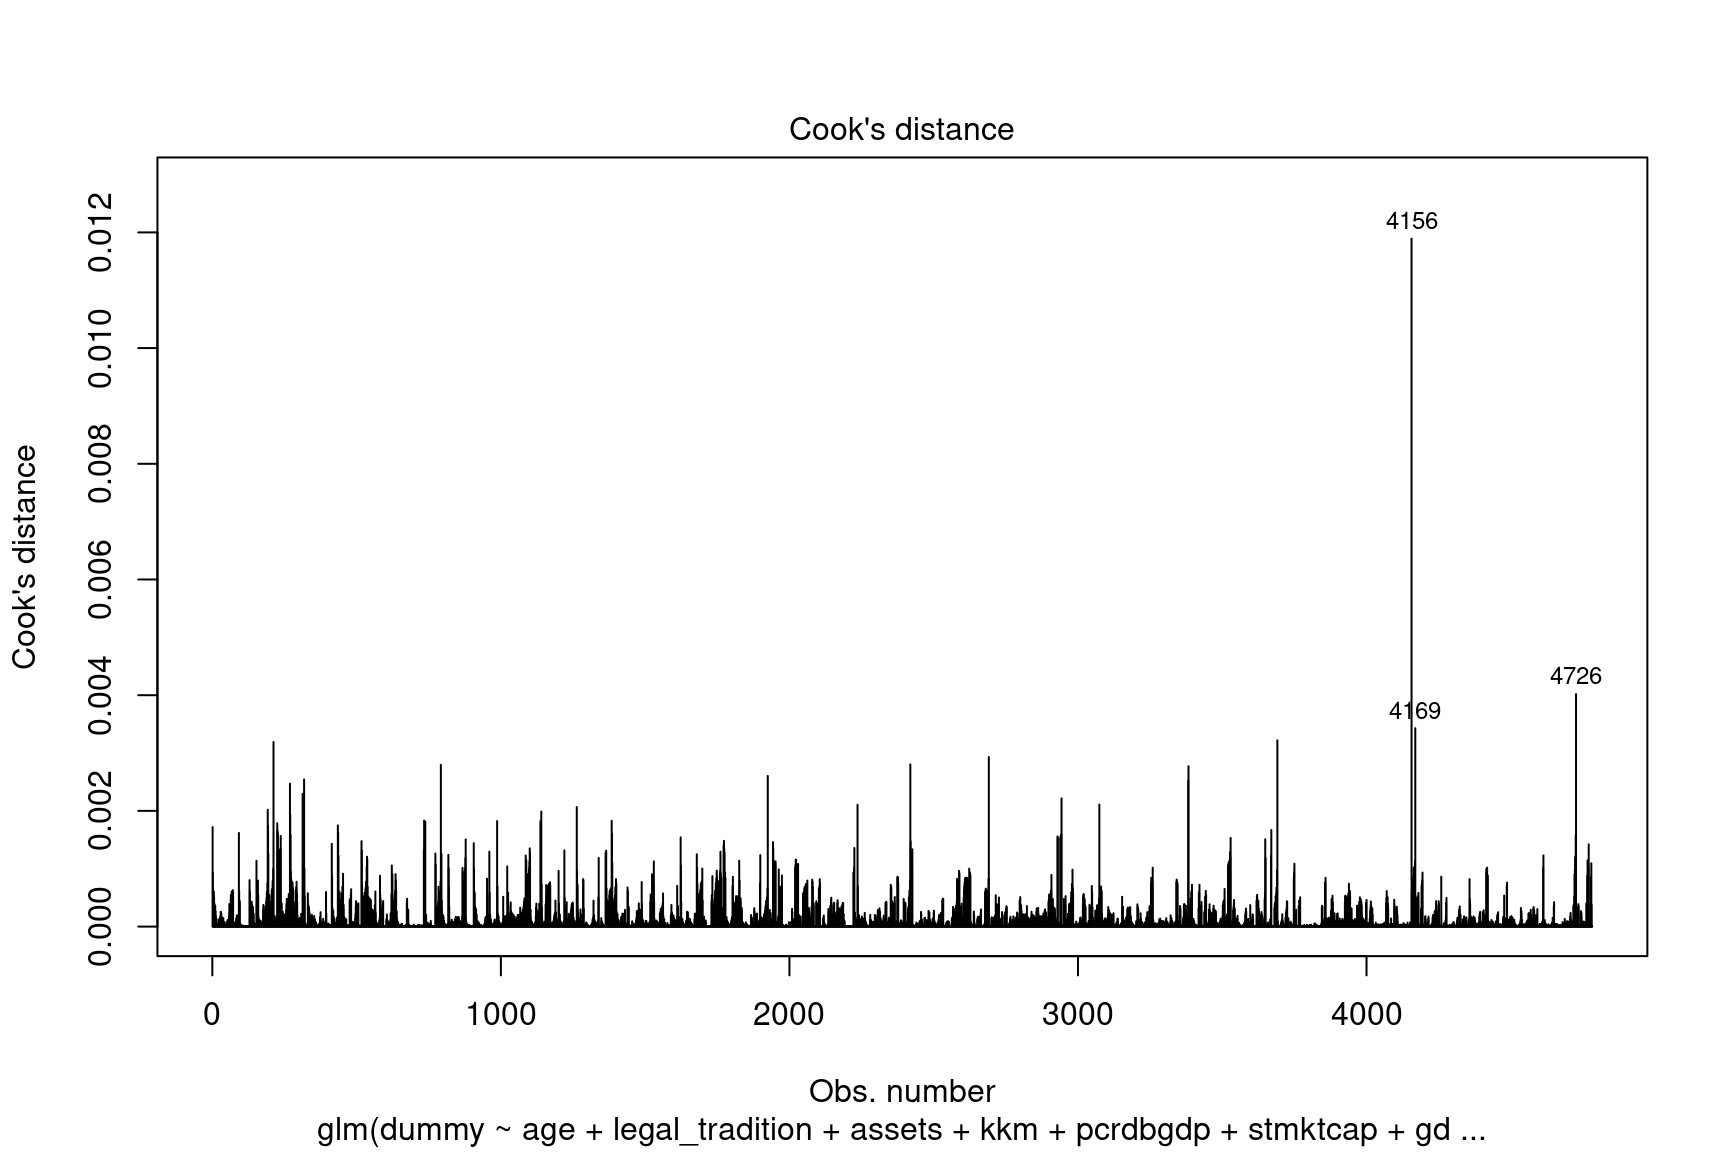
\includegraphics{04-tables_files/figure-latex/unnamed-chunk-40-1.pdf}
\caption{\label{fig:unnamed-chunk-40}Normal QQ Plots for Regressions Using Winsorized Data}
\end{figure}

\newpage

\begin{Shaded}
\begin{Highlighting}[]
\FunctionTok{second\_plotter}\NormalTok{(}\AttributeTok{data =}\NormalTok{ my\_data, }\AttributeTok{x =}\NormalTok{ currentlegalstatus, }
        \AttributeTok{z =}\NormalTok{ currentlegalstatus,}
        \AttributeTok{y =}\NormalTok{ debt\_to\_equity\_ratio, }
        \AttributeTok{xlabel =} \StringTok{"Current Legal Status"}\NormalTok{, }
        \AttributeTok{ylabel =} \StringTok{"Debt to Equity Ratio (Log Scale)"}\NormalTok{, }
        \AttributeTok{title =} \StringTok{""}\NormalTok{) }\SpecialCharTok{+}
  
\FunctionTok{second\_plotter}\NormalTok{(}\AttributeTok{data =}\NormalTok{ my\_data, }\AttributeTok{x =}\NormalTok{ currentlegalstatus, }
        \AttributeTok{z =}\NormalTok{ currentlegalstatus,}
        \AttributeTok{y =}\NormalTok{ deposits\_to\_total\_assets, }
        \AttributeTok{xlabel =} \StringTok{"Current Legal Status"}\NormalTok{, }
        \AttributeTok{ylabel =} \StringTok{"Donations to Assets Ratio (Log Scale)"}\NormalTok{, }
        \AttributeTok{title =} \StringTok{""}\NormalTok{)}
\end{Highlighting}
\end{Shaded}

\begin{verbatim}
## Warning: `guides(<scale> = FALSE)` is deprecated. Please use `guides(<scale> =
## "none")` instead.

## Warning: `guides(<scale> = FALSE)` is deprecated. Please use `guides(<scale> =
## "none")` instead.
\end{verbatim}

\begin{verbatim}
## Warning in self$trans$transform(x): NaNs produced
\end{verbatim}

\begin{verbatim}
## Warning: Transformation introduced infinite values in continuous y-axis
\end{verbatim}

\begin{verbatim}
## Warning in self$trans$transform(x): NaNs produced
\end{verbatim}

\begin{verbatim}
## Warning: Transformation introduced infinite values in continuous y-axis
\end{verbatim}

\begin{verbatim}
## Warning in self$trans$transform(x): NaNs produced
\end{verbatim}

\begin{verbatim}
## Warning: Transformation introduced infinite values in continuous y-axis
\end{verbatim}

\begin{verbatim}
## Warning: Removed 276 rows containing non-finite values (stat_ydensity).
\end{verbatim}

\begin{verbatim}
## Warning: Removed 276 rows containing non-finite values (stat_boxplot).
\end{verbatim}

\begin{verbatim}
## Warning: Removed 276 rows containing missing values (geom_point).
\end{verbatim}

\begin{verbatim}
## Warning: Transformation introduced infinite values in continuous y-axis

## Warning: Transformation introduced infinite values in continuous y-axis

## Warning: Transformation introduced infinite values in continuous y-axis
\end{verbatim}

\begin{verbatim}
## Warning: Removed 492 rows containing non-finite values (stat_ydensity).
\end{verbatim}

\begin{verbatim}
## Warning: Removed 492 rows containing non-finite values (stat_boxplot).
\end{verbatim}

\begin{verbatim}
## Warning: Removed 492 rows containing missing values (geom_point).
\end{verbatim}

\begin{figure}
\centering
\includegraphics{04-tables_files/figure-latex/unnamed-chunk-41-1.pdf}
\caption{\label{fig:unnamed-chunk-41}Debt to Equity Ratio by MFI Legal Status}
\end{figure}

\newpage

\begin{Shaded}
\begin{Highlighting}[]
\NormalTok{(my\_data }\SpecialCharTok{\%\textgreater{}\%} 
  
  \FunctionTok{group\_by}\NormalTok{(year) }\SpecialCharTok{\%\textgreater{}\%} 
  
  \FunctionTok{summarize}\NormalTok{(}\AttributeTok{mean\_de =} \FunctionTok{mean}\NormalTok{(debt\_to\_equity\_ratio, }\AttributeTok{na.rm =} \ConstantTok{TRUE}\NormalTok{), }
                               
  \AttributeTok{median\_de =} \FunctionTok{median}\NormalTok{(debt\_to\_equity\_ratio, }\AttributeTok{na.rm =} \ConstantTok{TRUE}\NormalTok{)) }\SpecialCharTok{\%\textgreater{}\%} 
  
  \FunctionTok{ggplot}\NormalTok{(}\AttributeTok{mapping =} \FunctionTok{aes}\NormalTok{(}\AttributeTok{x =}\NormalTok{ year, }\AttributeTok{y =}\NormalTok{ mean\_de), }\AttributeTok{color =} \StringTok{"skyblue"}\NormalTok{) }\SpecialCharTok{+} \FunctionTok{geom\_line}\NormalTok{() }\SpecialCharTok{+}
  
  \FunctionTok{geom\_line}\NormalTok{(}\AttributeTok{mapping =} \FunctionTok{aes}\NormalTok{(}\AttributeTok{x =}\NormalTok{ year, }\AttributeTok{y =}\NormalTok{ median\_de), }\AttributeTok{linetype =} \StringTok{"dashed"}\NormalTok{, }\AttributeTok{color =} \StringTok{"red"}\NormalTok{) }\SpecialCharTok{+}
  
  \FunctionTok{labs}\NormalTok{(}\AttributeTok{x =} \StringTok{"Year"}\NormalTok{, }\AttributeTok{y =} \StringTok{"Debt/Equity Ratio"}\NormalTok{, }\AttributeTok{title =} \StringTok{""}\NormalTok{, }
       \AttributeTok{caption =} \StringTok{"Authors, computation from MIX data"}\NormalTok{) }\SpecialCharTok{+} 
  
\NormalTok{  ggthemes}\SpecialCharTok{::}\FunctionTok{theme\_clean}\NormalTok{() }\SpecialCharTok{+}




\DocumentationTok{\#\# Percent of female borrowers {-} trends over time}
\NormalTok{my\_data }\SpecialCharTok{\%\textgreater{}\%} 
  
  \FunctionTok{group\_by}\NormalTok{(year, currentlegalstatus) }\SpecialCharTok{\%\textgreater{}\%} 
  
  \FunctionTok{summarize}\NormalTok{(}\AttributeTok{mean\_female =} \FunctionTok{mean}\NormalTok{(percent\_of\_female\_borrowers, }\AttributeTok{na.rm =} \ConstantTok{TRUE}\NormalTok{), }
                               
  \AttributeTok{median\_female =} \FunctionTok{median}\NormalTok{(percent\_of\_female\_borrowers, }\AttributeTok{na.rm =} \ConstantTok{TRUE}\NormalTok{)) }\SpecialCharTok{\%\textgreater{}\%} 
  
  \FunctionTok{ggplot}\NormalTok{(}\AttributeTok{mapping =} \FunctionTok{aes}\NormalTok{(}\AttributeTok{x =}\NormalTok{ year, }\AttributeTok{y =}\NormalTok{ mean\_female), }\AttributeTok{color =} \StringTok{"skyblue"}\NormalTok{) }\SpecialCharTok{+} \FunctionTok{geom\_line}\NormalTok{() }\SpecialCharTok{+}
  
  \FunctionTok{geom\_line}\NormalTok{(}\AttributeTok{mapping =} \FunctionTok{aes}\NormalTok{(}\AttributeTok{x =}\NormalTok{ year, }\AttributeTok{y =}\NormalTok{ median\_female), }\AttributeTok{linetype =} \StringTok{"dashed"}\NormalTok{, }\AttributeTok{color =} \StringTok{"red"}\NormalTok{) }\SpecialCharTok{+}
  
  \FunctionTok{labs}\NormalTok{(}\AttributeTok{x =} \StringTok{"Year"}\NormalTok{, }\AttributeTok{y =} \StringTok{"Percent of Female Borrowers"}\NormalTok{, }\AttributeTok{title =} \StringTok{""}\NormalTok{) }\SpecialCharTok{+} 
  
\NormalTok{  ggthemes}\SpecialCharTok{::}\FunctionTok{theme\_clean}\NormalTok{() }\SpecialCharTok{+} \FunctionTok{facet\_wrap}\NormalTok{(}\SpecialCharTok{\textasciitilde{}}\NormalTok{currentlegalstatus)) }\SpecialCharTok{/}



\DocumentationTok{\#\# Average loan Balance per borrower}
\NormalTok{(my\_data }\SpecialCharTok{\%\textgreater{}\%} 
  
  \FunctionTok{group\_by}\NormalTok{(year, currentlegalstatus) }\SpecialCharTok{\%\textgreater{}\%} 
  
  \FunctionTok{summarize}\NormalTok{(}\AttributeTok{mean\_average\_loan =} \FunctionTok{mean}\NormalTok{(average\_loan\_balance\_per\_borrower, }\AttributeTok{na.rm =} \ConstantTok{TRUE}\NormalTok{), }
                               
  \AttributeTok{median\_average\_loan =} \FunctionTok{median}\NormalTok{(average\_loan\_balance\_per\_borrower, }\AttributeTok{na.rm =} \ConstantTok{TRUE}\NormalTok{)) }\SpecialCharTok{\%\textgreater{}\%} 
  
  \FunctionTok{ggplot}\NormalTok{(}\AttributeTok{mapping =} \FunctionTok{aes}\NormalTok{(}\AttributeTok{x =}\NormalTok{ year, }\AttributeTok{y =}\NormalTok{ mean\_average\_loan), }\AttributeTok{color =} \StringTok{"skyblue"}\NormalTok{) }\SpecialCharTok{+} \FunctionTok{geom\_line}\NormalTok{() }\SpecialCharTok{+}
  
  \FunctionTok{geom\_line}\NormalTok{(}\AttributeTok{mapping =} \FunctionTok{aes}\NormalTok{(}\AttributeTok{x =}\NormalTok{ year, }\AttributeTok{y =}\NormalTok{ median\_average\_loan), }\AttributeTok{linetype =} \StringTok{"dashed"}\NormalTok{, }\AttributeTok{color =} \StringTok{"red"}\NormalTok{) }\SpecialCharTok{+}
  
  \FunctionTok{labs}\NormalTok{(}\AttributeTok{x =} \StringTok{"Year"}\NormalTok{, }\AttributeTok{y =} \StringTok{"Average Loan Balance"}\NormalTok{, }\AttributeTok{title =} \StringTok{"T"}\NormalTok{) }\SpecialCharTok{+} 
  
\NormalTok{  ggthemes}\SpecialCharTok{::}\FunctionTok{theme\_clean}\NormalTok{() }\SpecialCharTok{+} \FunctionTok{facet\_wrap}\NormalTok{(}\SpecialCharTok{\textasciitilde{}}\NormalTok{currentlegalstatus) }\SpecialCharTok{+}


\DocumentationTok{\#\# Gross loan portfolio to assets }
\NormalTok{my\_data }\SpecialCharTok{\%\textgreater{}\%} 
  
  \FunctionTok{group\_by}\NormalTok{(year, currentlegalstatus) }\SpecialCharTok{\%\textgreater{}\%} 
  
  \FunctionTok{summarize}\NormalTok{(}\AttributeTok{mean\_gross\_loans =} \FunctionTok{mean}\NormalTok{(gross\_loan\_portfolio\_to\_total\_assets, }\AttributeTok{na.rm =} \ConstantTok{TRUE}\NormalTok{), }
                               
  \AttributeTok{median\_gross\_loans =} \FunctionTok{median}\NormalTok{(gross\_loan\_portfolio\_to\_total\_assets, }\AttributeTok{na.rm =} \ConstantTok{TRUE}\NormalTok{)) }\SpecialCharTok{\%\textgreater{}\%} 
  
  \FunctionTok{ggplot}\NormalTok{(}\AttributeTok{mapping =} \FunctionTok{aes}\NormalTok{(}\AttributeTok{x =}\NormalTok{ year, }\AttributeTok{y =}\NormalTok{ mean\_gross\_loans), }\AttributeTok{color =} \StringTok{"skyblue"}\NormalTok{) }\SpecialCharTok{+} \FunctionTok{geom\_line}\NormalTok{() }\SpecialCharTok{+}
  
  \FunctionTok{geom\_line}\NormalTok{(}\AttributeTok{mapping =} \FunctionTok{aes}\NormalTok{(}\AttributeTok{x =}\NormalTok{ year, }\AttributeTok{y =}\NormalTok{ median\_gross\_loans), }\AttributeTok{linetype =} \StringTok{"dashed"}\NormalTok{, }\AttributeTok{color =} \StringTok{"red"}\NormalTok{) }\SpecialCharTok{+}
  
  \FunctionTok{labs}\NormalTok{(}\AttributeTok{x =} \StringTok{"Year"}\NormalTok{, }\AttributeTok{y =} \StringTok{"Gross Loans to Assets"}\NormalTok{, }\AttributeTok{title =} \StringTok{""}\NormalTok{) }\SpecialCharTok{+} 
  
\NormalTok{  ggthemes}\SpecialCharTok{::}\FunctionTok{theme\_clean}\NormalTok{() }\SpecialCharTok{+} \FunctionTok{facet\_wrap}\NormalTok{(}\SpecialCharTok{\textasciitilde{}}\NormalTok{currentlegalstatus))}
\end{Highlighting}
\end{Shaded}

\begin{verbatim}
## `summarise()` has grouped output by 'year'. You can override using the `.groups` argument.
## `summarise()` has grouped output by 'year'. You can override using the `.groups` argument.
## `summarise()` has grouped output by 'year'. You can override using the `.groups` argument.
\end{verbatim}

\begin{figure}
\centering
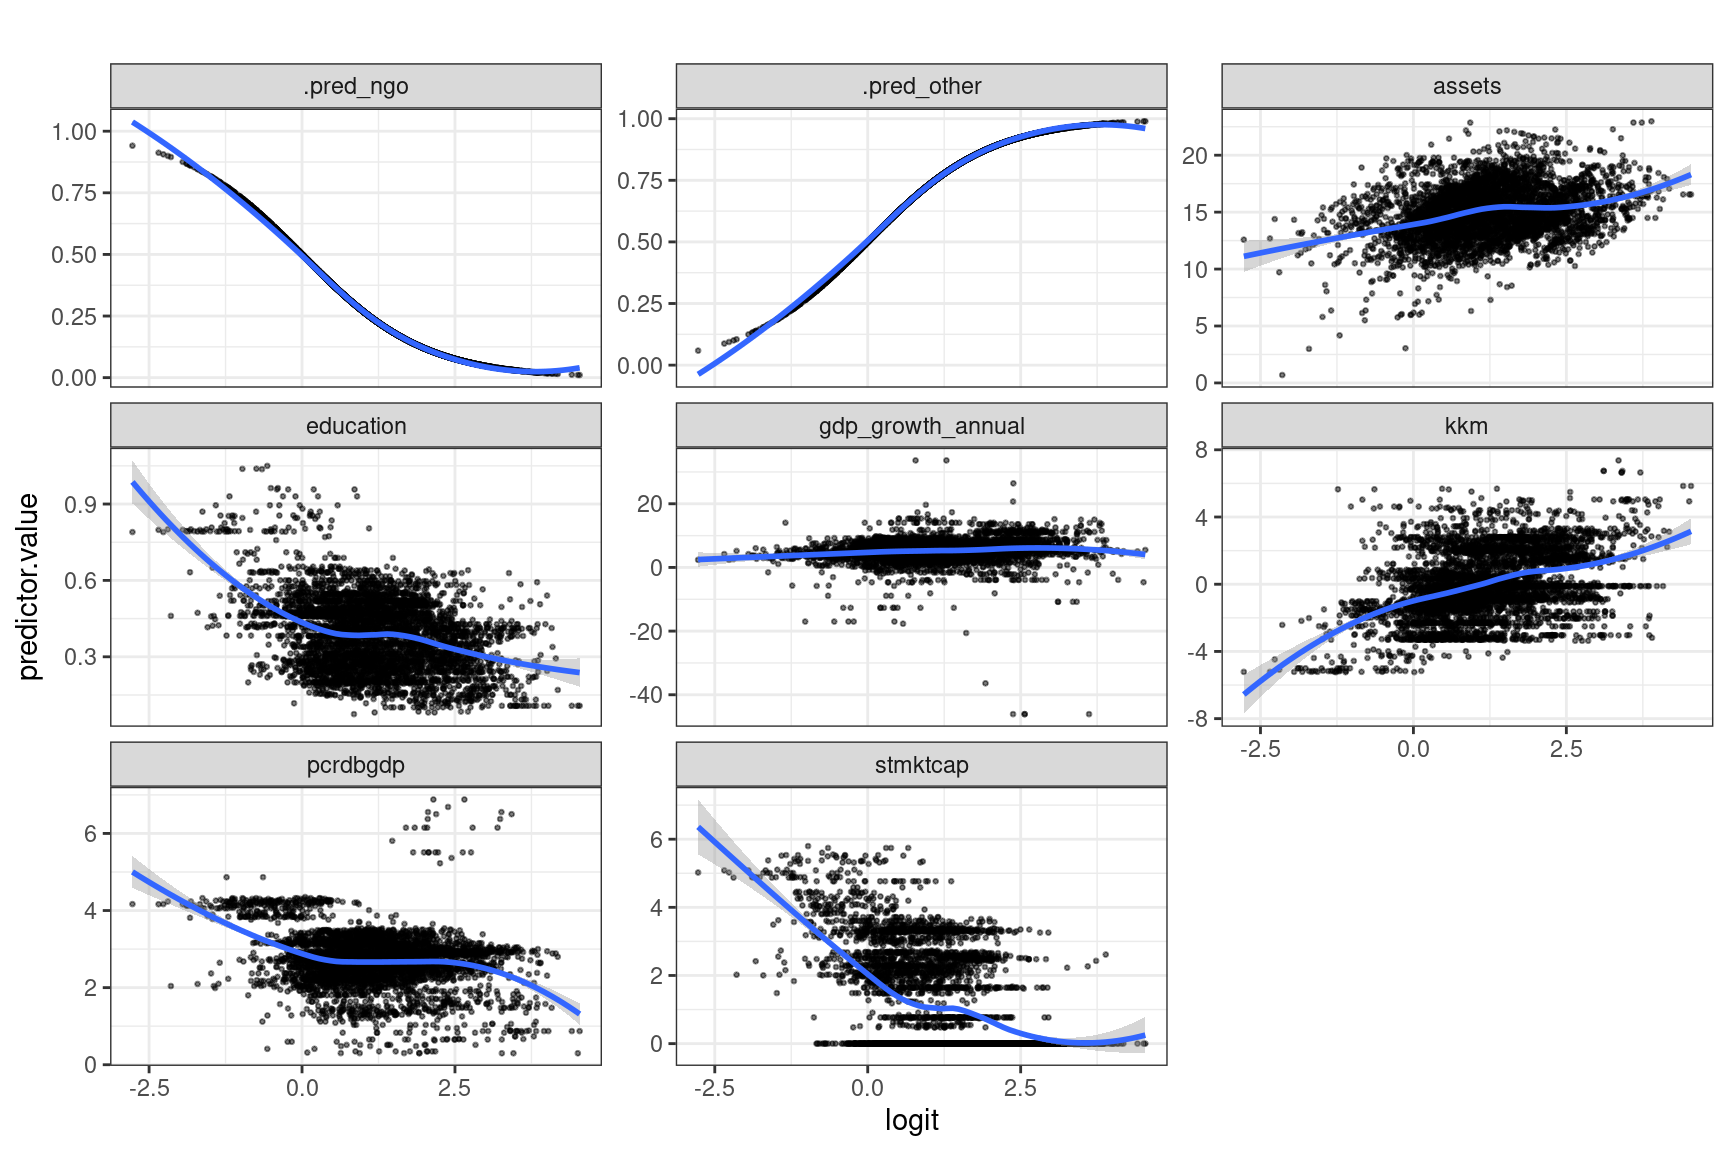
\includegraphics{04-tables_files/figure-latex/unnamed-chunk-42-1.pdf}
\caption{\label{fig:unnamed-chunk-42}Trends in the Percent of Female Borrowers by Legal Tradition}
\end{figure}

\end{landscape}


%%%%% REFERENCES

% JEM: Quote for the top of references (just like a chapter quote if you're using them).  Comment to skip.
% \begin{savequote}[8cm]
% The first kind of intellectual and artistic personality belongs to the hedgehogs, the second to the foxes \dots
%   \qauthor{--- Sir Isaiah Berlin \cite{berlin_hedgehog_2013}}
% \end{savequote}

\setlength{\baselineskip}{0pt} % JEM: Single-space References

{\renewcommand*\MakeUppercase[1]{#1}%
\printbibliography[heading=bibintoc,title={\bibtitle}]}

\end{document}
